% Options for packages loaded elsewhere
\PassOptionsToPackage{unicode}{hyperref}
\PassOptionsToPackage{hyphens}{url}
\PassOptionsToPackage{dvipsnames,svgnames,x11names}{xcolor}
%
\documentclass[
  letterpaper,
  DIV=11,
  numbers=noendperiod]{scrreprt}

\usepackage{amsmath,amssymb}
\usepackage{iftex}
\ifPDFTeX
  \usepackage[T1]{fontenc}
  \usepackage[utf8]{inputenc}
  \usepackage{textcomp} % provide euro and other symbols
\else % if luatex or xetex
  \usepackage{unicode-math}
  \defaultfontfeatures{Scale=MatchLowercase}
  \defaultfontfeatures[\rmfamily]{Ligatures=TeX,Scale=1}
\fi
\usepackage{lmodern}
\ifPDFTeX\else  
    % xetex/luatex font selection
\fi
% Use upquote if available, for straight quotes in verbatim environments
\IfFileExists{upquote.sty}{\usepackage{upquote}}{}
\IfFileExists{microtype.sty}{% use microtype if available
  \usepackage[]{microtype}
  \UseMicrotypeSet[protrusion]{basicmath} % disable protrusion for tt fonts
}{}
\makeatletter
\@ifundefined{KOMAClassName}{% if non-KOMA class
  \IfFileExists{parskip.sty}{%
    \usepackage{parskip}
  }{% else
    \setlength{\parindent}{0pt}
    \setlength{\parskip}{6pt plus 2pt minus 1pt}}
}{% if KOMA class
  \KOMAoptions{parskip=half}}
\makeatother
\usepackage{xcolor}
\setlength{\emergencystretch}{3em} % prevent overfull lines
\setcounter{secnumdepth}{5}
% Make \paragraph and \subparagraph free-standing
\makeatletter
\ifx\paragraph\undefined\else
  \let\oldparagraph\paragraph
  \renewcommand{\paragraph}{
    \@ifstar
      \xxxParagraphStar
      \xxxParagraphNoStar
  }
  \newcommand{\xxxParagraphStar}[1]{\oldparagraph*{#1}\mbox{}}
  \newcommand{\xxxParagraphNoStar}[1]{\oldparagraph{#1}\mbox{}}
\fi
\ifx\subparagraph\undefined\else
  \let\oldsubparagraph\subparagraph
  \renewcommand{\subparagraph}{
    \@ifstar
      \xxxSubParagraphStar
      \xxxSubParagraphNoStar
  }
  \newcommand{\xxxSubParagraphStar}[1]{\oldsubparagraph*{#1}\mbox{}}
  \newcommand{\xxxSubParagraphNoStar}[1]{\oldsubparagraph{#1}\mbox{}}
\fi
\makeatother

\usepackage{color}
\usepackage{fancyvrb}
\newcommand{\VerbBar}{|}
\newcommand{\VERB}{\Verb[commandchars=\\\{\}]}
\DefineVerbatimEnvironment{Highlighting}{Verbatim}{commandchars=\\\{\}}
% Add ',fontsize=\small' for more characters per line
\usepackage{framed}
\definecolor{shadecolor}{RGB}{241,243,245}
\newenvironment{Shaded}{\begin{snugshade}}{\end{snugshade}}
\newcommand{\AlertTok}[1]{\textcolor[rgb]{0.68,0.00,0.00}{#1}}
\newcommand{\AnnotationTok}[1]{\textcolor[rgb]{0.37,0.37,0.37}{#1}}
\newcommand{\AttributeTok}[1]{\textcolor[rgb]{0.40,0.45,0.13}{#1}}
\newcommand{\BaseNTok}[1]{\textcolor[rgb]{0.68,0.00,0.00}{#1}}
\newcommand{\BuiltInTok}[1]{\textcolor[rgb]{0.00,0.23,0.31}{#1}}
\newcommand{\CharTok}[1]{\textcolor[rgb]{0.13,0.47,0.30}{#1}}
\newcommand{\CommentTok}[1]{\textcolor[rgb]{0.37,0.37,0.37}{#1}}
\newcommand{\CommentVarTok}[1]{\textcolor[rgb]{0.37,0.37,0.37}{\textit{#1}}}
\newcommand{\ConstantTok}[1]{\textcolor[rgb]{0.56,0.35,0.01}{#1}}
\newcommand{\ControlFlowTok}[1]{\textcolor[rgb]{0.00,0.23,0.31}{\textbf{#1}}}
\newcommand{\DataTypeTok}[1]{\textcolor[rgb]{0.68,0.00,0.00}{#1}}
\newcommand{\DecValTok}[1]{\textcolor[rgb]{0.68,0.00,0.00}{#1}}
\newcommand{\DocumentationTok}[1]{\textcolor[rgb]{0.37,0.37,0.37}{\textit{#1}}}
\newcommand{\ErrorTok}[1]{\textcolor[rgb]{0.68,0.00,0.00}{#1}}
\newcommand{\ExtensionTok}[1]{\textcolor[rgb]{0.00,0.23,0.31}{#1}}
\newcommand{\FloatTok}[1]{\textcolor[rgb]{0.68,0.00,0.00}{#1}}
\newcommand{\FunctionTok}[1]{\textcolor[rgb]{0.28,0.35,0.67}{#1}}
\newcommand{\ImportTok}[1]{\textcolor[rgb]{0.00,0.46,0.62}{#1}}
\newcommand{\InformationTok}[1]{\textcolor[rgb]{0.37,0.37,0.37}{#1}}
\newcommand{\KeywordTok}[1]{\textcolor[rgb]{0.00,0.23,0.31}{\textbf{#1}}}
\newcommand{\NormalTok}[1]{\textcolor[rgb]{0.00,0.23,0.31}{#1}}
\newcommand{\OperatorTok}[1]{\textcolor[rgb]{0.37,0.37,0.37}{#1}}
\newcommand{\OtherTok}[1]{\textcolor[rgb]{0.00,0.23,0.31}{#1}}
\newcommand{\PreprocessorTok}[1]{\textcolor[rgb]{0.68,0.00,0.00}{#1}}
\newcommand{\RegionMarkerTok}[1]{\textcolor[rgb]{0.00,0.23,0.31}{#1}}
\newcommand{\SpecialCharTok}[1]{\textcolor[rgb]{0.37,0.37,0.37}{#1}}
\newcommand{\SpecialStringTok}[1]{\textcolor[rgb]{0.13,0.47,0.30}{#1}}
\newcommand{\StringTok}[1]{\textcolor[rgb]{0.13,0.47,0.30}{#1}}
\newcommand{\VariableTok}[1]{\textcolor[rgb]{0.07,0.07,0.07}{#1}}
\newcommand{\VerbatimStringTok}[1]{\textcolor[rgb]{0.13,0.47,0.30}{#1}}
\newcommand{\WarningTok}[1]{\textcolor[rgb]{0.37,0.37,0.37}{\textit{#1}}}

\providecommand{\tightlist}{%
  \setlength{\itemsep}{0pt}\setlength{\parskip}{0pt}}\usepackage{longtable,booktabs,array}
\usepackage{calc} % for calculating minipage widths
% Correct order of tables after \paragraph or \subparagraph
\usepackage{etoolbox}
\makeatletter
\patchcmd\longtable{\par}{\if@noskipsec\mbox{}\fi\par}{}{}
\makeatother
% Allow footnotes in longtable head/foot
\IfFileExists{footnotehyper.sty}{\usepackage{footnotehyper}}{\usepackage{footnote}}
\makesavenoteenv{longtable}
\usepackage{graphicx}
\makeatletter
\def\maxwidth{\ifdim\Gin@nat@width>\linewidth\linewidth\else\Gin@nat@width\fi}
\def\maxheight{\ifdim\Gin@nat@height>\textheight\textheight\else\Gin@nat@height\fi}
\makeatother
% Scale images if necessary, so that they will not overflow the page
% margins by default, and it is still possible to overwrite the defaults
% using explicit options in \includegraphics[width, height, ...]{}
\setkeys{Gin}{width=\maxwidth,height=\maxheight,keepaspectratio}
% Set default figure placement to htbp
\makeatletter
\def\fps@figure{htbp}
\makeatother
% definitions for citeproc citations
\NewDocumentCommand\citeproctext{}{}
\NewDocumentCommand\citeproc{mm}{%
  \begingroup\def\citeproctext{#2}\cite{#1}\endgroup}
\makeatletter
 % allow citations to break across lines
 \let\@cite@ofmt\@firstofone
 % avoid brackets around text for \cite:
 \def\@biblabel#1{}
 \def\@cite#1#2{{#1\if@tempswa , #2\fi}}
\makeatother
\newlength{\cslhangindent}
\setlength{\cslhangindent}{1.5em}
\newlength{\csllabelwidth}
\setlength{\csllabelwidth}{3em}
\newenvironment{CSLReferences}[2] % #1 hanging-indent, #2 entry-spacing
 {\begin{list}{}{%
  \setlength{\itemindent}{0pt}
  \setlength{\leftmargin}{0pt}
  \setlength{\parsep}{0pt}
  % turn on hanging indent if param 1 is 1
  \ifodd #1
   \setlength{\leftmargin}{\cslhangindent}
   \setlength{\itemindent}{-1\cslhangindent}
  \fi
  % set entry spacing
  \setlength{\itemsep}{#2\baselineskip}}}
 {\end{list}}
\usepackage{calc}
\newcommand{\CSLBlock}[1]{\hfill\break\parbox[t]{\linewidth}{\strut\ignorespaces#1\strut}}
\newcommand{\CSLLeftMargin}[1]{\parbox[t]{\csllabelwidth}{\strut#1\strut}}
\newcommand{\CSLRightInline}[1]{\parbox[t]{\linewidth - \csllabelwidth}{\strut#1\strut}}
\newcommand{\CSLIndent}[1]{\hspace{\cslhangindent}#1}

\KOMAoption{captions}{tableheading}
\makeatletter
\@ifpackageloaded{tcolorbox}{}{\usepackage[skins,breakable]{tcolorbox}}
\@ifpackageloaded{fontawesome5}{}{\usepackage{fontawesome5}}
\definecolor{quarto-callout-color}{HTML}{909090}
\definecolor{quarto-callout-note-color}{HTML}{0758E5}
\definecolor{quarto-callout-important-color}{HTML}{CC1914}
\definecolor{quarto-callout-warning-color}{HTML}{EB9113}
\definecolor{quarto-callout-tip-color}{HTML}{00A047}
\definecolor{quarto-callout-caution-color}{HTML}{FC5300}
\definecolor{quarto-callout-color-frame}{HTML}{acacac}
\definecolor{quarto-callout-note-color-frame}{HTML}{4582ec}
\definecolor{quarto-callout-important-color-frame}{HTML}{d9534f}
\definecolor{quarto-callout-warning-color-frame}{HTML}{f0ad4e}
\definecolor{quarto-callout-tip-color-frame}{HTML}{02b875}
\definecolor{quarto-callout-caution-color-frame}{HTML}{fd7e14}
\makeatother
\makeatletter
\@ifpackageloaded{bookmark}{}{\usepackage{bookmark}}
\makeatother
\makeatletter
\@ifpackageloaded{caption}{}{\usepackage{caption}}
\AtBeginDocument{%
\ifdefined\contentsname
  \renewcommand*\contentsname{Table of contents}
\else
  \newcommand\contentsname{Table of contents}
\fi
\ifdefined\listfigurename
  \renewcommand*\listfigurename{List of Figures}
\else
  \newcommand\listfigurename{List of Figures}
\fi
\ifdefined\listtablename
  \renewcommand*\listtablename{List of Tables}
\else
  \newcommand\listtablename{List of Tables}
\fi
\ifdefined\figurename
  \renewcommand*\figurename{Figure}
\else
  \newcommand\figurename{Figure}
\fi
\ifdefined\tablename
  \renewcommand*\tablename{Table}
\else
  \newcommand\tablename{Table}
\fi
}
\@ifpackageloaded{float}{}{\usepackage{float}}
\floatstyle{ruled}
\@ifundefined{c@chapter}{\newfloat{codelisting}{h}{lop}}{\newfloat{codelisting}{h}{lop}[chapter]}
\floatname{codelisting}{Listing}
\newcommand*\listoflistings{\listof{codelisting}{List of Listings}}
\usepackage{amsthm}
\theoremstyle{definition}
\newtheorem{exercise}{Exercise}[chapter]
\theoremstyle{remark}
\AtBeginDocument{\renewcommand*{\proofname}{Proof}}
\newtheorem*{remark}{Remark}
\newtheorem*{solution}{Solution}
\newtheorem{refremark}{Remark}[chapter]
\newtheorem{refsolution}{Solution}[chapter]
\makeatother
\makeatletter
\makeatother
\makeatletter
\@ifpackageloaded{caption}{}{\usepackage{caption}}
\@ifpackageloaded{subcaption}{}{\usepackage{subcaption}}
\makeatother
\newcounter{quartocallouttipno}
\newcommand{\quartocallouttip}[1]{\refstepcounter{quartocallouttipno}\label{#1}}

\ifLuaTeX
  \usepackage{selnolig}  % disable illegal ligatures
\fi
\usepackage{bookmark}

\IfFileExists{xurl.sty}{\usepackage{xurl}}{} % add URL line breaks if available
\urlstyle{same} % disable monospaced font for URLs
\hypersetup{
  pdftitle={Modeling Life},
  pdfauthor={Theoretical Biology Group, Utrecht University},
  colorlinks=true,
  linkcolor={blue},
  filecolor={Maroon},
  citecolor={Blue},
  urlcolor={Blue},
  pdfcreator={LaTeX via pandoc}}


\title{Modeling Life}
\author{Theoretical Biology Group, Utrecht University}
\date{2025-04-24}

\begin{document}
\maketitle

\renewcommand*\contentsname{Table of contents}
{
\hypersetup{linkcolor=}
\setcounter{tocdepth}{2}
\tableofcontents
}

\chapter*{Modeling life}\label{modeling}
\addcontentsline{toc}{chapter}{Modeling life}

\markboth{Modeling life}{Modeling life}

This website accompanies the Modeling Life course at Utrecht University.
It primarily serves as a central hub for all the practicals
(werkcolleges), with the necessarily files, links and other resources
for each day.

Each practical has its own page containing background explanations, code
snippets, and questions that are designed for you to learn about the
models. Most of these exercises build directly on the lectures, allowing
you to explore biological questions---such as how morphogen gradients
form, how spatial patterns emerge, or how cells evolve to ``stick
together''.

You can navigate the site using the sidebar or the left. The
\href{general.qmd}{General Course Info} section outlines the general
course info (exams, learning goals, etc.). You can also find the
\href{schedule.qmd}{Schedule} on this website. The individual practicals
sections provides detailed instructions for each day. In the second part
of the course you will get even more experience doing things yourself by
working on a mini-project.

We hope you'll use this website actively. There's lots to read,
simulate, modify, and explore.

\emph{Note: the Modeling Life course is new. This website is to help
you, but is by no means perfect. Please let us know if you see any
mistakes, typo's or other issues. Any constructive feedback on how to
make things better and easier for you is always welcome.}

\part{Course information}

\chapter{General course info}\label{general}

Our names, email addresses, an overview of the course content, learning
goals, tips, grading, group formation, usage of Brightspace, materials
they need, required attendencee, and feedback is welcome blabla.

\chapter{Schedule}\label{schedule}

\section*{WEEK 1}\label{week-1}
\addcontentsline{toc}{section}{WEEK 1}

\markright{WEEK 1}

Nov 10, 2025 -- Welcome and Intro to Python (\textbf{HC} 13:15-17:00).

Nov 11, 2025 -- Pattern formation I: Gradients and segments (\textbf{HC}
10:00-12:45 and \textbf{WC1} 13:15-17:00).

Nov 13, 2025 -- Pattern formation II: Turing Digit patterning
(\textbf{HC} 10:00-12:45 and \textbf{WC2} 13:15-17:00).

\section*{WEEK 2}\label{week-2}
\addcontentsline{toc}{section}{WEEK 2}

\markright{WEEK 2}

Nov 17, 2025 -- Guest lecture: Max Rietkerk, Ecosystem's spatial
patterns (\textbf{HC} 13:15-17:00).

Nov 18, 2025 -- Pattern formation III: Clock and Wavefront (\textbf{HC}
10:00-12:45 and \textbf{WC3} 13:15-17:00).

Nov 20, 2025 -- Morphogenesis: Cell sorting (\textbf{HC} 10:00-12:45 and
\textbf{WC4} 13:15-17:00).

\section*{WEEK 3}\label{week-3}
\addcontentsline{toc}{section}{WEEK 3}

\markright{WEEK 3}

Nov 24, 2025 -- Guest lecture: Ina Sonnen, Signal encoding in
multicellular systems (\textbf{HC} 13:15-17:00).

Nov 25, 2025 -- Cell differentiation: gene regulation in time
(\textbf{HC} 10:00-12:45 and \textbf{WC5} 13:15-17:00).

Nov 27, 2025 -- Cell differentiation: gene regulation in space
(\textbf{HC} 10:00-12:45 and \textbf{WC6} 13:15-17:00).

\section*{WEEK 4}\label{week-4}
\addcontentsline{toc}{section}{WEEK 4}

\markright{WEEK 4}

Dec 1, 2025 -- Guest lectures: Vivek Bhardwak and Kaisa Kajala, What is
a cell type? genomic and functional perspectives (\textbf{HC}
13:15-17:00).

Dec 2, 2025 -- Environment and Development (\textbf{HC} 10:00-12:45 and
\textbf{WC7} 13:15-17:00).

Dec 4, 2025 -- Evolving populations I: Sticky cells (\textbf{HC}
10:00-12:45 and \textbf{WC8} 13:15-17:00).

\section*{WEEK 5}\label{week-5}
\addcontentsline{toc}{section}{WEEK 5}

\markright{WEEK 5}

Dec 8, 2025 -- Guest lecture: Rutger Hermsen (\textbf{HC} 13:15-17:00).

Dec 9, 2025 - Evolving populations II: Genotype-phenotype map
(\textbf{HC} 10:00-12:45 and \textbf{WC9} 13:15-17:00).

Dec 11, 2025 - Evolving populations III: Microbial communities
(\textbf{HC} 10:00-12:45 and \textbf{WC10} 13:15-17:00).

\section*{WEEK 6 (self-study and
exam)}\label{week-6-self-study-and-exam}
\addcontentsline{toc}{section}{WEEK 6 (self-study and exam)}

\markright{WEEK 6 (self-study and exam)}

Dec 18, 2025 --Exam

\section*{WEEK 7-9 (mini projects)}\label{week-7-9-mini-projects}
\addcontentsline{toc}{section}{WEEK 7-9 (mini projects)}

\markright{WEEK 7-9 (mini projects)}

Jan 6, 2026 - Miniprojects presentation and making teams

Following weeks you will have classrooms to work on your miniprojects
(13:15-17:00). Also, you should schedule meetings with your supervisor
to discuss progress of your miniproject.

\section*{WEEK 10 (mini symposium)}\label{week-10-mini-symposium}
\addcontentsline{toc}{section}{WEEK 10 (mini symposium)}

\markright{WEEK 10 (mini symposium)}

Jan 29, 2026 - Miniprojects final presentation

\part{I) Pattern formation}

\chapter{Introduction}\label{introduction}

\subsection{TODO}\label{todo}

\begin{itemize}
\tightlist
\item
  Write a short intro on pattern formation part of the practicals.
\end{itemize}

\chapter{\texorpdfstring{Pattern formation I Gradients and
segments}{Pattern formation I   Gradients and segments}}\label{pattern-formation-i-gradients-and-segments}

\section{Morphogen Gradients and
Patterning}\label{morphogen-gradients-and-patterning}

In this practical, we a going to look at how an organism can form
segments along its body axis . The mathematical model that we will
implement and study is an implementation of the so-called French flag
conceptual model first proposed by Lewis Wolpert (Wolpert 1969). It
assumes the spatially graded expression of a morphogen ``M'' that
influences the expression of some downstream genes A, B and C. Their
expression is often visualized by red, white and blue and the arising
pattern resembles the French flag, hence the name (see the power of
visualization).

One of the most well-studied organisms when it comes to body axis
segmentation (although its segmentation mechanism is evolutionary
derived and a-typical!) is the development of the fruit fly Drosophila
melanogaster. Supporting the ideas of Wolpert, it was found that through
tethering maternal Bicoid mRNA to one side of the embryo, Bicoid protein
can form a gradient extending along the anterior-posterior axis, with so
called gap genes as a first tier in the segmentation hierarchy
differentially responding to different Bicoid protein levels (Driever
and Nüsslein-Volhard 1988). Later it was found that often at least two
opposing morphogen gradients drive downstream gene expression and genes
typically respond to multiple inputs.

\section{Mathematical modeling - integrating multiple
signals}\label{mathematical-modeling---integrating-multiple-signals}

Promotors/enhancers driving gene expression frequently make use of so
called OR and AND gates to integrate inputs from different transcription
factors. An OR gate can be implemented mathematically with a sum of the
effect of the transcription factors, while an AND can be implemented
mathematically with a product. Some examples:

\begin{itemize}
\tightlist
\item
  \(\frac{dX}{dt} = a(\text{tf1}) + b(\text{tf2})\): Gene X is induced
  by transcription factor 1 and 2 in an OR fashion, either
  \(a(\text{tf1})\) or \(b(\text{tf2})\) needs to be high to give high
  transcription of X.
\item
  \(\frac{dY}{dt} = a(\text{tf1})\cdot b(\text{tf2})\): Gene Y is
  induced by transcription factor 1 and 2 in an AND fashion, both
  \(a(\text{tf1})\) and \(b(\text{tf2})\), which are being multiplied,
  need to be high to give high transcription of X.
\end{itemize}

Note that the shape of \(a(\text{tf1})\) and \(b(\text{tf2})\)
(increasing or decreasing function of the transcription factor)
determines whether tf1 and tf2 are repressing or activating.

\section{Python code}\label{python-code}

\begin{tcolorbox}[enhanced jigsaw, left=2mm, opacitybacktitle=0.6, toptitle=1mm, colbacktitle=quarto-callout-note-color!10!white, toprule=.15mm, coltitle=black, colframe=quarto-callout-note-color-frame, opacityback=0, title=\textcolor{quarto-callout-note-color}{\faInfo}\hspace{0.5em}{Starting code for this practical}, breakable, bottomtitle=1mm, rightrule=.15mm, titlerule=0mm, arc=.35mm, leftrule=.75mm, bottomrule=.15mm, colback=white]

\begin{Shaded}
\begin{Highlighting}[]
\ImportTok{import}\NormalTok{ numpy }\ImportTok{as}\NormalTok{ np}
\ImportTok{import}\NormalTok{ matplotlib.pyplot }\ImportTok{as}\NormalTok{ plt}

\CommentTok{\# Parameters}
\NormalTok{Lx }\OperatorTok{=} \FloatTok{40.0}  \CommentTok{\# Length of the domain in x in microm}
\NormalTok{Ly }\OperatorTok{=} \FloatTok{10.0}  \CommentTok{\# Length of the domain in y in microm}
\NormalTok{T }\OperatorTok{=} \DecValTok{200}  \CommentTok{\# Total time in seconds}
\NormalTok{dx }\OperatorTok{=} \FloatTok{0.5}  \CommentTok{\# Grid spacing in x}
\NormalTok{dt }\OperatorTok{=} \FloatTok{0.1}  \CommentTok{\# Time step}
\NormalTok{nx }\OperatorTok{=} \BuiltInTok{int}\NormalTok{(Lx}\OperatorTok{/}\NormalTok{dx)}\OperatorTok{+}\DecValTok{2}  \CommentTok{\# Number of grid points in x + padding grid points}
\NormalTok{ny }\OperatorTok{=} \BuiltInTok{int}\NormalTok{(Ly}\OperatorTok{/}\NormalTok{dx)}\OperatorTok{+}\DecValTok{2}  \CommentTok{\# Number of grid points in y + padding grid points}
\CommentTok{\# Padding grid points to account for boundary conditions}
\NormalTok{nt }\OperatorTok{=} \BuiltInTok{int}\NormalTok{(T}\OperatorTok{/}\NormalTok{dt)  }\CommentTok{\# Number of time steps}
\NormalTok{D }\OperatorTok{=} \FloatTok{0.4}  \CommentTok{\# Diffusion coefficient in mm\^{}2/s}
\NormalTok{decayM }\OperatorTok{=}\FloatTok{0.01} \CommentTok{\# Decay rate in 1/s}


\CommentTok{\# Parameters for A, B, C}
\NormalTok{... }\CommentTok{\# }\AlertTok{TODO}\CommentTok{ create parameters for A, B, C as needed in Q5}

\CommentTok{\# Stability criterion}
\ControlFlowTok{if}\NormalTok{ D }\OperatorTok{*}\NormalTok{ dt }\OperatorTok{/}\NormalTok{ dx}\OperatorTok{**}\DecValTok{2} \OperatorTok{\textgreater{}} \FloatTok{0.5}\NormalTok{:}
    \ControlFlowTok{raise} \PreprocessorTok{ValueError}\NormalTok{(}\StringTok{"Stability criterion not met"}\NormalTok{)}

\CommentTok{\# A, B and C are required for later exercises.}
\NormalTok{A }\OperatorTok{=}\NormalTok{ np.zeros((nx, ny))}
\NormalTok{B }\OperatorTok{=}\NormalTok{ np.zeros((nx, ny))}
\NormalTok{C }\OperatorTok{=}\NormalTok{ np.zeros((nx, ny))}

\CommentTok{\# Initial condition}
\NormalTok{u }\OperatorTok{=}\NormalTok{ np.zeros((nx, ny))}
\NormalTok{u[}\DecValTok{0}\NormalTok{, :] }\OperatorTok{=} \DecValTok{100}

\CommentTok{\# Reaction{-}diffusion equation}
\KeywordTok{def}\NormalTok{ reaction\_diffusion\_step(u, D, dt, dx, decay):}
\NormalTok{    un }\OperatorTok{=}\NormalTok{ u.copy()}
\NormalTok{    u[}\DecValTok{1}\NormalTok{:}\OperatorTok{{-}}\DecValTok{1}\NormalTok{, }\DecValTok{1}\NormalTok{:}\OperatorTok{{-}}\DecValTok{1}\NormalTok{] }\OperatorTok{=}\NormalTok{ un[}\DecValTok{1}\NormalTok{:}\OperatorTok{{-}}\DecValTok{1}\NormalTok{, }\DecValTok{1}\NormalTok{:}\OperatorTok{{-}}\DecValTok{1}\NormalTok{] }\OperatorTok{+}\NormalTok{  D }\OperatorTok{*}\NormalTok{dt }\OperatorTok{/}\NormalTok{ dx}\OperatorTok{**}\DecValTok{2} \OperatorTok{*}\NormalTok{ (un[}\DecValTok{2}\NormalTok{:, }\DecValTok{1}\NormalTok{:}\OperatorTok{{-}}\DecValTok{1}\NormalTok{] }\OperatorTok{+}\NormalTok{ un[:}\OperatorTok{{-}}\DecValTok{2}\NormalTok{, }\DecValTok{1}\NormalTok{:}\OperatorTok{{-}}\DecValTok{1}\NormalTok{] }\OperatorTok{+} \OperatorTok{\textbackslash{}}
\NormalTok{                    un[}\DecValTok{1}\NormalTok{:}\OperatorTok{{-}}\DecValTok{1}\NormalTok{, }\DecValTok{2}\NormalTok{:]  }\OperatorTok{+}\NormalTok{ un[}\DecValTok{1}\NormalTok{:}\OperatorTok{{-}}\DecValTok{1}\NormalTok{, :}\OperatorTok{{-}}\DecValTok{2}\NormalTok{] }\OperatorTok{{-}} \DecValTok{4} \OperatorTok{*}\NormalTok{ un[}\DecValTok{1}\NormalTok{:}\OperatorTok{{-}}\DecValTok{1}\NormalTok{, }\DecValTok{1}\NormalTok{:}\OperatorTok{{-}}\DecValTok{1}\NormalTok{]) }\OperatorTok{{-}} \OperatorTok{\textbackslash{}}
\NormalTok{                    decay }\OperatorTok{*}\NormalTok{ un[}\DecValTok{1}\NormalTok{:}\OperatorTok{{-}}\DecValTok{1}\NormalTok{, }\DecValTok{1}\NormalTok{:}\OperatorTok{{-}}\DecValTok{1}\NormalTok{] }\OperatorTok{*}\NormalTok{ dt}
    \CommentTok{\#\# for loop version to understand the equation}
    \CommentTok{\# for i in range(1, nx{-}1):}
    \CommentTok{\#     for j in range(1, ny{-}1):}
    \CommentTok{\#         u[i, j] = (un[i, j] +}
    \CommentTok{\#                    D * dt / dx**2 * (un[i+1, j] + un[i{-}1, j] {-} 2 * un[i, j] +}
    \CommentTok{\#                    un[i, j+1] + un[i, j{-}1] {-} 4 * un[i, j]) {-} decay * un[i, j] * dt)}
    \CommentTok{\#boundary conditions}
\NormalTok{    u[}\OperatorTok{{-}}\DecValTok{1}\NormalTok{, :] }\OperatorTok{=}\NormalTok{ (u[}\OperatorTok{{-}}\DecValTok{2}\NormalTok{, :]}\OperatorTok{/}\NormalTok{u[}\OperatorTok{{-}}\DecValTok{3}\NormalTok{, :])}\OperatorTok{*}\NormalTok{u[}\OperatorTok{{-}}\DecValTok{2}\NormalTok{, :]  }\ControlFlowTok{if} \BuiltInTok{sum}\NormalTok{(u[}\OperatorTok{{-}}\DecValTok{3}\NormalTok{, :]) }\OperatorTok{!=} \DecValTok{0} \ControlFlowTok{else}\NormalTok{ np.zeros(ny)}
    \CommentTok{\#to understand this line:}
    \CommentTok{\#if sum(u[{-}3, :]) != 0:}
    \CommentTok{\#    u[{-}1, :] = (u[{-}2, :]/u[{-}3, :])*u[{-}2, :]\#extrapolate from third to last row}
    \CommentTok{\#else:}
    \CommentTok{\#    u[{-}1, :] = np.zeros(ny) \#if already zero in third to last row, also zero in last row}
\NormalTok{    u[:, }\DecValTok{0}\NormalTok{] }\OperatorTok{=}\NormalTok{ u[:, }\DecValTok{1}\NormalTok{]}
\NormalTok{    u[:, }\OperatorTok{{-}}\DecValTok{1}\NormalTok{] }\OperatorTok{=}\NormalTok{ u[:, }\OperatorTok{{-}}\DecValTok{2}\NormalTok{]}

    \ControlFlowTok{return}\NormalTok{ u}

\KeywordTok{def}\NormalTok{ reaction\_diffusion\_gradient(t, u, D, dx, decay, switch\_time }\OperatorTok{=} \VariableTok{None}\NormalTok{, noise }\OperatorTok{=} \VariableTok{False}\NormalTok{):}
    \CommentTok{\textquotesingle{}\textquotesingle{}\textquotesingle{}}
\CommentTok{    Function to create a gradient in the u array that could decay after a certain time.}
\CommentTok{    t: current time step}
\CommentTok{    u: array to create the gradient in}
\CommentTok{    D: diffusion coefficient}
\CommentTok{    dx: grid spacing}
\CommentTok{    decay: decay rate}
\CommentTok{    switch\_time: time step after which the gradient decays. If no switch is desired, set to None}
\CommentTok{    noise: whether to add noise to the gradient}
\CommentTok{    \textquotesingle{}\textquotesingle{}\textquotesingle{}}
    \CommentTok{\# }\AlertTok{TODO}\CommentTok{ for student: write code for the noise and the switch.}
\NormalTok{    added\_noise }\OperatorTok{=}\NormalTok{ np.zeros\_like(u)  }\CommentTok{\# Initialize noise array}
    \ControlFlowTok{if}\NormalTok{ noise:}
\NormalTok{        ...  }\CommentTok{\# }\AlertTok{TODO}\CommentTok{: add noise generation code here for Q10}
    
    \ControlFlowTok{if}\NormalTok{ switch\_time }\KeywordTok{is} \VariableTok{None} \KeywordTok{or}\NormalTok{ t }\OperatorTok{\textless{}=}\NormalTok{ switch\_time:}
        \CommentTok{\# define a exponential decay gradient over the array in the x direction with numpy array operations using the index}
        \ControlFlowTok{for}\NormalTok{ i }\KeywordTok{in} \BuiltInTok{range}\NormalTok{(u.shape[}\DecValTok{0}\NormalTok{]):}
\NormalTok{            u[i, :] }\OperatorTok{=}\NormalTok{ np.maximum(}\DecValTok{100} \OperatorTok{*}\NormalTok{ np.exp(}\OperatorTok{{-}}\NormalTok{i}\OperatorTok{*}\NormalTok{dx}\OperatorTok{/}\NormalTok{np.sqrt(D}\OperatorTok{/}\NormalTok{decay))}\OperatorTok{+}\NormalTok{added\_noise[i, :], }\DecValTok{0}\NormalTok{)}
        \ControlFlowTok{return}\NormalTok{ u}
    \ControlFlowTok{if}\NormalTok{ t }\OperatorTok{\textgreater{}}\NormalTok{ switch\_time:}
\NormalTok{        ...}\CommentTok{\# }\AlertTok{TODO}\CommentTok{ Q7: implement a gradient that decays over time, otherwise return the original u array}
        \ControlFlowTok{return}\NormalTok{ u}
    \CommentTok{\# In all other cases, return the original u array        }
    \ControlFlowTok{return}\NormalTok{ u}

\KeywordTok{def}\NormalTok{ hill(x, Km, }\BuiltInTok{pow}\NormalTok{):}
    \CommentTok{"""Hill function for the reaction kinetics."""}
    \ControlFlowTok{return}\NormalTok{ (x}\OperatorTok{**}\BuiltInTok{pow}\NormalTok{) }\OperatorTok{/}\NormalTok{ (Km}\OperatorTok{**}\BuiltInTok{pow} \OperatorTok{+}\NormalTok{ x}\OperatorTok{**}\BuiltInTok{pow}\NormalTok{) }

\KeywordTok{def}\NormalTok{ ihill(y, Km, }\BuiltInTok{pow}\NormalTok{):}
    \CommentTok{"""Inverse Hill function for the reaction kinetics."""}
    \ControlFlowTok{return}\NormalTok{( (Km}\OperatorTok{**}\BuiltInTok{pow}\NormalTok{) }\OperatorTok{/}\NormalTok{ (y }\OperatorTok{**}\BuiltInTok{pow}  \OperatorTok{+}\NormalTok{ Km}\OperatorTok{**}\BuiltInTok{pow}\NormalTok{))}

\CommentTok{\# }\AlertTok{TODO}\CommentTok{ for student: write update functions for A, B, C as needed in Q5}


\CommentTok{\# initilize figure and axes for plotting}
\CommentTok{\# }\AlertTok{TODO}\CommentTok{ for student: Add a new axis for the ABC flag visualization as suggested in Q5}
\NormalTok{fig, (ax\_M, ax\_lines) }\OperatorTok{=}\NormalTok{ plt.subplots(}\DecValTok{2}\NormalTok{, figsize}\OperatorTok{=}\NormalTok{(}\DecValTok{10}\NormalTok{, }\DecValTok{8}\NormalTok{), gridspec\_kw}\OperatorTok{=}\NormalTok{\{}\StringTok{\textquotesingle{}height\_ratios\textquotesingle{}}\NormalTok{: [}\DecValTok{3}\NormalTok{, }\DecValTok{1}\NormalTok{]\})  }\CommentTok{\# Make the first graph 3 times the height of the second}

\CommentTok{\# Time{-}stepping simulation loop}
\ControlFlowTok{for}\NormalTok{ n }\KeywordTok{in} \BuiltInTok{range}\NormalTok{(nt):}
    \CommentTok{\# Update all variables}
\NormalTok{    u }\OperatorTok{=}\NormalTok{ reaction\_diffusion\_step(u, D, dt, dx, decayM)}
    \CommentTok{\# }\AlertTok{TODO}\CommentTok{ for student: use precomputed gradient, update A, B, C as needed in Q5}
    
    \ControlFlowTok{if}\NormalTok{ n }\OperatorTok{==} \DecValTok{0}\NormalTok{:  }\CommentTok{\# Initial plot}
\NormalTok{        imshow\_M\_plot }\OperatorTok{=}\NormalTok{ ax\_M.imshow(u.T, cmap}\OperatorTok{=}\StringTok{\textquotesingle{}viridis\textquotesingle{}}\NormalTok{, origin}\OperatorTok{=}\StringTok{\textquotesingle{}lower\textquotesingle{}}\NormalTok{, aspect}\OperatorTok{=}\StringTok{\textquotesingle{}auto\textquotesingle{}}\NormalTok{)}
\NormalTok{        ax\_M.set\_title(}\SpecialStringTok{f"Time: }\SpecialCharTok{\{}\NormalTok{n}\OperatorTok{*}\NormalTok{dt}\SpecialCharTok{\}}\SpecialStringTok{"}\NormalTok{)}
\NormalTok{        ax\_M.set\_xlabel(}\StringTok{\textquotesingle{}x direction\textquotesingle{}}\NormalTok{)}
\NormalTok{        ax\_M.set\_ylabel(}\StringTok{\textquotesingle{}y direction\textquotesingle{}}\NormalTok{)}
\NormalTok{        ax\_M.set\_xticks([])}
\NormalTok{        ax\_M.set\_yticks([])}

        \CommentTok{\# Plot the concentration at a specific y index (e.g., y=2)    }
\NormalTok{        line\_plot }\OperatorTok{=}\NormalTok{ ax\_lines.plot([x}\OperatorTok{*}\NormalTok{dx }\ControlFlowTok{for}\NormalTok{ x }\KeywordTok{in} \BuiltInTok{range}\NormalTok{(nx)], u[:, }\DecValTok{2}\NormalTok{], label}\OperatorTok{=}\StringTok{\textquotesingle{}M\textquotesingle{}}\NormalTok{, color}\OperatorTok{=}\StringTok{\textquotesingle{}green\textquotesingle{}}\NormalTok{)}
        \CommentTok{\# }\AlertTok{TODO}\CommentTok{: Add lines for A, B, C as needed in Q5}

        
\NormalTok{        ax\_lines.legend(loc}\OperatorTok{=}\StringTok{\textquotesingle{}upper right\textquotesingle{}}\NormalTok{)}
\NormalTok{        ax\_lines.set\_ylim(}\DecValTok{0}\NormalTok{, }\DecValTok{100}\NormalTok{)}
\NormalTok{        ax\_lines.tick\_params(axis}\OperatorTok{=}\StringTok{\textquotesingle{}y\textquotesingle{}}\NormalTok{)}
\NormalTok{        ax\_lines.set\_xlim(}\DecValTok{0}\NormalTok{, dx}\OperatorTok{*}\NormalTok{nx)}
\NormalTok{        ax\_lines.set\_xlabel(}\StringTok{\textquotesingle{}x\textquotesingle{}}\NormalTok{)}
\NormalTok{        ax\_lines.set\_ylabel(}\StringTok{\textquotesingle{}Concentration at y=2\textquotesingle{}}\NormalTok{)}
\NormalTok{        ax\_lines.tick\_params(axis}\OperatorTok{=}\StringTok{\textquotesingle{}x\textquotesingle{}}\NormalTok{)}

    \ControlFlowTok{if}\NormalTok{ n }\OperatorTok{\%} \DecValTok{20} \OperatorTok{==} \DecValTok{0}\NormalTok{:  }\CommentTok{\# Update plot every so many time steps}
        \CommentTok{\#update the imshow M plot with the new data}
\NormalTok{        imshow\_M\_plot.set\_data(u.T)}
\NormalTok{        ax\_M.set\_title(}\SpecialStringTok{f"Time: }\SpecialCharTok{\{}\NormalTok{n}\OperatorTok{*}\NormalTok{dt}\SpecialCharTok{\}}\SpecialStringTok{"}\NormalTok{)}
            
        \CommentTok{\# Update the line plots with new data}
\NormalTok{        line\_plot[}\DecValTok{0}\NormalTok{].set\_ydata(u[:, }\DecValTok{2}\NormalTok{])}
        \CommentTok{\# }\AlertTok{TODO}\CommentTok{: Update A, B, C line plots as needed in Q5}

\NormalTok{    plt.pause(}\FloatTok{0.001}\NormalTok{)  }\CommentTok{\# Pause to refresh the plot}

\CommentTok{\# And keep the last plot open}
\CommentTok{\# plt.show()}

\CommentTok{\# Or close the plot window when done}
\NormalTok{plt.close(fig)}
\end{Highlighting}
\end{Shaded}

\end{tcolorbox}

\section{Questions}\label{questions}

\begin{exercise}[Algorithmic
thinking]\protect\hypertarget{exr-test}{}\label{exr-test}

Have a look at the reaction-diffusion equation for the morphogen and the
implementation of it in the file
\texttt{morphogengradient\_to\_segments.py} in the
reaction\_diffusion\_step function, as well as at the initialization of
the array u. How is this different from the gradient formation modeling
we discussed during the lecture? What is done at the terminal boundary
in the length direction and why does this make sense? (hint:
outcommented we provided code doing essentially the same but not using
numpy arrays and hence written in a less compact matter to help you
understand what is happening)

\end{exercise}

\begin{exercise}[Important
concept]\protect\hypertarget{exr-plain}{}\label{exr-plain}

Play with the morphogen diffusion rate and the morphogen decay rate and
describe what happens. What happens in terms of dynamics and steady
state if you change both, but the ratio stays the same? Hint: it might
help to draw a horizontal line at a certain height to ease comparison.

\end{exercise}

\begin{exercise}[Biology \& mathematical
thinking]\protect\hypertarget{exr-plain}{}\label{exr-plain}

Next, we are going to introduce the genes A, B and C in the model. We
want these genes to be expressed dependent on M, and in the head, trunk
and tail respectively, so A on the left, B in the middle and C on the
right. Think of what conditions in terms of M should lead to expression
of A/B/C. What Hill functions (normal/inverse/any combination)
corresponds to those conditions? Write down (pen and paper, not in code)
full equations for the genes, do we need any other terms than just Hill
functions, would we need specific parameter conditions?

\end{exercise}

\begin{exercise}[Biology \& algorithmic/mathematical
thinking]\protect\hypertarget{exr-plain}{}\label{exr-plain}

From hereon we assume that the morphogen gradient reaches steady state
very quickly, and no longer use the numerical implementation of the
diffusion equation and instead work with a superimposed morphogen
profile defined by \texttt{reaction\_diffusion\_gradient} to save time.
(Hint: to not call the function any more use \# in front of where it is
called) Change the simulation loop such that it computes the morphogen
gradient once. What type of function is the superimposed morphogen
profile and how does this relate to question 2.

\end{exercise}

\begin{exercise}[Biology \& algorithmic/mathematical
thinking]\protect\hypertarget{exr-plain}{}\label{exr-plain}

~

\begin{enumerate}
\def\labelenumi{\alph{enumi}.}
\tightlist
\item
  Now create functions to update A, B and C according to your equations
  from the previous question. You may use the predefined hill and ihill
  functions that are provided in the code. For simplicity, you may keep
  most of the parameters the same across genes, but some have to be
  different to ensure the right location of the genes (see your
  reasoning to the previous question). (Hint: using array properties to
  update A/B/C, like in the reaction\_diffusion\_step function, makes
  your code run a lot faster than using for-loops)
\item
  Also make sure that the levels of A, B and C are updated in the
  simulation loop. (Hint: using array properties to update A/B/C, like
  in the reaction\_diffusion\_step function, makes your code run a lot
  faster than using for-loops)
\item
  Next, ensure A, B and C are visualized in the bottom plot axis (copy
  and adapt the code for the visualization of M). You can add an extra
  third axis to the plot to visualize the (French) flag pattern, by
  getting which of the three genes is maximal at each location with
  np.argmax(np.array({[}A, B, C{]}), axis=0)and turning that into an
  array of RGB colors of choice.
\item
  Do you get the expected ``French flag'' pattern? If not, think of why
  not and improve your equations from previous question, parameters or
  your code.
\end{enumerate}

\end{exercise}

\begin{exercise}[Biology]\protect\hypertarget{exr-plain}{}\label{exr-plain}

At some point in development, the morphogen gradient will disappear, for
example in the case of the Drosophila Bicoid gradient because the
maternal mRNA is degraded. Predict what will happen to the expression of
A,B and C (and hence the French flag pattern) if the morphogen gradient
disappears over time and assume A, B, and C are regulated by our
equations (first try think about this without actually simulating this).

\end{exercise}

\begin{exercise}[Algorithmic/mathematical
thinking]\protect\hypertarget{exr-plain}{}\label{exr-plain}

Now write the code in reaction\_diffusion\_gradient that updates the
morphogen concentration, such that after the time point A, B and C have
gotten close to equilibrium, the morphogen gradient gradually
disappears. Adapt the simulation loop where necessary and run your code:
was your prediction on A/B/C from the previous question correct? Why/why
not? Hint: you might need to increase the duration of your simulation,
especially if it takes a long time for A, B and C to reach equilibrium
(or you can change the parameters to speed things up by using same
production/degradation rate ratio yet higher absolute values of the
individual parameters).

\end{exercise}

\begin{exercise}[Biological \& mathematical
thinking]\protect\hypertarget{exr-plain}{}\label{exr-plain}

A, B and C cannot remain in a stable pattern if they are only influenced
by M. How can we stabilize the pattern in absence of M? Test your ideas
by creating new update functions for A, B and C and let these new
`rules' kick in at the same time when M starts to decline. Again, you
may find Hill functions useful and perhaps also the before/after switch
time structure used in reaction\_diffusion\_gradient for M. (Hint: think
about how the genes should affect each other, and assume that in this
new phase, when genes have already been initialized in absence of
repression the genes will be expressed). Can you maintain the expression
domains of A, B and C and does their shape change?

\end{exercise}

\begin{exercise}[Biology \& algorithmic/mathematical
thinking]\protect\hypertarget{exr-plain}{}\label{exr-plain}

A sudden switch from phase 1 (stable M gradient) to phase 2 (decaying M
gradient) resulting in the genes following different differential
equations is biologically implausible. In reality, genes have complex
promotors and enhancers integrating different inputs that arise in
different developmental stages. Try to come up with one integrated
expression for each gene, incorporating simultaneous input from the
morphogen gradient and the other genes. Create new update functions for
A/B/C and test your ideas. Can you get a stable pattern before and after
the decline in M? A couple of things you could consider: a. Think of how
positively and negatively M regulated expression behave once the
gradient starts declining: what is the best way to combine (AND/OR) that
with the regulation by the genes? a. Consider splitting up the M
regulated expression of middle gene B into a positive and negatively
regulated morphogen part before integrating the other genes inputs. a.
It is also possible to give certain genes a bit of a constant boost to
prevent their takeover by other genes due to timing issues

\end{exercise}

\begin{exercise}[Biology \& algorithmic/mathematical
thinking]\protect\hypertarget{exr-plain}{}\label{exr-plain}

Write code to get noise in the morphogen gradient, both in its steady
state and decaying phase. During which phase do the expression domains
of A, B and C suffer more from the noise. Explain why? How could we make
the system more robust in a manner that is also likely occurring in
nature?

\end{exercise}

\section{\texorpdfstring{\textsc{\textbf{Extra
questions}}}{Extra questions}}\label{extra-questions}

If you're done early or a master student, you can make these extra
questions. These questions need not be made in the order they are
provided, you can choose what you would like to investigate.

\begin{exercise}[Biological
thinking]\protect\hypertarget{exr-plain}{}\label{exr-plain}

Play with the size of the domain to see what happens to the gene
expression domains. What would this mean for an organism?

\end{exercise}

\begin{exercise}[Biological \& algorithmic
thinking]\protect\hypertarget{exr-plain}{}\label{exr-plain}

Various mechanisms have been proposed to ensure that the domains of the
morphogen controlled genes scale with the size of the domain. One
proposed mechanism suggests the existence of an also diffusible
``expander'' molecule which expression is repressed by the morphogen but
which itself either represses the degradation of the morphogen or
enhances its diffusion (see e.g.
\url{https://www.pnas.org/doi/full/10.1073/pnas.0912734107} and
\url{https://onlinelibrary.wiley.com/doi/10.1111/dgd.12337}).

For the expander we can write:

\[
∂E/∂t=p K^h/(K^h+M^h )-dE+D_E ∆E
\]

Assume E reduces degradation of M (easier to implement than enhancement
of diffusion) and study the effect of scaling. (Hint, vary the size of
the domain in the length direction but plot domains as a function of
relative instead of absolute domain size to compare domain sizes).

\end{exercise}

\begin{exercise}[Algorithmic
thinking]\protect\hypertarget{exr-plain}{}\label{exr-plain}

In b, we can also implement other boundary conditions, especially for
the right boundary. What happens to the profile if we make a no-flux
boundary by copying the value at n-2 to n-1? And what if we set it to a
sink (force concentration to zero)?

\end{exercise}

\begin{exercise}[Algorithmic
thinking]\protect\hypertarget{exr-plain}{}\label{exr-plain}

From question 4 onwards, how do things change if we do not assume a
quasi-steady-state for the morphogen gradient (i.e.~keep the morphogen
dynamics instead of replacing it by the superimposed exponential)? How
would you implement a disappearing gradient and how does it shape change
the outcomes of the flag?

\end{exercise}

\begin{exercise}[Algorithmic
thinking]\protect\hypertarget{exr-plain}{}\label{exr-plain}

Implement your solution to make the system more robust for noise from
question 10. Did it work?

\end{exercise}

\section{Relevant literature / further
reading}\label{relevant-literature-further-reading}

\url{https://www.nature.com/articles/ncomms6077}

Dagmar Iber group, scaling from non-steady state dynamics and uniform
growth

\url{https://pmc.ncbi.nlm.nih.gov/articles/PMC3109599/}

\url{https://www.nature.com/articles/ncomms7679}

Bicoid gradient: larger eggs get more Bicoid mRNA so higher production
rate, when it scales with volume this helps scale the gradient

\url{https://onlinelibrary.wiley.com/doi/10.1111/dgd.12337}

\url{https://www.pnas.org/doi/abs/10.1073/pnas.0912734107}

Expansion repression model

Chordin, Bmp, Sizzled

Chordin represses Bmp which induces Sizzled (which has low decay rate),
yet Sizzled reduces Chordin decay

Chordin is morphogen

Sizzled is expander (by reducing decay of morphogen)

\chapter{\texorpdfstring{Pattern formation II Turing digit
patterns}{Pattern formation II   Turing digit patterns}}\label{pattern-formation-ii-turing-digit-patterns}

\section*{}\label{section}
\addcontentsline{toc}{section}{}

\markright{}

A foundational work in Theoretical Biology is Alan Turing's paper
\emph{``The Chemical Basis of Morphogenesis''} {[}1{]}. In this work,
Turing mathematically demonstrates a plausible mechanism whereby a
reaction-diffusion system can lead to the formation of a
spatially-patterned solution in steady state. Mathematically and
conceptually, Turing's key innovation was considering diffusion-driven
instability. That is: An unpatterned steady state solution becomes
unstable in the presence of diffusion, leading to the formation of a
spatially patterned state.

Turing-type patterns emerge when a system exhibits short-ranged
activation and long-ranged inhibition. The most well-known realization
of a Turing reaction-diffusion system is the combination of a
slow-diffusing activator and fast-diffusing inhibitor. Many more
examples exist which can be reduced to a mathematically equivalent form.
In this practical, we will explore a 3-component Turing system developed
by Raspopovic and coauthors to explain the patterning of fingers on the
paws of mice {[}2{]}.

In this practical you will work with a total of 6 different python
codes. Please note that each code simply differs by an extension or
modification from the previous code, so that in the end you will have a
long script that performs all the steps in one go.

\begin{enumerate}
\def\labelenumi{\arabic{enumi}.}
\tightlist
\item
  Turing, A. M. ``The Chemical Basis of Morphogenesis.''
  \emph{Philosophical Transactions of the Royal Society of London.
  Series B, Biological Sciences} 237.641 (1952): 37--72.\\
\item
  Raspopovic, Jelena, et al.~``Digit patterning is controlled by a
  Bmp-Sox9-Wnt Turing network modulated by morphogen gradients.''
  \emph{Science} 345.6196 (2014): 566-570.
\end{enumerate}

\begin{center}\rule{0.5\linewidth}{0.5pt}\end{center}

\section{Equivalence of Turing
models}\label{equivalence-of-turing-models}

The model proposed by Raspopovic et al.~for generating Turing patterns
underlying limb bone modeling consists of 3 instead of 2 interacting
variables. We will refer to this model as ``BSW'' model, as it
represents interactions between Bmp, Sox9, and Wnt.

\begin{exercise}[Conceptual
thinking]\protect\hypertarget{exr-tur}{}\label{exr-tur}

Study the schemes below. The arrows represent activating or inhibiting
interactions, while the wavy lines represent diffusion of components.
Simplify the BSW model scheme to a 2-component system and explain why
the relevant Turing constraints apply to the BSW model. In your answer,
think about the logic of the interactions in the system conceptually; we
do not expect you to answer by writing down equations.

\begin{figure}

\centering{

\includegraphics{images/two_component_turing.png}

}

\caption{\label{fig-turing}Schemes and numerical solutions of two
prototypical 2-component Turing models}

\end{figure}%

\begin{figure}

\centering{

\includegraphics{images/wntbmpsox.png}

}

\caption{\label{fig-wntbmpsox}Scheme of the BSW model}

\end{figure}%

\end{exercise}

\section{Patterning in a fixed domain
size}\label{patterning-in-a-fixed-domain-size}

The code in the script \texttt{01\_\_digits\_squarehomogeneoustissue.py}
simulates the model in a 2D square tissue of constant size. This setup
can be considered as a small region of a large Petri dish in which
mesenchymal cells have been plated with the correct chemicals to undergo
bone formation (Supplementary Figure S3 in the paper).

\begin{exercise}[Biology]\protect\hypertarget{exr-tur}{}\label{exr-tur}

Play with the reaction parameters and diffusion constants to study their
effects on the wavelength of the patterns. Note down the following:

\begin{itemize}
\tightlist
\item
  Which parameter changes lead to a pattern with thicker/thinner
  stripes?
\item
  Which parameter changes lead to a pattern with spots?
\end{itemize}

\textbf{Note:} To make things easier on yourself, only change one
parameter at a time. Use a narrow range around the reference value to
stay in the numerically stable regime of the forward Euler solver. If
the solution becomes blank or wildly oscillating, you're likely in the
numerically unstable regime and you should try a smaller change of
values. When increasing diffusion constants, you may need to reduce the
time stepping \texttt{dt}.

\textbf{(only Master students)} Based on the BSW interaction scheme,
give a short interpretation of why the following parameter alterations
change the spatial pattern:

\begin{itemize}
\tightlist
\item
  Parameters of Sox9-BMP interaction \texttt{k2} and \texttt{k4}
\item
  Parameters of Sox9-Wnt interaction \texttt{k3} and \texttt{k7}
\item
  Fold change difference in BMP diffusion compared to Wnt diffusion
\end{itemize}

\emph{Hint:} Use the maximum and minimum values of the variables to
guide your thinking.

\end{exercise}

\begin{center}\rule{0.5\linewidth}{0.5pt}\end{center}

\section{The homogenous steady state in Turing
models}\label{the-homogenous-steady-state-in-turing-models}

In a system exhibiting Turing instability, the spatially unpatterned
steady state is unstable in the presence of diffusion.

\begin{exercise}[Conceptual
thinking]\protect\hypertarget{exr-tur}{}\label{exr-tur}

Modify the initial condition in the script
\texttt{01\_\_digits\_squarehomogeneoustissue.py} to be exactly in this
state (Sox9, BMP, Wnt should be all zero everywhere) and run the
simulation. Explain the simulation result.

\end{exercise}

\begin{center}\rule{0.5\linewidth}{0.5pt}\end{center}

\section{Patterning in a growing domain
size}\label{patterning-in-a-growing-domain-size}

Besides parameter values, the pattern that emerges from a Turing system
is also strongly influenced by initial conditions and the size and shape
of the domain where reactions and diffusion happen.

In the script \texttt{02\_\_digits\_growingsquare\_PD.py} we added
tissue growth in the proximo-distal (body to limb) direction. Growth is
controlled by a growth rate \texttt{vi}.

\begin{exercise}[Biology]\protect\hypertarget{exr-tur}{}\label{exr-tur}

~

\begin{itemize}
\tightlist
\item
  Study the code to understand what it does.\\
\item
  Increase the horizontal growth rate \texttt{vi} in small increments
  (try: 0.01, 0.05, 0.1, 0.2, 0.5) and study what happens to the
  pattern. Explain why you think this happens.
\end{itemize}

\textbf{Note:} Increase the \texttt{totaltime} parameter to 5000 when
using growth rate of 0.01.

\end{exercise}

\begin{center}\rule{0.5\linewidth}{0.5pt}\end{center}

\section{Patterning along two growth
axes}\label{patterning-along-two-growth-axes}

In reality, the limb bud grows in both the proximo-distal and
anterior-posterior direction. In the script
\texttt{03\_\_digits\_growingsquare.py} this is implemented with growth
rates \texttt{vi} for proximo-distal growth and \texttt{vj} for
anterior-posterior growth.

\begin{exercise}[Biology]\protect\hypertarget{exr-tur}{}\label{exr-tur}

Play with the relative size of these growth rates and study what
happens. Compare the order of appearance of stripes to the experimental
data in the paper (see Figure 3F in the Raspopovic paper).

\end{exercise}

\begin{center}\rule{0.5\linewidth}{0.5pt}\end{center}

\section{Making a virtual tissue
grow}\label{making-a-virtual-tissue-grow}

Think about how tissue growth is implemented in the script
\texttt{03\_\_digits\_growingsquare.py}.

\begin{exercise}[Algorithmic and conceptual
thinking]\protect\hypertarget{exr-tur}{}\label{exr-tur}

What is the default value of the newly added tissue when it grows? Is
the concentration elsewhere in the tissue changed?

Do you think this approach is reasonable to model biological growth of a
tissue? Explain why/why not.

\emph{Hint:} Think about it from the perspective of a growing cell
containing a number of molecules ``X''.\\
If the cell increases in volume and does not produce/degrade X, what
happens to the concentration of X?\\
What would be the concentration of X in the two daughter cells if the
cell divides?\\
How would the situation change if X is constantly produced and degraded?

In the paper, Raspopovic et al.~create a ``tissue growth map'' (see
Figure 3A), which they use to map concentration values from one
timepoint to the next using interpolation-based transformations.

Inspired by this approach, the script
\texttt{04\_\_digits\_growingsquare.py} implements a different growth
function that uses bilinear interpolation to expand the tissue. Play
around with the growth rate parameters and compare the results to what
you found earlier. Do the patterns differ? If yes, how do they differ?

\emph{Hint:} Try the supplementary script
\texttt{supp\_g\_\_bilinear\_interpolation.py} to understand how
interpolation-based growth works.

\textbf{For master students:} yet another way of implementing tissue
growth would be to take cell division and inheritance of maternal state
by the two daughter cells literal and implement this by new boundary
cells copying the state of their direct neighbors. Implement this
alternative growth and see how this affects your results.

\end{exercise}

\begin{center}\rule{0.5\linewidth}{0.5pt}\end{center}

\section{Spatial modulation of parameters k4 and
k7}\label{spatial-modulation-of-parameters-k4-and-k7}

Let us now ignore growth and its role on orienting stripes for a while
and explore once again the influence of parameters on the patterns. In
reality, digits are patterned further apart at the distal end than at
the proximal end, where they need to converge on a hand and wrist. This
implies that the wavelength of the Turing pattern should not be
constant. In a previous question you probably found that the \texttt{k7}
and \texttt{k4} parameters impact the wavelength of the Turing pattern.
The authors speculate that the FGF and Hox gene gradients observed in
the limb bud exert an effect on the Sox9-BMP-Wnt patterning module
through these parameters.

\begin{exercise}[Biology]\protect\hypertarget{exr-tur}{}\label{exr-tur}

The script \texttt{05\_\_digits\_squarek4k7gradient.py} allows you to
implement exponential gradients of \texttt{k4} and \texttt{k7} across
the tissue. You can set the minimum and maximum values, axis
(x=horizontal, y=vertical) and direction (0=decreasing, 1=increasing).
Look in the supplement of the Raspopovic paper, page 48 Fig 2C, left for
the estimated change of \texttt{k4} and \texttt{k7} across the tissue
and try to reproduce (not exactly but similarly) Figure 2C, right side,
by playing with the parameters affecting the \texttt{k4} and \texttt{k7}
gradients. Describe along which axis, in which direction and to what
extent \texttt{k4} and \texttt{k7} are changing. Estimate the change in
Turing pattern wavelength this results in.

\end{exercise}

\begin{center}\rule{0.5\linewidth}{0.5pt}\end{center}

\section{Hoxd13 and FGF}\label{hoxd13-and-fgf}

As mentioned above, the biological factors thought to underly the
variation in the \texttt{k4} and \texttt{k7} parameters are Hoxd13 and
FGF. Hoxd13 is highly expressed in the distal domain of the paddle and
not expressed elsewhere, and this expression domain is growing as the
paddle grows. FGF is expressed from the distal edge of the paddle and
spreads through diffusion. For an illustration see Fig S8A of the
supplement of the Raspopovic paper (page 10). Experimental data
furthermore suggest that Hoxd13 and FGF together affect \texttt{k4} and
\texttt{k7}, which the authors decided to model using the following
equations:

\[
k4^* = k4 - k_{HF_{bmp}} * fgf(i,j) * hox(i,j)
\]

\[
k7^* = k7 + k_{HF_{wnt}} * fgf(i,j) * hox(i,j)
\]

\begin{exercise}[Algorithmic and biological
thinking]\protect\hypertarget{exr-tur}{}\label{exr-tur}

The script \texttt{06\_\_digits\_squarehoxdfgf.py} implements how
\texttt{k4} and \texttt{k7} are a function of local FGF and Hox values,
but does not yet include Hox and FGF spatial patterns and how these
develop over time. Adjust the code to incorporate the observed Hoxd13
and FGF patterns and study how the digit patterns compare to what you
found under question 7. Note that arrays for \texttt{hox} and
\texttt{fgf} are included, and decay and diffusion values for
\texttt{fgf} are provided already in the code. Also note that
\texttt{hox} and \texttt{fgf} each have a maximum value of 1.

\end{exercise}

\begin{center}\rule{0.5\linewidth}{0.5pt}\end{center}

\section{Shape makes the tissue}\label{shape-makes-the-tissue}

Having studied the effects of growth and genetic factors modulating the
Turing pattern now it is time for the final step. So far, we've
approximated the limb bud very crudely with a rectangle. As you probably
noticed in your parameter exploration, the tissue boundary can bias
stripe orientation. Therefore it is interesting to study the interplay
between the shape of the ``paddle'' or limb bud in which the digits
develop and how it grows with the temporal development of the hox and
fgf patterns. In the script \texttt{07\_\_digits\_growingpaddle.py} we
implemented two different tissue geometries: An ellipse and a ``paddle''
that imitates the shape of the limb bud. Note that to implement Hox and
FGF domains on a complex growing shape, quite a bit of complex code
involving masks describing the tissue domain and angles to control the
Hox and FGF domains was needed. At first, we are going to ignore these
technical details.

\begin{exercise}[Biology]\protect\hypertarget{exr-tur}{}\label{exr-tur}

Switching between geometries is easily done by changing the value of the
parameter \texttt{geometry} on line 78 of the script. Start with the
``ellipse'' geometry. What do you observe with regards to the FGF
gradient? What consequences does this have? Why would this be ``a smart
thing to do''?

Play around with \texttt{vi/vj} and \texttt{Lx0} to investigate the
effect of ellipse shape and development over time on the number, shape
and robustness of digits that form.

Now switch to the paddle geometry. Observe the patterns that emerge and
compare these to the simulated and experimentally observed patterns in
Figure 3E and 3F of the Raspopovic article. According to you what does
and what doesn't the model explain well?

The model explains the formation and positioning of the 4 digits, and
how the distance between these digits increases along the limb bud.
However, the model clearly does not simulate/explain the formation of
the wrist bones that is observed experimentally. Interestingly the
experimental data suggest that while digits may form from the ``right to
the left'', the ``leftmost'' bones of the wrist are there the earliest,
suggesting there locally different conditions apply allowing earlier
Turing patterning but with a very large wavelength happening there.

To implement non-square geometries, the script uses ``masks''. Study how
these masks are created in the functions \texttt{create\_ellipse\_mask}
and \texttt{create\_tissue\_mask}.

\emph{Hint:} Try the supplementary script
\texttt{supp\_i\_\_geometries.py}.

\emph{Note:} For computational convenience, we use the ``Class'' data
structure to implement common functions shared by the masks. This is a
somewhat more advanced programming concept, so it's ok if you don't
understand what it does yet. For the extra curious and motivated, feel
free to check out the supplementary script
\texttt{supp\_i\_\_class\_data\_structure.py}.

\end{exercise}

\begin{center}\rule{0.5\linewidth}{0.5pt}\end{center}

\section{Master students exercise}\label{master-students-exercise}

\begin{exercise}[Poly and
oligodactyly]\protect\hypertarget{exr-tur}{}\label{exr-tur}

Above we played with ellipse size and growth rates, however in addition
to mutations affecting tissue size and growth, also mutations in genes
affecting the Hox and FGF morphogens may occur. Play with parameters
that determine Hox and FGF expression zones on the paddle geometry.
Which parameter changes lead to the formation of supernumerary fingers
(polydactyly)? Which parameters lead to too few fingers (oligodactyly)?

\emph{Hint:} The following supplementary scripts will be helpful to
understand how the FGF and Hox domains were coded:

\begin{itemize}
\tightlist
\item
  \texttt{supp\_i\_\_ellipse\_slice.py} visualizes the usefulness of
  masks based on the example of selecting a slice of an ellipse;
\item
  \texttt{supp\_i\_\_smooth\_function.py} visualizes the function
  \texttt{smooth\_function()};
\item
  \texttt{supp\_i\_\_morphological\_operations.py} visualizes
  morphological operations (binary dilate/erode and Gaussian blur) which
  are used for mask operations, calculating the Laplacian on the
  irregular domain, and to select pixels to generate the FGF and Hox
  pattern;
\item
  \texttt{supp\_i\_\_maskDifference.py} visualizes the difference of
  masks, which is how the function \texttt{single\_step\_growth()}
  checks if the tissue domain is growing or shrinking.
\end{itemize}

\end{exercise}

\chapter{\texorpdfstring{Pattern formation III
Clock-and-wavefront}{Pattern formation III   Clock-and-wavefront}}\label{pattern-formation-iii-clock-and-wavefront}

\section{Goal of the tutorial:}\label{goal-of-the-tutorial}

In this tutorial you will look at gradient formation and patterning
using different mechanisms than you have seen previously. We will model
the so called clock-and-wavefront pattern, which stems from oscillations
in gene and gene products and results in a regularly striped pattern in
a growing tissue.

\section{The model system}\label{the-model-system}

The clock-and-wavefront model is an important model in describing
somitogenesis. In this process early in embryo development, the somites,
a precursor tissue for the vertebrae and other tissues later in
development, are formed from the pre-somitic mesoderm. This mesodorm
extends on the posterior end by growth, and the somites bud off
periodically at the anterior end in the order of a couple of weeks (in
humans).

Key players in this model system are the protein FGF (fibroblast growth
factor), and many genes and gene products that have an oscillatory
pattern that will determine cell fate. However, for this tutorial, we
simplify this to a single pair of gene mRNA and product, denoted with
\(m\) and \(p\) for short.

\section{Programming with classes}\label{programming-with-classes}

Because we are going to make a more complex model with a tissue existing
of multiple cells, and each cell having its own concentrations of FGF,
\(m\) and \(p\), we are going to use Classes in our code. You have been
using Classes already: the data types such as \texttt{int}, \texttt{str}
and \texttt{bool} have their own class, and the \texttt{str} class has
many \emph{methods} (=functions working on that class) defined, such as
\texttt{"hello\ world".upper()}, but it is also possible to create
custom classes. With classes, you can easily make objects, which is part
of the object-oriented programming paradigm.

Today, we are going to use classes for the different levels of our
model: 1) tissue, 2) cell, 3) \(m\) \& \(p\) clock and 4) the plotting.
By using classes, we can separate things that happen on a
tissue/cellular/clock scale, and seperate the model from the
visualization of it. You will first work with 1 \& 2 \& 4, then 3 on its
own and then combine all four yourself into one model.

Important concepts when working with classes are

\begin{itemize}
\tightlist
\item
  Class versus instance
\item
  Defining the \texttt{\_\_init\_\_} method and other methods
\item
  Class attributes and using the keyword \texttt{self}
\end{itemize}

This tutorial should be doable without an extensive knowledge of classes
as there are plenty of examples to copy-paste from, but feel free to
read up on these concepts here at
\href{https://www.datacamp.com/tutorial/python-oop-tutorial}{this online
tutorial}

\section{Questions}\label{questions-1}

\begin{exercise}[]\protect\hypertarget{exr-test}{}\label{exr-test}

In practical 1 we saw how gradients can be created through local
production, diffusion and decay. However, other mechanisms for gradient
formation are possible, such as cell lineage transport. Here we work
with a model for the FGF gradient (\texttt{fgfgradientfromgrowth.py})
where only the rightmost/posterior cell produces FGF and grows, and in
which cells upon division inherit this FGF from their mother cell. Play
with the model by varying the decay rate of FGF and the division rate of
the cells. How does this affect the gradient?

\end{exercise}

\begin{enumerate}
\def\labelenumi{\arabic{enumi}.}
\setcounter{enumi}{1}
\item
  \textbf{Conceptual thinking} When would this type of gradient
  formation be more applicable than the earlier studied production,
  diffusion, decay type of gradient formation? Compare how this model is
  built-up to a production/diffusion/decay gradient formation model.

  \begin{quote}
  \textbf{Answer} Diffusion slow, degradation slow. In other words, a
  mostly stable, immobile compound.
  \end{quote}
\item
  \textbf{Mathematics} Let us now move to the other half of the clock
  and wavefront model, the clock part (\texttt{clock.py}), in which we
  implemented one of the earliest models for the somitogenesis
  oscillator from
  \href{https://doi.org/10.1016/S0960-9822(03)00534-7}{Lewis (2003)}
  which models a gene that codes for a mRNA (\(m\)) that encodes a
  protein (\(p\)) that acts as a repressive transcription factor of this
  same gene. In class we discussed how for oscillations negative
  feedbacks, delays and non-linearity are important. Examine the code to
  find the differential equations governing this model and determine the
  negative feedback, delay and non-linearities in them.
\end{enumerate}

\begin{quote}
\textbf{Answer} Non-linearity is in saturation function with power n,
negative feedback is because affects own expression negatively, delay is
here modeled explicitly through a special delay type differential
equation
\end{quote}

\begin{enumerate}
\def\labelenumi{\arabic{enumi}.}
\setcounter{enumi}{3}
\item
  \textbf{Biology} Play with the parameters of the model. How does the
  delay (\texttt{tau}/ \(\tau\)) affect oscillations? \textgreater{}
  \textbf{Answer} \emph{longer period (lower frequency) and higher
  amplitude. Remember how in class we discussed how removing introns
  reduced delays and affected oscillator period.}
\item
  \textbf{Algorithmic thinking} In the file \texttt{rolling\_clock.py},
  there is a different implementation of the clock. Compare the two
  files and find out how they differ. What benefits for studying the
  model does \texttt{clock.py} have over \texttt{rolling\_clock.py} and
  vice versa? Ignore the added functions \texttt{\_\_copy\_\_} and
  \texttt{set\_tau} in this comparison. Some differences become clearer
  when you run the code too.

  \begin{quote}
  \textbf{Answer} The rolling clock only remembers a certain time window
  of the clock state, namely as long as needs to be remembered plus some
  buffer for when the clock's tau changes. A drawback is that not all
  history is memorized, but it could still be stored to a file. A big
  win is clear when we run the code and see that it is much faster,
  especially at later time points.
  \end{quote}
\item
  Next, we will combine the clock and FGF wavefront into a single model.
  For this, we offer two options of this exercise: A. reading and
  interpreting existing code from the file clockplusfgf.py, or B. write
  your own code to combine the two.

  \begin{enumerate}
  \def\labelenumii{\arabic{enumii}.}
  \item
    \textbf{Read and interpret existing code:} Read the code of
    \texttt{clockplusfgf.py} and try to understand the assumptions from
    this model implementation by answering the following questions:

    \begin{enumerate}
    \def\labelenumiii{\arabic{enumiii}.}
    \tightlist
    \item
      Each cell has its own clock. What clock states is the tissue
      initialized with? And what clock states do newly divided cells
      get?
    \item
      The FGF wavefront affects \texttt{tau}: what function is used for
      that? What are your expectations for the effect of the FGF
      wavefront on the cells' clocks?
    \item
      Does growth affect the clock state?
    \item
      What is your opinion on the assumptions from the three questions?
      \textgreater{} \textbf{Answer} \textgreater{} 1. The cells are
      initialized with the same state, namely the default with
      \textgreater{} \texttt{m=0} and \texttt{p=0}, and all clock
      parameters set to one defined in the file. \textgreater{} Newly
      divided cells get the same clock as the original cell, so we get
      \textgreater{} two exact copies. \textgreater{} 2. The function is
      \[\tau_\text{cell}=\tau_\text{model}(1+0.5\frac{100-\text{FGF}\_\text{cell}}{100}),\]
      \textgreater{} where \(\tau_\text{cell}\) is the cell's new
      \(tau\) and \(\tau_\text{model}\) the general ``model'' one's.
      \textgreater{} So, we would expect tau to become larger, i.e., the
      clock to become slower as the FGF wavefront \textgreater{} decays
      the further to the left we get. \textgreater{} 3. No, there is
      currently no dilution from \(m\) or \(p\) from growth.
      \textgreater{} 4. If we start with few cells that are likely also
      each other's sister cells, \textgreater{} the assumption of the
      same, or at least similar clock states is plausible.
      \textgreater{} Same for cell division assuming the molecules get
      evenly distributed. \textgreater{} The current function of FGF on
      \(\tau\) is imposed, but the idea of slowing down is from
      \textgreater{} experimental observations. \textgreater{} We could
      argue about the effect of growth on the clock state, but only few
      cells are \textgreater{} dividing, so including growth in there
      would have only a limited effect (but feel free \textgreater{} to
      test this!).
    \end{enumerate}
  \item
    \textbf{Programming} As to not spoil the beans to students not
    wanting to code the model extension, since the hints for programming
    may answer above questions, please see instructions for implementing
    it yourself at the end of this tutorial.
  \end{enumerate}
\item
  \textbf{Biology} With the existing model, or your own model working,
  describe how this model behaves. Do we get stable somites?

  \begin{quote}
  \textbf{Answer} \emph{we get waves of oscillations moving from left to
  right with increasing amplitudes. Not yet conversion to a stable
  stripe pattern}
  \end{quote}
\item
  \textbf{Biology \& Programming} What is still missing is a means to
  transform the temporal oscillations in the posterior of the tissue
  into a spatial pattern in the anterior. Now, let's implement a model
  that allows for fixation of the somite states.

  \begin{enumerate}
  \def\labelenumii{\arabic{enumii}.}
  \item
    We will add an extra `memory' molecule \texttt{M} inside the cell
    that will be produced depending on the values of FGF and the clock..
    To do so add a new attribute to the cell Class that will contain the
    value of a memory molecule. Also, upon division, let cells inherit
    the memory value from the mother cell.
  \item
    Change the \texttt{run\_clocks} function by creating two conditions:

    \begin{enumerate}
    \def\labelenumiii{\arabic{enumiii}.}
    \item
      If the fgf level is between some upper and some lower bound, the
      clock is updated and simulated after the memory value is updated
      according to this formula:
      \[\frac{dM}{dt}=c\max\left(\frac{p^4}{h_p^4+p^4}, \frac{M^4}{h_M^4+M^4}\right)-\delta M.\]
      Add the new memory parameters as global parameters at the top of
      the file. For starters, you can give them the following values:

      \begin{enumerate}
      \def\labelenumiv{\arabic{enumiv}.}
      \tightlist
      \item
        \(\text{FGF upper bound}=10\)
      \item
        \(\text{FGF lower bound}=9.75\)
      \item
        \(c=0.01\)
      \item
        \(h_p=8.5\)
      \item
        \(h_M=0.5\)
      \item
        \(\delta=0.01\)
      \end{enumerate}
    \item
      Otherwise, the clock is updated and simulated as normal, and
      nothing changes with the memory molecule of the cell
    \end{enumerate}
  \item
    To visualize the memory, follow the same procedure as for
    visualizing the \texttt{fgf} and \texttt{p} values: put in a string
    referring to the new attribute you created for the molecule in step
    1.
  \end{enumerate}
\item
  \textbf{Biology} Do you get stable somite formation on the
  left/anterior of the tissue? Is it a regular pattern of somites? What
  happens if the requirement for updating \(M\) is only that FGF should
  be below a certain value? What happens if the equation for
  \(\frac{dM}{dt}\) only depends on \(p\) and not \(M\) itself.
\end{enumerate}

\begin{quote}
\textbf{Answer} \emph{They should get somite patterns that are stable,
but not necessarily regular. If only one threshold all goes to high
state, because eventually all go through all phases, you need to
memorize who was within a limited time/space window in a particular
state. If only P dependent M is activated but does not memorize so it
will be just as unstable as P before.}
\end{quote}

\begin{enumerate}
\def\labelenumi{\arabic{enumi}.}
\setcounter{enumi}{9}
\item
  \textbf{Biology} Both zebrafish and mice are common model organisms,
  so we know a lot about the biological parameters of their
  somitogenesis. See the following list:

  \begin{longtable}[]{@{}
    >{\raggedright\arraybackslash}p{(\columnwidth - 8\tabcolsep) * \real{0.0839}}
    >{\raggedright\arraybackslash}p{(\columnwidth - 8\tabcolsep) * \real{0.0714}}
    >{\raggedright\arraybackslash}p{(\columnwidth - 8\tabcolsep) * \real{0.4658}}
    >{\raggedright\arraybackslash}p{(\columnwidth - 8\tabcolsep) * \real{0.2329}}
    >{\raggedright\arraybackslash}p{(\columnwidth - 8\tabcolsep) * \real{0.1460}}@{}}
  \toprule\noalign{}
  \begin{minipage}[b]{\linewidth}\raggedright
  Parameter
  \end{minipage} & \begin{minipage}[b]{\linewidth}\raggedright
  Zebrafish
  \end{minipage} & \begin{minipage}[b]{\linewidth}\raggedright
  Reference
  \end{minipage} & \begin{minipage}[b]{\linewidth}\raggedright
  Mouse
  \end{minipage} & \begin{minipage}[b]{\linewidth}\raggedright
  Reference
  \end{minipage} \\
  \midrule\noalign{}
  \endhead
  \bottomrule\noalign{}
  \endlastfoot
  Duration of somitogenesis & 18 h & (a) & 5 days & (b) \\
  Number of somites & \textasciitilde30 & (a) & 65 & (c) \\
  Somite size & 50 micron / 30 micron & (d) (a) & 120 micron & (c) \\
  Cells per somite & \textasciitilde5 cell in diameter & (a) & 5-11
  (estimated from total cell size in 3D, ranging 1 order of magnitude) &
  (c) \\
  Clock period & 25 min /30 min & (d) / (e) / (f) & 2-3 h & (e) \\
  \end{longtable}

  From these parameters, you can derive a number of desired model
  inputs/outcomes:

  \begin{itemize}
  \tightlist
  \item
    The total size of the tissue at the end of somitogenesis
  \item
    The size of a cell
  \item
    Speed of division
  \end{itemize}

  Use the model and try to find suitable model parameters to recreate
  the development of both zebrafish and mice: is this model able to
  describe both of these processes? I.e., is this model able to deal
  with the scale differences between zebrafish and mice?

  A couple of notes:

  \begin{itemize}
  \tightlist
  \item
    You don't have to exactly recreate the biological parameter with
    100\% precision, except for the number of segments/somites, although
    it can be a fun challenge to get a complete match.
  \item
    You might want to adapt your plotting timestep to have sufficient
    but not too many plot updates in one simulation.
  \item
    You can test the clock parameters separately with the
    \texttt{clock.py}/\texttt{rolling\_clock.py} script. Don't forget
    that FGF has an effect on tau!
  \end{itemize}
\end{enumerate}

\section{Further (open) questions}\label{further-open-questions}

The model currently has a number of assumptions that we can question.
Feel free to explore any of these further open questions and study how
it effects the outcome of the model:

\begin{itemize}
\tightlist
\item
  What if the relationship between FGF and tau is shaped differently?
  For instance, if the clock runs faster on the left/anterior than on
  the right/posterior?
\item
  What if the clock state of a daughter cell is started fresh rather
  than being a copy from the mother cell?
\item
  What if the clock \(m\) and \(p\) are diluted by growth?
\item
  What if tau is unaffected by FGF: can we still get somites fixed in
  place?
\end{itemize}

\section{References for biological
parameters:}\label{references-for-biological-parameters}

\begin{enumerate}
\def\labelenumi{(\alph{enumi})}
\item
  \href{https://anatomypubs.onlinelibrary.wiley.com/doi/10.1002/1097-0177(2000)9999:9999\%3C::AID-DVDY1065\%3E3.0.CO;2-A}{\emph{https://anatomypubs.onlinelibrary.wiley.com/doi/10.1002/1097-0177(2000)9999:9999\%3C::AID-DVDY1065\%3E3.0.CO;2-A}}
\item
  \href{https://doi.org/10.1016/j.gde.2012.05.004}{\emph{https://doi.org/10.1016/j.gde.2012.05.004}}
\item
  \href{https://doi.org/10.1242/dev.65.Supplement.103}{\emph{https://doi.org/10.1242/dev.65.Supplement.103}}
\item
  \href{https://doi.org/10.1242/dev.161257}{\emph{https://doi.org/10.1242/dev.161257}}
\item
  \href{https://doi.org/10.3389/fcell.2022.944016}{\emph{https://doi.org/10.3389/fcell.2022.944016}}
\item
  \href{https://www.sciencedirect.com/science/article/pii/S0079610718300178}{\emph{https://www.sciencedirect.com/science/article/pii/S0079610718300178}}
\end{enumerate}

\section{Combining the clock and FGF wavefront model - programming
instructions}\label{combining-the-clock-and-fgf-wavefront-model---programming-instructions}

Let us now combine the (rolling) clock and the wavefront, and assume
that the FGF wavefront affects tau such that as FGF levels drop tau goes
up and oscillations slow. Here are some tips and hints to help you along
the way:

\begin{enumerate}
\def\labelenumi{\arabic{enumi}.}
\tightlist
\item
  Try implementing things in steps and run your code in between steps:
  this is easier to debug than changing everything in one go.
\item
  Use the file \texttt{rolling\_clock.py} to import the \texttt{clock}
  class from. Make sure that every cell gets initialized with a clock by
  adding a \texttt{clock} as a \texttt{cell} Class attribute.
\item
  Of course, we must not forget that a cell inherits the clock from its
  mother. Use the \texttt{\_\_copy\_\_} method from the \texttt{clock}
  Class to set the clock of the freshly divided daughter cell the same
  as the mother's.
\item
  There are many ways that FGF could affect tau. For this tutorial,
  stick to the following relationship:
  \[\tau_\text{cell}=\tau_\text{model}(1+0.5\frac{100-\text{FGF}\_\text{cell}}{100}),\]
  where \(\tau_\text{cell}\) is the tau of a specific cell, and
  \(\tau_\text{model}\) is a global tau set as a model parameter. To
  implement this, create a method \texttt{update\_clock} for the
  \texttt{cell} Class, that uses the \texttt{clock} Class's
  \texttt{set\_tau} method to update the clock of the cell.
\item
  Make a method in the \texttt{tissue} class called \texttt{run\_clocks}
  that simulates the clock of every cell in the tissue. Use the
  \texttt{Clock}'s \texttt{simulate} method. For simplicity, we assume
  that growth does not affect the concentrations of \(m\) and \(p\).
\item
  Make sure that the tissue method \texttt{run\_clocks} also updates the
  clock of the cell, and that the \texttt{simulate\_development}
  function also lets the clocks run.
\item
  Visualize the \texttt{p} values of every cell. You can reuse the
  existing visualisation methods \texttt{initialize\_axis\_cell\_data}
  and \texttt{update\_plot\_cell\_data} from \texttt{graphics.py}, but
  now let them display \texttt{p} values instead of \texttt{fgf} values.
  You can give the name of the attribute as a string to the
  \texttt{initialize\_axis\_cell\_data} function, so something like
  \texttt{clock.p\_values{[}-1{]}} instead of \texttt{fgf} might already
  work depending on your exact implementation of the clock.
\item
  Once you're done, check if your model behaves as it should with the
  teacher/assistant or the file \texttt{clockplusfgf.py} directly.
\end{enumerate}

\section{Relevant literature}\label{relevant-literature}

If you want to know more about the model system and previous models,
have a look at the following (after the tutorial):

\href{https://doi.org/10.1016/S0960-9822(03)00534-7}{Lewis (2003)
\_Autoinhibition with Transcriptional Delay A Simple Mechanism for the
Zebrafish Somitogenesis Oscillator}

\part{II) Morphogenesis}

\chapter{What is morphogenesis?}\label{what-is-morphogenesis}

\subsection{TODO}\label{todo-1}

\begin{itemize}
\tightlist
\item
  Write a brief intro to the morphogenesis practicals
\end{itemize}

\chapter{Gene regulation in time}\label{gene-regulation-in-time}

\section{Introduction}\label{introduction-1}

In this practical you will get hands on experience into making gene
regulatory networks models. First you will practice how to encode
regulatory interactions into ordinary differential equations and logical
rules. Next you will study how many interactions produce self-sustained
activity configurations (attractors) in a Boolean network model. Lastly,
you will learn how to predict the genes that cause cell fate transitions
(attractor changes).

Today we will use the following python file: circuitsfunctions.py. In
this file you will find the code of the functions we use throughout the
practical, have a quick look at it. Look at the name of the functions,
inputs and outputs.

\section{Part I - Encoding regulatory
interactions}\label{part-i---encoding-regulatory-interactions}

Open Boolean\_practical.py and familiarize yourself with the functions
\texttt{ODEgeneRegulation()} and \texttt{logicalRule()}.

Both functions model an AND gate where nodeA and nodeB positively
regulate nodeC. This could represent that A and B are transcription
factors that form a protein complex, and that is via this complex that
they can regulate the expression of C. While ODEgeneRegulation() encodes
this regulation with an ordinary differential equation that requires
several parameters, logicalRule() only needs the logical operator
relating the input genes.

\begin{Shaded}
\begin{Highlighting}[]
\KeywordTok{def}\NormalTok{ ODEgeneRegulation(a,t,parameters): }
\NormalTok{    prod}\OperatorTok{=}\NormalTok{parameters[}\StringTok{\textquotesingle{}prod\textquotesingle{}}\NormalTok{]}
\NormalTok{    decay}\OperatorTok{=}\NormalTok{parameters[}\StringTok{\textquotesingle{}decay\textquotesingle{}}\NormalTok{]}
\NormalTok{    Ksat}\OperatorTok{=}\NormalTok{parameters[}\StringTok{\textquotesingle{}Ksat\textquotesingle{}}\NormalTok{]}
\NormalTok{    nodeA}\OperatorTok{=}\NormalTok{parameters[}\StringTok{\textquotesingle{}nodeA\textquotesingle{}}\NormalTok{]}
\NormalTok{    nodeB}\OperatorTok{=}\NormalTok{parameters[}\StringTok{\textquotesingle{}nodeB\textquotesingle{}}\NormalTok{]}
\NormalTok{    n}\OperatorTok{=}\NormalTok{parameters[}\StringTok{\textquotesingle{}n\textquotesingle{}}\NormalTok{]}
\NormalTok{    outputC}\OperatorTok{=}\NormalTok{a[}\DecValTok{0}\NormalTok{]}
\NormalTok{    doutputC}\OperatorTok{=}\NormalTok{prod}\OperatorTok{*}\NormalTok{nodeA}\OperatorTok{**}\NormalTok{n}\OperatorTok{/}\NormalTok{(Ksat}\OperatorTok{**}\NormalTok{n}\OperatorTok{+}\NormalTok{nodeA}\OperatorTok{**}\NormalTok{n)}\OperatorTok{*}\NormalTok{nodeB}\OperatorTok{**}\NormalTok{n}\OperatorTok{/}\NormalTok{(Ksat}\OperatorTok{**}\NormalTok{n}\OperatorTok{+}\NormalTok{nodeB}\OperatorTok{**}\NormalTok{n)}\OperatorTok{{-}}\NormalTok{decay}\OperatorTok{*}\NormalTok{outputC  }
    \ControlFlowTok{return}\NormalTok{(doutputC)}

\KeywordTok{def}\NormalTok{ logicalRule(nodeA,nodeB):}
    \ControlFlowTok{return}\NormalTok{(nodeA }\KeywordTok{and}\NormalTok{ nodeB)}
\end{Highlighting}
\end{Shaded}

\begin{exercise}[Mathematical
thinking]\protect\hypertarget{exr-non}{}\label{exr-non}

What is the minimum information you need to encode a regulatory
interaction with either function? In what cases would you prefer to use
an ODE or a logical rule for a model?

\end{exercise}

Let's run the model to simulate what happens if nodeA and nodeB are both
active/expressed. Do this for the ODE and the Boolean logic code model
using the following lines inside the main().

\begin{Shaded}
\begin{Highlighting}[]
\CommentTok{\# ODE model {-} see the parameters used in circuitsfunctions.py}
\CommentTok{\# ODErun has three arguments: model, geneA, geneB}
\NormalTok{A}\OperatorTok{=}\DecValTok{10}
\NormalTok{B}\OperatorTok{=}\DecValTok{10}
\NormalTok{ODErun(ODEgeneRegulation,A,B) }

\CommentTok{\# Boolean model}
\CommentTok{\# look at the terminal for the result:}
\NormalTok{A}\OperatorTok{=}\DecValTok{1}
\NormalTok{B}\OperatorTok{=}\DecValTok{1}
\BuiltInTok{print}\NormalTok{(}\StringTok{"the boolean operation of nodeA "}\NormalTok{,A,}\StringTok{" AND nodeB"}\NormalTok{,B,}\StringTok{" is:"}\NormalTok{, logicalRule(A,B))}
\end{Highlighting}
\end{Shaded}

Now, let's explore the output of each function using different values of
nodeA and nodeB. We are going to use the code below to plot the output
of the ODE and the Boolean model in a 2D heatmap.

\begin{Shaded}
\begin{Highlighting}[]
\CommentTok{\# First, Boolean network simulation {-} AND gate}
\NormalTok{explorationvalue}\OperatorTok{=}\DecValTok{2} \CommentTok{\# a Boolean model assumes there is only 2 possible states: 0 or 1}
\NormalTok{bool\_output }\OperatorTok{=}\NormalTok{ np.zeros((explorationvalue, explorationvalue))}
\ControlFlowTok{for}\NormalTok{ nodeA }\KeywordTok{in} \BuiltInTok{range}\NormalTok{(}\DecValTok{0}\NormalTok{, explorationvalue):}
    \ControlFlowTok{for}\NormalTok{ nodeB }\KeywordTok{in} \BuiltInTok{range}\NormalTok{(}\DecValTok{0}\NormalTok{, explorationvalue):}
\NormalTok{        bool\_output[nodeA, nodeB] }\OperatorTok{=}\NormalTok{ nodeA }\KeywordTok{and}\NormalTok{ nodeB }\CommentTok{\#AND \# CHANGE THIS}

\CommentTok{\# Now, ODE model simulation}
\NormalTok{explorationvalue }\OperatorTok{=} \DecValTok{11} \CommentTok{\# an ODE model allows us to explore more values than a boolean model}
\NormalTok{ode\_output }\OperatorTok{=}\NormalTok{ np.zeros((explorationvalue, explorationvalue))}
\ControlFlowTok{for}\NormalTok{ nodeA }\KeywordTok{in} \BuiltInTok{range}\NormalTok{(}\DecValTok{0}\NormalTok{, explorationvalue):}
    \ControlFlowTok{for}\NormalTok{ nodeB }\KeywordTok{in} \BuiltInTok{range}\NormalTok{(}\DecValTok{0}\NormalTok{, explorationvalue):}
\NormalTok{        parameters }\OperatorTok{=}\NormalTok{ \{}\StringTok{\textquotesingle{}prod\textquotesingle{}}\NormalTok{: }\FloatTok{0.01}\NormalTok{, }\StringTok{\textquotesingle{}decay\textquotesingle{}}\NormalTok{: }\FloatTok{0.001}\NormalTok{,}\StringTok{\textquotesingle{}Ksat\textquotesingle{}}\NormalTok{: }\DecValTok{4}\NormalTok{, }\StringTok{\textquotesingle{}n\textquotesingle{}}\NormalTok{: }\DecValTok{2}\NormalTok{,}\StringTok{\textquotesingle{}nodeA\textquotesingle{}}\NormalTok{:nodeA,}\StringTok{\textquotesingle{}nodeB\textquotesingle{}}\NormalTok{:nodeB\} }\CommentTok{\# prod, decay, Ksat, n, and initial values for A and B}
\NormalTok{        cells }\OperatorTok{=}\NormalTok{ odeint(ODEgeneRegulation, }\DecValTok{0}\NormalTok{, np.arange(}\DecValTok{0}\NormalTok{, }\FloatTok{1000.1}\NormalTok{ , }\FloatTok{0.1}\NormalTok{), args}\OperatorTok{=}\NormalTok{(parameters,)) }\CommentTok{\#np.shape}
\NormalTok{        ode\_output[nodeA, nodeB] }\OperatorTok{=}\NormalTok{ cells[}\OperatorTok{{-}}\DecValTok{1}\NormalTok{, }\DecValTok{0}\NormalTok{]}

\CommentTok{\# use this code to see your ode and boolean results side by side}
\NormalTok{ODEBooleanPlot(ode\_output, bool\_output)}
\end{Highlighting}
\end{Shaded}

\begin{exercise}[Biology]\protect\hypertarget{exr-non}{}\label{exr-non}

What differences do you see in each case? (differences in what?!)
Discuss x, y, and z (question is a little short otherwise)

\end{exercise}

Now let's compare how ODE and Boolean logic represent different logical
gates. You can use the same code in the previous box. Remember to modify
the logical operator in the Boolean section, and to modify the doutputC
equation in ODEgeneRegulation:

\begin{enumerate}
\def\labelenumi{\arabic{enumi}.}
\tightlist
\item
  either nodeA or nodeB can activate outputC (OR gate)
\item
  that nodeA represses outputC (NOT gate)
\item
  that both nodeA and nodeB repress outputC (NOT nodeA \& NOT nodeB )
\item
  that nodeA represses outputC but nodeB activates it (NOT nodeA, yes
  nodeB)
\item
  that nodeA or nodeB can activate outputC, but not both at the same
  time (XOR gate)
\item
  any other biological scenario yon can think of!
\end{enumerate}

\begin{itemize}
\tightlist
\item
  tip: include an extra input node, and make a 3-node logical gate.
\end{itemize}

\begin{exercise}[Algorithmic
thinking]\protect\hypertarget{exr-non}{}\label{exr-non}

\textbf{Q3} Is there a logical gate that can be better represented with
an ODE than with Boolean logic? Think of examples of biological
regulatory interactions that can be described with each logical gate?

\end{exercise}

\section{Part II -- Gene regulatory
network}\label{part-ii-gene-regulatory-network}

Now let's move to a network model made of many individual regulatory
interactions. This model includes regulatory interactions experimentally
determined in the cells of plant roots, here they encoded as logical
rules. The model consists of 18 nodes representing transcription
factors, hormones, peptides, and multitude regulatory interactions among
them. Look at the rootNetwork() function in the circuitFunctions.py
file. See how the activity of each node is determined by the state of
its regulators using and combining the logical operators AND, OR and
NOT. Find the model here:
https://www.nature.com/articles/s41598-020-60251-8

Let's define a random initial condition for each of these 18 nodes, and
the timesteps to solve the system using the logical functions. To find
the state of the nodes in the network the next timestep, we need to give
the state of our nodes to the rootNetwork() function, and then save the
output of this function. We will save in matrix the initial condition,
and how these 18 nodes change in the timesteps defined. At the end the
function plotBooleanTimecourse() will show us the network changes in the
simulated timesteps. * tip: 100 timesteps is enough to reach the
attractors. For the initial condition you can also use that of one of
the attractors reported in the paper and check what happens when you
update them.

\begin{Shaded}
\begin{Highlighting}[]
\NormalTok{timesteps}\OperatorTok{=}\DecValTok{20}
\NormalTok{nodes}\OperatorTok{=}\DecValTok{18}
\NormalTok{matrix }\OperatorTok{=}\NormalTok{ np.zeros((timesteps}\OperatorTok{+}\DecValTok{1}\NormalTok{, nodes), dtype}\OperatorTok{=}\BuiltInTok{int}\NormalTok{) }
\NormalTok{matrix[}\DecValTok{0}\NormalTok{,:] }\OperatorTok{=}\NormalTok{ np.random.randint(}\DecValTok{0}\NormalTok{, }\DecValTok{2}\NormalTok{, size}\OperatorTok{=}\NormalTok{nodes) }\CommentTok{\#Random initial condition}
\ControlFlowTok{for}\NormalTok{ i }\KeywordTok{in} \BuiltInTok{range}\NormalTok{(timesteps):}
\NormalTok{    parameters}\OperatorTok{=}\NormalTok{ \{}\StringTok{\textquotesingle{}CK\textquotesingle{}}\NormalTok{: matrix[i,}\DecValTok{0}\NormalTok{], }\StringTok{\textquotesingle{}ARR1\textquotesingle{}}\NormalTok{: matrix[i,}\DecValTok{1}\NormalTok{], }\StringTok{\textquotesingle{}SHY2\textquotesingle{}}\NormalTok{: matrix[i,}\DecValTok{2}\NormalTok{], }\StringTok{\textquotesingle{}AUXIAAR\textquotesingle{}}\NormalTok{: matrix[i,}\DecValTok{3}\NormalTok{], }\StringTok{\textquotesingle{}ARFR\textquotesingle{}}\NormalTok{: matrix[i,}\DecValTok{4}\NormalTok{], }\StringTok{\textquotesingle{}ARF10\textquotesingle{}}\NormalTok{: matrix[i,}\DecValTok{5}\NormalTok{], }\StringTok{\textquotesingle{}ARF5\textquotesingle{}}\NormalTok{: matrix[i,}\DecValTok{6}\NormalTok{], }\StringTok{\textquotesingle{}XAL1\textquotesingle{}}\NormalTok{: matrix[i,}\DecValTok{7}\NormalTok{], }\StringTok{\textquotesingle{}PLT\textquotesingle{}}\NormalTok{: matrix[i,}\DecValTok{8}\NormalTok{], }\StringTok{\textquotesingle{}AUX\textquotesingle{}}\NormalTok{: matrix[i,}\DecValTok{9}\NormalTok{], }\StringTok{\textquotesingle{}SCR\textquotesingle{}}\NormalTok{: matrix[i,}\DecValTok{10}\NormalTok{], }\StringTok{\textquotesingle{}SHR\textquotesingle{}}\NormalTok{: matrix[i,}\DecValTok{11}\NormalTok{], }\StringTok{\textquotesingle{}MIR165\textquotesingle{}}\NormalTok{: matrix[i,}\DecValTok{12}\NormalTok{], }\StringTok{\textquotesingle{}PHB\textquotesingle{}}\NormalTok{: matrix[i,}\DecValTok{13}\NormalTok{], }\StringTok{\textquotesingle{}JKD\textquotesingle{}}\NormalTok{: matrix[i,}\DecValTok{14}\NormalTok{], }\StringTok{\textquotesingle{}MGP\textquotesingle{}}\NormalTok{: matrix[i,}\DecValTok{15}\NormalTok{], }\StringTok{\textquotesingle{}WOX5\textquotesingle{}}\NormalTok{: matrix[i,}\DecValTok{16}\NormalTok{], }\StringTok{\textquotesingle{}CLE40\textquotesingle{}}\NormalTok{: matrix[i,}\DecValTok{17}\NormalTok{]\}}
\NormalTok{    matrix[i}\OperatorTok{+}\DecValTok{1}\NormalTok{, :] }\OperatorTok{=}\NormalTok{ rootNetwork(parameters)}

\NormalTok{plotBooleanTimecourse(matrix,timesteps)}
\end{Highlighting}
\end{Shaded}

Instead of a random initial condition try this one:

\begin{Shaded}
\begin{Highlighting}[]
\NormalTok{matrix[}\DecValTok{0}\NormalTok{,:]}\OperatorTok{=}\NormalTok{[}\DecValTok{0}\NormalTok{,}\DecValTok{1}\NormalTok{,}\DecValTok{1}\NormalTok{,}\DecValTok{0}\NormalTok{,}\DecValTok{1}\NormalTok{,}\DecValTok{1}\NormalTok{,}\DecValTok{0}\NormalTok{,}\DecValTok{0}\NormalTok{,}\DecValTok{1}\NormalTok{,}\DecValTok{0}\NormalTok{,}\DecValTok{1}\NormalTok{,}\DecValTok{1}\NormalTok{,}\DecValTok{1}\NormalTok{,}\DecValTok{1}\NormalTok{,}\DecValTok{1}\NormalTok{,}\DecValTok{0}\NormalTok{,}\DecValTok{1}\NormalTok{,}\DecValTok{0}\NormalTok{]}
\end{Highlighting}
\end{Shaded}

Use the asynchronous updating scheme by changing the function to
rootNetworkAsynchronous() and see what happens to this initial
condition.

\begin{exercise}[Algorithmic
thinking]\protect\hypertarget{exr-non}{}\label{exr-non}

\textbf{Q4} What happens now and why? What does an asyncrhonous update
do?

\end{exercise}

This network has 18 nodes, and then 218 = 262,144 possible states. We
can either solve each of these conditions, or instead explore just a
subset of them. Using the previous code, add for loop to solve 100
random initial conditions, and then save the final activity
configurations (attractors) in the attractors matrix. *tip: 100 initial
conditons is a good number to start with. \# The attractors matrix
should have the shape (initial\_conditions, nodes) so that you can plot
the results using the function plotBooleanAttractors.

\begin{Shaded}
\begin{Highlighting}[]
\NormalTok{ICs}\OperatorTok{=}\DecValTok{100}
\NormalTok{attractors }\OperatorTok{=}\NormalTok{ np.zeros((ICs, }\BuiltInTok{len}\NormalTok{(parameters))) }\CommentTok{\# new}

\CommentTok{\# your code}

\NormalTok{plotBooleanAttractors(attractors) }\CommentTok{\# it takes as argument your matrix of attractors}
\end{Highlighting}
\end{Shaded}

You probably found many different attractors. First, let's use a
multidimensional reduction technique to see if each of initial
conditions form groups of similar cells.

\begin{Shaded}
\begin{Highlighting}[]
\NormalTok{UMAPBoolean(attractors)}
\end{Highlighting}
\end{Shaded}

\begin{exercise}[Biology / abstract
thinking]\protect\hypertarget{exr-non}{}\label{exr-non}

\textbf{Q5} Why do you see clearly defined groups and not a continuous
distribution of attractors?

\end{exercise}

Now let's analyse the attractors you found. First, let's group similar
attractors:

\begin{Shaded}
\begin{Highlighting}[]
\NormalTok{attractors\_sorted }\OperatorTok{=}\NormalTok{ np.array(}\BuiltInTok{sorted}\NormalTok{(attractors.tolist()))}
\NormalTok{plotBooleanAttractors(attractors\_sorted) }
\end{Highlighting}
\end{Shaded}

\begin{exercise}[Biology / abstract
thinking]\protect\hypertarget{exr-non}{}\label{exr-non}

\textbf{Q6} Do some attractors occur more frequently than others. Do
they all have the same basin size of attraction? Why is this?

\end{exercise}

\begin{exercise}[Biology]\protect\hypertarget{exr-non}{}\label{exr-non}

Some nodes are active (1) in most attractors, others in half, and others
in very few. In how many of them is the node SHR active? What does this
suggest about their regulation?

\end{exercise}

Now let's remove the repeated rows (duplicate attractor states) to see
unique attractors:

\begin{Shaded}
\begin{Highlighting}[]
\NormalTok{\_, unique\_indices }\OperatorTok{=}\NormalTok{ np.unique(attractors, axis}\OperatorTok{=}\DecValTok{0}\NormalTok{, return\_index}\OperatorTok{=}\VariableTok{True}\NormalTok{)}
\NormalTok{attractors\_unique }\OperatorTok{=}\NormalTok{ attractors[np.sort(unique\_indices)]}
\NormalTok{plotBooleanAttractors(attractors\_unique) }
\end{Highlighting}
\end{Shaded}

\begin{exercise}[Biology / abstract
thinking]\protect\hypertarget{exr-non}{}\label{exr-non}

How many unique attractors did you find? Compare them with the ones
reported in the paper. Are they all fixed points?

\end{exercise}

\section{Part III -- Cell differentiation -- jumping from one attractor
to
another}\label{part-iii-cell-differentiation-jumping-from-one-attractor-to-another}

Depending on what we want to answer a continuous or discrete model may
be more appropriate for a model. To study the role of many genes in cell
differentiation, a Boolean model might be better particularly if we lack
details of the parameters underlying each reaction. If we want to study
how cells jump from one state to another, a continuous model might be
more appropriate.

Here we will see how we can convert the Boolean model to a continuous
one and use it to predict which regulators are able of causing a change
in the state of the system (changes in cell fate!)

Compare the code of the functions rootNetwork() and rootNetworkODE().
Notice how in rootNetworkODE() the logical rules are represented with
min and max functions, and then used in a sigmoidal function to create a
continuous ODE model. * AND operator is a min function, OR operator is a
max function, and NOT operator is 1-x. Use the code below to run a
random initial condition for the 18 nodes (IC) and see how the system
behaves.

\begin{Shaded}
\begin{Highlighting}[]
\NormalTok{timerunning}\OperatorTok{=}\FloatTok{10.1} 
\NormalTok{times }\OperatorTok{=}\NormalTok{ np.arange(}\DecValTok{0}\NormalTok{, timerunning, }\FloatTok{0.1}\NormalTok{)}

\NormalTok{IC }\OperatorTok{=}\NormalTok{ np.random.randint(}\DecValTok{0}\NormalTok{, }\DecValTok{2}\NormalTok{, size}\OperatorTok{=}\DecValTok{18}\NormalTok{).tolist() }\CommentTok{\#random initial condition}
\NormalTok{parameters }\OperatorTok{=}\NormalTok{ \{}\StringTok{\textquotesingle{}decayrate\textquotesingle{}}\NormalTok{: }\DecValTok{1}\NormalTok{, }\StringTok{\textquotesingle{}h\textquotesingle{}}\NormalTok{: }\DecValTok{50}\NormalTok{\} }
\NormalTok{cells }\OperatorTok{=}\NormalTok{ odeint(rootNetworkODE, IC, times, args}\OperatorTok{=}\NormalTok{(parameters,)) }

\NormalTok{plotODEroot(cells,times)}
\end{Highlighting}
\end{Shaded}

\begin{exercise}[Modeling
choices]\protect\hypertarget{exr-non}{}\label{exr-non}

Do the attractors match those recovered with the Boolean network?

\end{exercise}

Now let's use the model to study cell differentiation. Let's start in
the following initial condition (IC vector), and find a change in a node
that produce a jump to another attractor (end). For this you can simply
flip the activity of a gene in the initial condition (from 0
-\textgreater1 or 1-\textgreater0) and see the final attractor matches
the desired end state.

\begin{Shaded}
\begin{Highlighting}[]
\CommentTok{\# We start here: }
\NormalTok{IC}\OperatorTok{=}\NormalTok{[}\DecValTok{0}\NormalTok{,}\DecValTok{0}\NormalTok{,}\DecValTok{0}\NormalTok{,}\DecValTok{0}\NormalTok{,}\DecValTok{1}\NormalTok{,}\DecValTok{0}\NormalTok{,}\DecValTok{1}\NormalTok{,}\DecValTok{1}\NormalTok{,}\DecValTok{1}\NormalTok{,}\DecValTok{1}\NormalTok{,}\DecValTok{1}\NormalTok{,}\DecValTok{1}\NormalTok{,}\DecValTok{1}\NormalTok{,}\DecValTok{0}\NormalTok{,}\DecValTok{1}\NormalTok{,}\DecValTok{0}\NormalTok{,}\DecValTok{1}\NormalTok{,}\DecValTok{0}\NormalTok{]}
\CommentTok{\# We want to end here. }
\NormalTok{end}\OperatorTok{=}\NormalTok{[}\DecValTok{1}\NormalTok{,}\DecValTok{1}\NormalTok{,}\DecValTok{0}\NormalTok{,}\DecValTok{0}\NormalTok{,}\DecValTok{1}\NormalTok{,}\DecValTok{1}\NormalTok{,}\DecValTok{1}\NormalTok{,}\DecValTok{1}\NormalTok{,}\DecValTok{1}\NormalTok{,}\DecValTok{1}\NormalTok{,}\DecValTok{0}\NormalTok{,}\DecValTok{0}\NormalTok{,}\DecValTok{1}\NormalTok{,}\DecValTok{0}\NormalTok{,}\DecValTok{0}\NormalTok{,}\DecValTok{0}\NormalTok{,}\DecValTok{0}\NormalTok{,}\DecValTok{1}\NormalTok{]}
\CommentTok{\# node order}
\CommentTok{\# CK, ARR1, SHY2, AUXIAAR, ARFR, ARF10, ARF5, XAL1, PLT, AUX, SCR, SHR, MIR165, PHB, JKD, MGP, WOX5, CLE40}

\CommentTok{\# your code }

\NormalTok{plotODErootTransition(cells,times) }\CommentTok{\# use this function to plot your result}
\end{Highlighting}
\end{Shaded}

\begin{exercise}[Algorithmic thinking /
biology]\protect\hypertarget{exr-non}{}\label{exr-non}

What regulator causes the transition between these attractors? How many
nodes change their activity between the initial and final state? what
could be the biological meaning of this switch? how would you test this
experimentally?

\end{exercise}

\begin{exercise}[Biology]\protect\hypertarget{exr-non}{}\label{exr-non}

Finally, use the model to predict the rest of the attractor transitions
because of single node changes. Are all attractor transitions possible,
or are there preferred differentiation routes?

\end{exercise}

\chapter{Gene regulation in space}\label{gene-regulation-in-space}

\section{TODO FOR}\label{todo-for}

\begin{itemize}
\tightlist
\item
  (\textbf{Monica?}), check labels for questions (`mathematical
  thinking', `biology', etc)
\item
  (\textbf{Monica?}), figure out how/where to share the files and
  answers
\end{itemize}

\section*{}\label{section-1}
\addcontentsline{toc}{section}{}

\markright{}

\emph{How wonderful that we have met with a paradox. Now we have some
hope of making progress -- Niehls Bohr}

\section{Introduction}\label{introduction-2}

In this practical you will study the effects of auxin, a plant hormone,
on gene regulation in the root. Auxin is a hormone virtually involved in
all developmental processes in plants, from embryo patterning and floral
organ determination to leaf disposition and root growth. In each
context, auxin triggers specific responses, which can be explained by
the underlying regulatory networks---namely by the redundancy of
molecular players in the auxin signalling pathway (the auxin response
factors, ARFs), and how they are expressed in different tissues.

In the root, researchers have found an auxin--WOX5 paradox: some
experiments show that auxin promotes the expression of WOX5 (a root stem
cell transcription factor), while others found WOX5 repression. This
opposite auxin regulation is mediated by different ARFs---ARF5 and
ARF10---posing the possibility that accounting for both ARF5 and ARF10
regulatory networks can reconcile the results. To this end, you will use
an in silico root model to address this paradox and propose an
explanation.

\section{Biological background}\label{biological-background}

Plant roots grow thanks to the presence of stem cells housed in a niche
at the root tip. A subset of these cells expresses WOX5, maintaining the
surrounding cells as stem cells. WOX5 is regulated by several factors,
and network models help us understand how.

The Boolean network used last week describes the gene and hormonal
activity configurations of the cells in the root apex. In this model
WOX5 is regulated positively by ARF5 and negatively by ARF10 and CLE40.
Auxin regulates stem cell activity in the roots, and multiple links
exist between auxin and the regulators in the Boolean network. Both ARF5
and ARF10 are auxin response factors activated by auxin. Moreover, root
transcription factors control ARF5 and ARF10 expression such that they
are not expressed in every cell of the root apex. This regulation is
included in the Boolean model we studied last week. Whether this is
relevant to understanding the auxin--WOX5 paradox is unclear. Here, each
cell of the in silico root model carries a copy of the Boolean network,
which allows us to test hypotheses and find an explanation.

\section{The model}\label{the-model}

The model simulates a root apex, showing the stem cell niche at the apex
(lime green cells in the cell graphics; purple cells in the WOX5
visualization). The different tissues of the root are spatially
organized. Each cell has a different set of expressed genes, which we
account for by initializing each cell's Boolean network in the QC,
Vascular, Endodermis, and Columella attractors. (Cortex and epidermis
are not modeled.) Multiple grids store different cell properties:
cell-type, auxin levels, and expression of each gene.

You can visualize ARF10, ARF5, MGP, and WOX5 expression using the
provided plotting function.

\section{Files}\label{files}

\texttt{Rootfunctions.py} -- contains model functions. You do not need
to modify them but should understand what they do.

\texttt{Root-model-Auxin.py} -- code to simulate the in silico root.

\texttt{auxin\_grid.npy} -- initial auxin levels in each cell.

\section{Questions}\label{questions-2}

\begin{exercise}[]\protect\hypertarget{exr-tur}{}\label{exr-tur}

Algorithmic thinking

Familiarize yourself with the model. Examine Rootfunctions.py to see how
each process is modeled and how they are coupled.

\end{exercise}

\begin{exercise}[]\protect\hypertarget{exr-tur}{}\label{exr-tur}

Biology

What happens if you update the network every timestep? Does that make
biological sense? Where in the code can you make this modification?

\end{exercise}

\begin{exercise}[]\protect\hypertarget{exr-tur}{}\label{exr-tur}

Biology \& algorithmic thinking

Simulate an auxin treatment by changing the AuxinTreatment parameter.
Try values of 10 and 750. This increases auxin levels in all cells by
the given amount.

How does auxin treatment affect gene expression in the root? (You can
visualize different genes by changing the grid provided to plotGrids().)

Does the model output correspond to the transcriptional reporter of WOX5
shown in Figure 1? Do you see activation or repression as reported
experimentally?

\end{exercise}

\begin{exercise}[]\protect\hypertarget{exr-tur}{}\label{exr-tur}

Biology \& algorithmic/mathematical thinking

The model does not yet reproduce the experiments. To account for
quantitative effects of auxin, implement two hypotheses based on the
literature:

Auxin represses MGP expression.

Extremely high auxin levels (unrealistic in vivo) repress WOX5
expression.

Modify the equations for MGP and WOX5 in rootNetwork accordingly.

For MGP, retain its logical rule but multiply its production term by a
saturation function of auxin (Km = 45):

dMGP = (45/(45+auxininput))\emph{((-np.exp(0.5 } h) + np.exp(-h *
w\_MGP)) / ((1 - np.exp(0.5 * h)) * (1 + np.exp(-h * (w\_MGP - 0.5)))))
- (lambda\_ * MGP)

Similarly, add a negative regulation by auxin to the WOX5 equation (Km =
1000).

Run control and auxin treatments with (i) updated MGP, (ii) updated
WOX5, and (iii) both updates.

Do you now see the differences reported by experimentalists?

\end{exercise}

\begin{exercise}[]\protect\hypertarget{exr-tur}{}\label{exr-tur}

Biological interpretation

You should observe that WOX5 expression gradually expands into the
endodermis and disappears from QC cells when both equations are updated.
This matches experimental microscopy. To explain repression:

Why do different parts of the root respond differently to auxin? Why
does induction occur mainly in upper cells and repression in basal
cells?

\end{exercise}

\begin{exercise}[]\protect\hypertarget{exr-tur}{}\label{exr-tur}

Algorithmic thinking

Experimental repression of WOX5 was detected by RT-PCR at the very apex.
Reproduce this in silico by saving the average WOX5 levels of cells at
the apex (y \textless{} 40) at the end of the simulation for all three
treatments. Plot them.

What is the root apex response to auxin treatments? Considering that the
root contains mixed cell types, which cells best represent your plotted
values?

\end{exercise}

\begin{exercise}[]\protect\hypertarget{exr-tur}{}\label{exr-tur}

Biology \& algorithmic thinking

Repeat the analysis for all cells, for QC cells, and for endodermis
cells. Compare WOX5 regulation across tissues.

Do you see a difference between your observations and the simulated
RT-PCR plot? Why?

\end{exercise}

\begin{exercise}[]\protect\hypertarget{exr-tur}{}\label{exr-tur}

Biology \& algorithmic thinking

Changes in WOX5 expression depend on tissue context and auxin dosage.
Simulate a range of auxin treatments from 0 to 750 (choose your step
size).

Can you now explain the auxin--WOX5 paradox? What mechanism do you
propose?

\end{exercise}

\begin{exercise}[]\protect\hypertarget{exr-tur}{}\label{exr-tur}

Biology \& conceptual thinking

Perform an in silico intervention to alter WOX5 dosage responsiveness.
For example, enforce continuous induction or block its induction in the
endodermis. How would you test these model predictions experimentally?

\end{exercise}

\begin{exercise}[]\protect\hypertarget{exr-tur}{}\label{exr-tur}

Biological thinking

All models are wrong, but some are useful. The model should offer
mechanistic insight into paradoxical auxin responses. Yet the original
experiments used different auxin analogs: NAA (transported independently
of PINs), IAA (PIN-transported), and NPA (blocks PINs, increasing auxin
in the apex). How does this information change your conclusions? What
extensions to the model would account for these differences?

\end{exercise}

\part{III) Cell differentiation}

\chapter{Differentiation
introduction}\label{differentiation-introduction}

\subsection{TODO}\label{todo-2}

\begin{itemize}
\tightlist
\item
  Write a brief intro to the differentiation practicals
\end{itemize}

\chapter{Practical 6}\label{practical-6}

\subsection{TODO}\label{todo-3}

\begin{itemize}
\tightlist
\item
  Couldn't find text (yet)?
\end{itemize}

\chapter{Practical 7}\label{practical-7}

\subsection{TODO}\label{todo-4}

\begin{itemize}
\tightlist
\item
  Complete the text on this page.
\end{itemize}

\part{IV) Evolution}

\chapter{Introduction to evolution}\label{introduction-to-evolution}

\section{Evolution: Life's most clever
algorithm}\label{evolution-lifes-most-clever-algorithm}

Evolution is the process by which populations change over generations
through variation, inheritance, and differential survival. This idea,
famously championed by Darwin and Wallace, explains the diversity of
life on Earth. It describes how species adapt to their environments, how
new species arise, and how complex traits evolve. Today, the concept of
evolution has expanded beyond biology, it's recognised as a powerful
algorithm that drives adaptation in systems ranging from bacteria
(genes) to ideas (memes), from DNA (nucleotides) to computer code
(bits).

In this part of the course, we'll bring these ingredients to life by
writing our own simulations and watching evolution unfold on the screen.
And while our digital creatures aren't made of flesh and blood, the
evolutionary battles they fight, the strategies they discover, and the
adaptations they evolve are as real, and often as surprising, as
anything found in nature itself.

\section{Three ingredients}\label{three-ingredients}

As briefly mentioned above, we just need three ingredients to have
evolution by means of natural selection:

\begin{itemize}
\tightlist
\item
  \textbf{variation} (differences between individuals),
\item
  \textbf{inheritance} (the passing on of traits),
\item
  \textbf{selection} (some variants performing better than others).
\end{itemize}

The last ingredient is self-evident. Evolution by means of natural
selection requires selection. It is especially the first two that are a
little more tricky to really understand, as they are not always as
obvious as they seem.

\section{Balancing change and
stability}\label{balancing-change-and-stability}

To evolve, a system needs enough variation -- if everyone is the same,
there's nothing for selection to act on. But this variation can't just
be noise; it needs to be passed on. That means inheritance can't be
perfect -- there must be room for change, such as through mutations --
but it also can't be too sloppy. If traits aren't reliably transmitted
to the next generation, then even the best adaptations will vanish
before they can take hold. Evolution lives in the sweet spot: not too
rigid, not too chaotic, just enough memory and just enough change. To
make this a little more tangible, let us make our very first simulation.

\section{A simple evolutionary
algorithm}\label{a-simple-evolutionary-algorithm}

One simple way to simulate evolution is with a Moran process, a classic
model from population genetics. Imagine a population of 100 individuals,
each with a single gene that determines its fitness. This gene can have
all values from 0 to 1 (let's call this value \(\phi\)). At each time
step, one individual is chosen to reproduce with a probability
proportional to \(\phi\), producing 1 offspring. This offspring inherits
their parents gene (so the same \(\phi\)), but with a probability
\(\mu\), the value changes by a small amount (a mutation). The
population size will now be 101, which could be interesting if we want
to study population growth. However, in a Moran process we keep it
simple: one random individual is removed by the new offspring, so the
population size is constant while still allowing fitter individuals to
spread over time.

Here's a minimal Python example:

\begin{Shaded}
\begin{Highlighting}[]
\ImportTok{import}\NormalTok{ numpy }\ImportTok{as}\NormalTok{ np}
\ImportTok{import}\NormalTok{ matplotlib.pyplot }\ImportTok{as}\NormalTok{ plt}

\NormalTok{np.random.seed(}\DecValTok{5}\NormalTok{)}

\NormalTok{N }\OperatorTok{=} \DecValTok{100} \CommentTok{\# Population size }
\NormalTok{fitnesses }\OperatorTok{=}\NormalTok{ np.full(N, }\FloatTok{0.05}\NormalTok{)}
\NormalTok{mu }\OperatorTok{=} \FloatTok{0.01}
\CommentTok{\# Updated parameters}
\NormalTok{steps }\OperatorTok{=} \DecValTok{50000}
\NormalTok{avg\_fitness }\OperatorTok{=}\NormalTok{ []}

\CommentTok{\# Moran process with mutation (logging every 10 steps)}
\ControlFlowTok{for}\NormalTok{ step }\KeywordTok{in} \BuiltInTok{range}\NormalTok{(steps):}
\NormalTok{    probs }\OperatorTok{=}\NormalTok{ fitnesses }\OperatorTok{/}\NormalTok{ fitnesses.}\BuiltInTok{sum}\NormalTok{()}
\NormalTok{    parent }\OperatorTok{=}\NormalTok{ np.random.choice(N, p}\OperatorTok{=}\NormalTok{probs)}
\NormalTok{    dead }\OperatorTok{=}\NormalTok{ np.random.choice(N)}

    \CommentTok{\# Copy with mutation}
\NormalTok{    new\_fit }\OperatorTok{=}\NormalTok{ fitnesses[parent]}
    \ControlFlowTok{if}\NormalTok{ np.random.rand() }\OperatorTok{\textless{}}\NormalTok{ mu:}
\NormalTok{        new\_fit }\OperatorTok{=}\NormalTok{ np.clip(new\_fit }\OperatorTok{+}\NormalTok{ np.random.normal(}\DecValTok{0}\NormalTok{, }\FloatTok{0.05}\NormalTok{), }\DecValTok{0}\NormalTok{, }\DecValTok{1}\NormalTok{)}
            
\NormalTok{    fitnesses[dead] }\OperatorTok{=}\NormalTok{ new\_fit}

    \CommentTok{\# Save average fitness every 10 steps}
    \ControlFlowTok{if}\NormalTok{ step }\OperatorTok{\%} \DecValTok{10} \OperatorTok{==} \DecValTok{0}\NormalTok{:}
\NormalTok{        avg\_fitness.append(fitnesses.mean())}

\CommentTok{\# Plotting}
\NormalTok{plt.plot(np.arange(}\DecValTok{0}\NormalTok{, steps, }\DecValTok{10}\NormalTok{), avg\_fitness)}
\NormalTok{plt.xlabel(}\StringTok{"Step"}\NormalTok{)}
\NormalTok{plt.ylabel(}\StringTok{"Average fitness"}\NormalTok{)}
\NormalTok{plt.title(}\StringTok{"Evolution of Fitness in a Moran Process"}\NormalTok{)}
\NormalTok{plt.grid(}\VariableTok{True}\NormalTok{)}
\NormalTok{plt.tight\_layout()}
\NormalTok{plt.show()}
\end{Highlighting}
\end{Shaded}

\begin{exercise}[Moran process
simulation]\protect\hypertarget{exr-moran}{}\label{exr-moran}

Study the Python code for the evolutionary algorithm given above. Answer
the following questions:

\begin{enumerate}
\def\labelenumi{\alph{enumi}.}
\tightlist
\item
  How ``well adapted'' is the initial population?
\item
  How are mutations implemented in the code? Can you think of other
  ways?
\item
  Can the parent be replaced by its own offspring? Why/why not?
\item
  Investigate which value of \(\mu\) works best if you want to achieve
  maximum fitness in the shortest amount of steps.
\end{enumerate}

\end{exercise}

\section{What this part of the course is
about}\label{what-this-part-of-the-course-is-about}

The above simulation is fun, but not really\ldots{} biologically
relevant. While some simplifications are necessary to make models
feasible, we will investigate a few evolutionary models that are
somewhat more interesting. We will discuss how to model spatial
structure and local competition, how genotypes (where mutations happen)
get translated into phenotypes (where selection happens), and how the
environment can change over time and lead to niche construction and
interactions.

\chapter{Sticking together}\label{sticking-together}

\section*{Sticking together}\label{sticking-together-1}
\addcontentsline{toc}{section}{Sticking together}

\markright{Sticking together}

In this practical, you will practice building your own model of
collective behaviour, based on the one you saw at the end of the
lecture:

The example above is a implemented in Javascript, a programming language
that is widely used for web development. It is easy to share with
others, interactive, and surprisingly fast. But, it's not the most
``professional'' programming language. Plus, at this stage of the course
there is no point in learning \emph{yet another programming language},
as you are here to learn about modelling biology. So we will stick to
Python.

First, let's discuss how we can let individuals walk around in space.

\section{Steering}\label{sec-steering}

We can represent a moving individual in space as a point with a position
and a velocity. The position is represented by two coordinates, \(x\)
and \(y\), and the velocity is represented by two components, \(v_x\)
and \(v_y\). All movement that this individual can do, will be a matter
of repeatedly updating its position based on their velocity:

To model such a vector in python, we can simply define a base point with
an x- and y-coordinate, and a velocity vector with an x- and
y-component. The position of the individual can then be updated by
adding the velocity to the position. Combining that with a function that
draws an arrow in Python, we get the following code:

\begin{tcolorbox}[enhanced jigsaw, left=2mm, opacitybacktitle=0.6, toptitle=1mm, colbacktitle=quarto-callout-note-color!10!white, toprule=.15mm, coltitle=black, colframe=quarto-callout-note-color-frame, opacityback=0, title=\textcolor{quarto-callout-note-color}{\faInfo}\hspace{0.5em}{CODE FOR ``moving vector in Python''}, breakable, bottomtitle=1mm, rightrule=.15mm, titlerule=0mm, arc=.35mm, leftrule=.75mm, bottomrule=.15mm, colback=white]

\begin{Shaded}
\begin{Highlighting}[]
\ImportTok{import}\NormalTok{ numpy }\ImportTok{as}\NormalTok{ np}
\ImportTok{import}\NormalTok{ matplotlib.pyplot }\ImportTok{as}\NormalTok{ plt}

\CommentTok{\# Enable interactive mode for matplotlib}
\NormalTok{plt.ion()}

\CommentTok{\# Setup figure and axis for plotting the arrow}
\NormalTok{fig, ax }\OperatorTok{=}\NormalTok{ plt.subplots(figsize}\OperatorTok{=}\NormalTok{(}\DecValTok{8}\NormalTok{, }\DecValTok{4}\NormalTok{))}
\NormalTok{ax.set\_xlim(}\DecValTok{0}\NormalTok{, }\DecValTok{600}\NormalTok{)  }\CommentTok{\# x{-}axis limits}
\NormalTok{ax.set\_ylim(}\DecValTok{0}\NormalTok{, }\DecValTok{250}\NormalTok{)  }\CommentTok{\# y{-}axis limits}
\NormalTok{ax.set\_aspect(}\StringTok{\textquotesingle{}equal\textquotesingle{}}\NormalTok{)  }\CommentTok{\# Keep aspect ratio square}
\NormalTok{ax.set\_facecolor(}\StringTok{\textquotesingle{}\#f0f0f0\textquotesingle{}}\NormalTok{)  }\CommentTok{\# Background color}
\NormalTok{ax.set\_title(}\StringTok{"A moving vector with an arrowhead"}\NormalTok{)  }\CommentTok{\# Title}

\CommentTok{\# Initial position and velocity}
\NormalTok{x, y }\OperatorTok{=} \FloatTok{250.0}\NormalTok{, }\FloatTok{180.0}      \CommentTok{\# Position coordinates}
\NormalTok{vx, vy }\OperatorTok{=} \FloatTok{5.0}\NormalTok{, }\FloatTok{10.5}        \CommentTok{\# Velocity components}


\KeywordTok{def}\NormalTok{ draw\_arrow(x, y, vx, vy):}
    \CommentTok{"""}
\CommentTok{    Draws an arrow at position (x, y) with velocity (vx, vy).}
\CommentTok{    """}
\NormalTok{    ax.clear()}
\NormalTok{    ax.set\_xlim(}\DecValTok{0}\NormalTok{, }\DecValTok{600}\NormalTok{)}
\NormalTok{    ax.set\_ylim(}\DecValTok{0}\NormalTok{, }\DecValTok{250}\NormalTok{)}
\NormalTok{    ax.set\_aspect(}\StringTok{\textquotesingle{}equal\textquotesingle{}}\NormalTok{)}
\NormalTok{    ax.set\_facecolor(}\StringTok{\textquotesingle{}\#f0f0f0\textquotesingle{}}\NormalTok{)}
\NormalTok{    ax.set\_title(}\StringTok{"A moving vector with an arrowhead"}\NormalTok{)}

    \CommentTok{\# Normalize velocity for drawing the arrow}
    
\NormalTok{    dx }\OperatorTok{=}\NormalTok{ vx}\OperatorTok{*}\DecValTok{5}
\NormalTok{    dy }\OperatorTok{=}\NormalTok{ vy}\OperatorTok{*}\DecValTok{5}

    \CommentTok{\# Arrow shaft}
\NormalTok{    end\_x }\OperatorTok{=}\NormalTok{ x }\OperatorTok{+}\NormalTok{ dx}
\NormalTok{    end\_y }\OperatorTok{=}\NormalTok{ y }\OperatorTok{+}\NormalTok{ dy}

    \CommentTok{\# Arrowhead calculation}
\NormalTok{    angle }\OperatorTok{=}\NormalTok{ np.arctan2(dy, dx)}
\NormalTok{    angle\_offset }\OperatorTok{=}\NormalTok{ np.pi }\OperatorTok{/} \DecValTok{7}
\NormalTok{    hx1\_x }\OperatorTok{=}\NormalTok{ end\_x }\OperatorTok{{-}}\NormalTok{ np.cos(angle }\OperatorTok{{-}}\NormalTok{ angle\_offset)}
\NormalTok{    hx1\_y }\OperatorTok{=}\NormalTok{ end\_y }\OperatorTok{{-}}\NormalTok{ np.sin(angle }\OperatorTok{{-}}\NormalTok{ angle\_offset)}
\NormalTok{    hx2\_x }\OperatorTok{=}\NormalTok{ end\_x }\OperatorTok{{-}}\NormalTok{ np.cos(angle }\OperatorTok{+}\NormalTok{ angle\_offset)}
\NormalTok{    hx2\_y }\OperatorTok{=}\NormalTok{ end\_y }\OperatorTok{{-}}\NormalTok{ np.sin(angle }\OperatorTok{+}\NormalTok{ angle\_offset)}

    \CommentTok{\# Draw shaft}
\NormalTok{    ax.quiver(x, y, dx, dy, angles}\OperatorTok{=}\StringTok{\textquotesingle{}xy\textquotesingle{}}\NormalTok{, scale\_units}\OperatorTok{=}\StringTok{\textquotesingle{}xy\textquotesingle{}}\NormalTok{, scale}\OperatorTok{=}\DecValTok{1}\NormalTok{, color}\OperatorTok{=}\StringTok{\textquotesingle{}\#007acc\textquotesingle{}}\NormalTok{, width}\OperatorTok{=}\FloatTok{0.005}\NormalTok{)}
    \CommentTok{\# Draw base point}
\NormalTok{    ax.plot(x, y, }\StringTok{\textquotesingle{}o\textquotesingle{}}\NormalTok{, color}\OperatorTok{=}\StringTok{\textquotesingle{}\#333\textquotesingle{}}\NormalTok{)}

    \CommentTok{\# Labels}
\NormalTok{    ax.text(x}\OperatorTok{+}\DecValTok{10}\NormalTok{, y}\OperatorTok{+}\DecValTok{10}\NormalTok{, }\SpecialStringTok{f"x = }\SpecialCharTok{\{}\NormalTok{x}\SpecialCharTok{:.2f\}}\SpecialStringTok{"}\NormalTok{)}
\NormalTok{    ax.text(x}\OperatorTok{+}\DecValTok{10}\NormalTok{, y}\OperatorTok{{-}}\DecValTok{5}\NormalTok{, }\SpecialStringTok{f"y = }\SpecialCharTok{\{}\NormalTok{y}\SpecialCharTok{:.2f\}}\SpecialStringTok{"}\NormalTok{)}
\NormalTok{    ax.text(end\_x }\OperatorTok{+} \DecValTok{10}\NormalTok{, end\_y }\OperatorTok{{-}} \DecValTok{20}\NormalTok{, }\SpecialStringTok{f"vₓ = }\SpecialCharTok{\{}\NormalTok{vx}\SpecialCharTok{:.2f\}}\SpecialStringTok{"}\NormalTok{)}
\NormalTok{    ax.text(end\_x }\OperatorTok{+} \DecValTok{10}\NormalTok{, end\_y, }\SpecialStringTok{f"vᵧ = }\SpecialCharTok{\{}\NormalTok{vy}\SpecialCharTok{:.2f\}}\SpecialStringTok{"}\NormalTok{)}

\NormalTok{    plt.draw()}
\NormalTok{    plt.pause(}\FloatTok{0.03}\NormalTok{)}

\CommentTok{\# Animation loop: update position by velocity}
\ControlFlowTok{for}\NormalTok{ i }\KeywordTok{in} \BuiltInTok{range}\NormalTok{(}\DecValTok{500}\NormalTok{):}
\NormalTok{    x }\OperatorTok{+=}\NormalTok{ vx}\OperatorTok{*}\FloatTok{0.1}  \CommentTok{\# Update x position}
\NormalTok{    y }\OperatorTok{+=}\NormalTok{ vy}\OperatorTok{*}\FloatTok{0.1}  \CommentTok{\# Update y position}

    \CommentTok{\# Wrap around edges}
\NormalTok{    x }\OperatorTok{\%=} \DecValTok{600}
\NormalTok{    y }\OperatorTok{\%=} \DecValTok{250}
    
\NormalTok{    draw\_arrow(x, y, vx, vy)}

\NormalTok{plt.ioff()}
\end{Highlighting}
\end{Shaded}

\end{tcolorbox}

\begin{exercise}[Playing with steering arrows - Mathematical
thinking]\protect\hypertarget{exr-steering}{}\label{exr-steering}

Copy-paste the code above, study it for a few minutes, and run it.

\begin{enumerate}
\def\labelenumi{\alph{enumi}.}
\tightlist
\item
  What can you do to make the arrow accelerate?
\end{enumerate}

To rotate a vector, we can use the following trigonometrical equations,
where \(\theta\) is the angle of rotation:

\[
\begin{aligned}
x_{new} = x \cdot cos(\theta) - y \cdot sin(\theta) \newline
y_{new} = x \cdot sin(\theta) + y \cdot cos(\theta)
\end{aligned}
\] b. Use the equation above to rotate the \textbf{velocity vector} in
the code by a small angle every timestep. What happens? c.~Modelling 1
individual is not very exciting. Think about what the code above would
look like if you had more than 1 individual. Discuss this with other
students and/or Bram.

\end{exercise}

\section*{Moving ``cells''}\label{moving-cells}
\addcontentsline{toc}{section}{Moving ``cells''}

\markright{Moving ``cells''}

In this practical, you will practice with modelling individuals in space
by modifying a Python code based on the foraging cells shown at the
beginning. To accommodate for many cells, we will define a new
\texttt{Cell} class, embedded in a \texttt{Simulation} class.\footnote{The
  code also contains a \texttt{Visualisation} class that uses the
  \texttt{matplotlib} library to draw the cells and their movement,
  which we have tuned to speed things up a bit. You do not need to
  understand this part of the code, but if you are interested feel free
  to check it out.}

First, read the code yourself (you can ignore the \texttt{Visualisation}
class), and see if you can get it running on your own laptop.

\begin{tcolorbox}[enhanced jigsaw, left=2mm, opacitybacktitle=0.6, toptitle=1mm, colbacktitle=quarto-callout-note-color!10!white, toprule=.15mm, coltitle=black, colframe=quarto-callout-note-color-frame, opacityback=0, title=\textcolor{quarto-callout-note-color}{\faInfo}\hspace{0.5em}{STARTING CODE FOR ``moving cells''}, breakable, bottomtitle=1mm, rightrule=.15mm, titlerule=0mm, arc=.35mm, leftrule=.75mm, bottomrule=.15mm, colback=white]

\begin{Shaded}
\begin{Highlighting}[]
\CommentTok{\#\#\#}
\CommentTok{\# PRACTICAL 1 | "Every cell for themselves?"}
\CommentTok{\# This is the starting code. Follow the instructions in the practical to complete the code. }
\CommentTok{\# If you get stuck, you can look at the final code in \textasciigrave{}foraging\_for\_resources\_final.py\textasciigrave{}, or ask}
\CommentTok{\# Bram. }
\CommentTok{\#}
\CommentTok{\# The structure of this code is as follows:}
\CommentTok{\# 1. Imports and parameters}
\CommentTok{\# 2. Simulation class}
\CommentTok{\# 3. Cell class}
\CommentTok{\# 4. Visualisation class (you do not need to change this)}
\CommentTok{\#}
\CommentTok{\#\#\#}

\CommentTok{\# 1. IMPORTS AND PARAMETERS}
\CommentTok{\# Libraries}
\ImportTok{import}\NormalTok{ numpy }\ImportTok{as}\NormalTok{ np}
\ImportTok{import}\NormalTok{ matplotlib.pyplot }\ImportTok{as}\NormalTok{ plt}
\ImportTok{from}\NormalTok{ matplotlib.widgets }\ImportTok{import}\NormalTok{ Slider}

\CommentTok{\# Parameters for simulation}
\NormalTok{WORLD\_SIZE }\OperatorTok{=} \DecValTok{200}    \CommentTok{\# Width / height of the world (size of grid and possible coordinates for cells)}
\NormalTok{MAX\_VELOCITY }\OperatorTok{=} \FloatTok{0.3}  \CommentTok{\# Maximum velocity magnitude}
\NormalTok{MAX\_FORCE }\OperatorTok{=} \FloatTok{0.3}     \CommentTok{\# Maximum force magnitude}
\NormalTok{RANDOM\_MOVEMENT  }\OperatorTok{=} \FloatTok{0.01} \CommentTok{\# Random movement factor to add some noise to the cell\textquotesingle{}s movement}

\CommentTok{\# Parameters for display}
\NormalTok{DRAW\_ARROW }\OperatorTok{=} \VariableTok{True}  \CommentTok{\# Draw the arrows showing the velocity direction of the cells}
\NormalTok{INIT\_CELLS }\OperatorTok{=} \DecValTok{20} \CommentTok{\# Initial number of cells in the simulation}
\NormalTok{DISPLAY\_INTERVAL }\OperatorTok{=} \DecValTok{1} \CommentTok{\# Frequency with which the plot is updated (e.g., every 10 timesteps can speed things up)}

\CommentTok{\# 1. MAIN LOOP (using functions and classes defined below)}
\KeywordTok{def}\NormalTok{ main():}
    \CommentTok{"""Main function to set up and run the simulation."""}
    \CommentTok{\# }\AlertTok{NOTE}\CommentTok{: The \textasciigrave{}Visualisation\textasciigrave{} class is responsible for managing the visualization }
    \CommentTok{\# of the simulation, including creating plots, updating them, and handling }
    \CommentTok{\# user interactions like the slider. As this has nothing to do with modeling}
    \CommentTok{\# per se, understanding this code is not necessary, but it can be fun to look}
    \CommentTok{\# at if you are interested. }
    
\NormalTok{    num\_cells }\OperatorTok{=}\NormalTok{ INIT\_CELLS}
\NormalTok{    sim }\OperatorTok{=}\NormalTok{ Simulation(num\_cells) }

\NormalTok{    plt.ion()}
\NormalTok{    vis }\OperatorTok{=}\NormalTok{ Visualisation(sim)}

    \KeywordTok{def}\NormalTok{ update\_cells(val):}
\NormalTok{        sim.initialise\_cells(}\BuiltInTok{int}\NormalTok{(vis.slider.val))}
\NormalTok{        vis.redraw\_plot(sim)}
        
    \CommentTok{\# Connect the slider to the update function}
\NormalTok{    vis.slider.on\_changed(update\_cells)}

    \CommentTok{\# Run simulation}
    \ControlFlowTok{for}\NormalTok{ t }\KeywordTok{in} \BuiltInTok{range}\NormalTok{(}\DecValTok{1}\NormalTok{, }\DecValTok{10000}\NormalTok{):}
        
\NormalTok{        sim.simulate\_step()}
        
        \ControlFlowTok{if}\NormalTok{(t }\OperatorTok{\%}\NormalTok{ DISPLAY\_INTERVAL }\OperatorTok{==} \DecValTok{0}\NormalTok{):}
            \CommentTok{\# As long as only cells move, update only positions and timestamp}
\NormalTok{            vis.update\_plot(sim) }
\NormalTok{            vis.ax.set\_title(}\SpecialStringTok{f"Timestep: }\SpecialCharTok{\{}\NormalTok{t}\SpecialCharTok{\}}\SpecialStringTok{"}\NormalTok{)}
\NormalTok{            vis.fig.canvas.draw\_idle()}
\NormalTok{            plt.pause(}\FloatTok{10e{-}20}\NormalTok{)        }
        \ControlFlowTok{if}\NormalTok{(sim.redraw):}
            \CommentTok{\# When more has changes (e.g. number of cells or target position), redraw the plot}
\NormalTok{            vis.redraw\_plot(sim) }
\NormalTok{            sim.redraw }\OperatorTok{=} \VariableTok{False} \CommentTok{\# Make sure it doesn\textquotesingle{}t keep redrawing if not necessary}
        

    \CommentTok{\# Keep the final plot open}
\NormalTok{    plt.ioff()}
    \CommentTok{\# plt.show()}



\CommentTok{\# 2. SIMULATION CLASS}
\KeywordTok{class}\NormalTok{ Simulation:}
    \CommentTok{"""Manages the grid, cells, target, and simulation logic."""}
    \KeywordTok{def} \FunctionTok{\_\_init\_\_}\NormalTok{(}\VariableTok{self}\NormalTok{, num\_cells):}
        \CommentTok{\# Initialise a grid for the simulation}
        \VariableTok{self}\NormalTok{.grid }\OperatorTok{=}\NormalTok{ np.zeros((WORLD\_SIZE, WORLD\_SIZE))  }\CommentTok{\# Initialise an empty grid}
        \VariableTok{self}\NormalTok{.fill\_grid(}\VariableTok{self}\NormalTok{.grid, }\DecValTok{0}\NormalTok{, }\DecValTok{0}\NormalTok{, }\DecValTok{0}\NormalTok{, }\DecValTok{0}\NormalTok{)           }\CommentTok{\# Fill grid with values (currently just 1s)}
        \CommentTok{\# Initialise a population of cells}
        \VariableTok{self}\NormalTok{.cells }\OperatorTok{=}\NormalTok{ []}
        \VariableTok{self}\NormalTok{.initialise\_cells(num\_cells)}
        \CommentTok{\# Place a \textquotesingle{}target\textquotesingle{} in the middle}
        \VariableTok{self}\NormalTok{.target\_position }\OperatorTok{=}\NormalTok{ [WORLD\_SIZE}\OperatorTok{/}\DecValTok{2}\NormalTok{, WORLD\_SIZE}\OperatorTok{/}\DecValTok{2}\NormalTok{] }
        \CommentTok{\# A flag to only rebuild the plot when necessary (e.g. when the number of cells changes)}
        \VariableTok{self}\NormalTok{.redraw }\OperatorTok{=} \VariableTok{False}

    \KeywordTok{def}\NormalTok{ simulate\_step(}\VariableTok{self}\NormalTok{):}
        \CommentTok{"""Simulate one timestep of the simulation."""}
        \ControlFlowTok{for}\NormalTok{ cell }\KeywordTok{in} \VariableTok{self}\NormalTok{.cells:}
            \CommentTok{\# Actions taken by each cell. Most of them are still undefined, so you can implement them yourself.}
            \VariableTok{self}\NormalTok{.move\_towards\_dot(cell)  }
            \ControlFlowTok{if} \VariableTok{self}\NormalTok{.check\_target\_reached(cell):}
                \BuiltInTok{print}\NormalTok{(}\SpecialStringTok{f"Target reached!"}\NormalTok{)}
                \VariableTok{self}\NormalTok{.reproduce\_cell(cell)}
                \VariableTok{self}\NormalTok{.redraw }\OperatorTok{=} \VariableTok{True}
            
            \CommentTok{\#self.avoid\_collision(cell)}
            \CommentTok{\#self.stick\_to\_close(cell)}
            \CommentTok{\#self.find\_peak(cell)}

            \CommentTok{\# Apply forces and update position}
\NormalTok{            cell.apply\_forces()}
\NormalTok{            cell.update\_position()}

            \CommentTok{\# Limit velocity to the maximum allowed}
\NormalTok{            cell.vx }\OperatorTok{=}\NormalTok{ np.clip(cell.vx, }\OperatorTok{{-}}\NormalTok{MAX\_VELOCITY, MAX\_VELOCITY)}
\NormalTok{            cell.vy }\OperatorTok{=}\NormalTok{ np.clip(cell.vy, }\OperatorTok{{-}}\NormalTok{MAX\_VELOCITY, MAX\_VELOCITY)}

    \KeywordTok{def}\NormalTok{ initialise\_cells(}\VariableTok{self}\NormalTok{, num\_cells):}
        \CommentTok{"""Initialise the cells with random positions and velocities."""}
        \VariableTok{self}\NormalTok{.cells }\OperatorTok{=}\NormalTok{ []}
        \ControlFlowTok{for}\NormalTok{ \_ }\KeywordTok{in} \BuiltInTok{range}\NormalTok{(num\_cells):}
\NormalTok{            x }\OperatorTok{=}\NormalTok{ np.random.uniform(}\DecValTok{0}\NormalTok{, WORLD\_SIZE)}
\NormalTok{            y }\OperatorTok{=}\NormalTok{ np.random.uniform(}\DecValTok{0}\NormalTok{, WORLD\_SIZE)}
\NormalTok{            vx }\OperatorTok{=}\NormalTok{ np.random.uniform(}\OperatorTok{{-}}\DecValTok{1}\NormalTok{, }\DecValTok{1}\NormalTok{)}
\NormalTok{            vy }\OperatorTok{=}\NormalTok{ np.random.uniform(}\OperatorTok{{-}}\DecValTok{1}\NormalTok{, }\DecValTok{1}\NormalTok{)}
            \VariableTok{self}\NormalTok{.cells.append(Cell(x, y, vx, vy))}

    \KeywordTok{def}\NormalTok{ fill\_grid(}\VariableTok{self}\NormalTok{, grid, mean\_x, mean\_y, std\_dev, noise}\OperatorTok{=}\DecValTok{0}\NormalTok{):}
        \CommentTok{"""}
\CommentTok{        Write a function that takes the 2D grid and fills it with values representing }
\CommentTok{        a Gaussian (normal) distribution centered at (mean\_x, mean\_y). See}
\CommentTok{        if you can use the \textquotesingle{}noise\textquotesingle{} argument to randomise the gaussian distribution a bit.}
\CommentTok{        }
\CommentTok{        Hint: e\^{}\{{-}x\^{}2\} yields a bell curve centered around 0. }
\CommentTok{        }
\CommentTok{        """}
        \ControlFlowTok{for}\NormalTok{ i }\KeywordTok{in} \BuiltInTok{range}\NormalTok{(WORLD\_SIZE):}
            \ControlFlowTok{for}\NormalTok{ j }\KeywordTok{in} \BuiltInTok{range}\NormalTok{(WORLD\_SIZE):}
\NormalTok{                x }\OperatorTok{=}\NormalTok{ i }\OperatorTok{/}\NormalTok{ (WORLD\_SIZE }\OperatorTok{{-}} \DecValTok{1}\NormalTok{)}
\NormalTok{                y }\OperatorTok{=}\NormalTok{ j }\OperatorTok{/}\NormalTok{ (WORLD\_SIZE }\OperatorTok{{-}} \DecValTok{1}\NormalTok{)}
\NormalTok{                grid[i, j] }\OperatorTok{=} \DecValTok{1} \CommentTok{\# This is 1 in the example, but should be a Gaussian distribution}

        \CommentTok{\# Normalize the grid to keep the total resource concentration the same}
        \VariableTok{self}\NormalTok{.grid }\OperatorTok{=}\NormalTok{ grid}
    
    \KeywordTok{def}\NormalTok{ find\_peak(}\VariableTok{self}\NormalTok{, cell):}
        \CommentTok{"""Make the cell move towards the peak of the resource gradient with a random walk."""}
        \CommentTok{\# Convert cell position to grid indices, as well as the previous position}
\NormalTok{        grid\_x }\OperatorTok{=} \BuiltInTok{int}\NormalTok{(cell.x) }\OperatorTok{\%}\NormalTok{ WORLD\_SIZE}
\NormalTok{        grid\_y }\OperatorTok{=} \BuiltInTok{int}\NormalTok{(cell.y) }\OperatorTok{\%}\NormalTok{ WORLD\_SIZE}
\NormalTok{        next\_x }\OperatorTok{=}\NormalTok{ (}\BuiltInTok{int}\NormalTok{(cell.x }\OperatorTok{+} \DecValTok{30}\OperatorTok{*}\NormalTok{cell.vx) }\OperatorTok{+}\NormalTok{ WORLD\_SIZE) }\OperatorTok{\%}\NormalTok{ WORLD\_SIZE }
\NormalTok{        next\_y }\OperatorTok{=}\NormalTok{ (}\BuiltInTok{int}\NormalTok{(cell.y }\OperatorTok{+} \DecValTok{30}\OperatorTok{*}\NormalTok{cell.vy) }\OperatorTok{+}\NormalTok{ WORLD\_SIZE) }\OperatorTok{\%}\NormalTok{ WORLD\_SIZE }
         
    
    \KeywordTok{def}\NormalTok{ avoid\_collision(}\VariableTok{self}\NormalTok{, cell):}
        \CommentTok{"""Implement a simple collision avoidance mechanism. You can do so by}
\CommentTok{        checking if this individual overlaps with another individual, and if so,}
\CommentTok{        applying a repulsion force to the individual apposing the overlapping}
\CommentTok{        direction."""}
        \ControlFlowTok{for}\NormalTok{ other\_cell }\KeywordTok{in} \VariableTok{self}\NormalTok{.cells:}
            \ControlFlowTok{if}\NormalTok{ other\_cell }\KeywordTok{is} \KeywordTok{not}\NormalTok{ cell:}
                \CommentTok{\# Calculate the distance between the two cells}
\NormalTok{                dx }\OperatorTok{=}\NormalTok{ cell.x }\OperatorTok{{-}}\NormalTok{ other\_cell.x}
\NormalTok{                dy }\OperatorTok{=}\NormalTok{ cell.y }\OperatorTok{{-}}\NormalTok{ other\_cell.y}
\NormalTok{                distance }\OperatorTok{=}\NormalTok{ np.sqrt(dx}\OperatorTok{**}\DecValTok{2} \OperatorTok{+}\NormalTok{ dy}\OperatorTok{**}\DecValTok{2}\NormalTok{)}
                
                    
    \KeywordTok{def}\NormalTok{ stick\_to\_close(}\VariableTok{self}\NormalTok{, cell):}
        \CommentTok{"""Implement an attraction to cells that are nearby (but not overlapping)"""}
        \ControlFlowTok{for}\NormalTok{ other\_cell }\KeywordTok{in} \VariableTok{self}\NormalTok{.cells:}
            \ControlFlowTok{if}\NormalTok{ other\_cell }\KeywordTok{is} \KeywordTok{not}\NormalTok{ cell:}
                \CommentTok{\# Calculate the distance between the two cells}
\NormalTok{                dx }\OperatorTok{=}\NormalTok{ cell.x }\OperatorTok{{-}}\NormalTok{ other\_cell.x}
\NormalTok{                dy }\OperatorTok{=}\NormalTok{ cell.y }\OperatorTok{{-}}\NormalTok{ other\_cell.y}
\NormalTok{                distance }\OperatorTok{=}\NormalTok{ np.sqrt(dx}\OperatorTok{**}\DecValTok{2} \OperatorTok{+}\NormalTok{ dy}\OperatorTok{**}\DecValTok{2}\NormalTok{)}

    
    \KeywordTok{def}\NormalTok{ move\_towards\_dot(}\VariableTok{self}\NormalTok{, cell):}
        \CommentTok{"""}
\CommentTok{        Write your own function that applies forces in the direction of the dot.}
\CommentTok{        Try to think of a way to apply the same force to every cell irrespective}
\CommentTok{        of the distance to the dot, such that the cells move towards the dot at }
\CommentTok{        the same speed. }
\CommentTok{        }
\CommentTok{        To get you started, the function already calculates dx and dy, which are}
\CommentTok{        the distances to the target position in the x and y direction, respectively.}
\CommentTok{        """}
        \CommentTok{\# Calculate dx and dy}
\NormalTok{        dx }\OperatorTok{=} \VariableTok{self}\NormalTok{.target\_position[}\DecValTok{0}\NormalTok{] }\OperatorTok{{-}}\NormalTok{ cell.x}
\NormalTok{        dy }\OperatorTok{=} \VariableTok{self}\NormalTok{.target\_position[}\DecValTok{1}\NormalTok{] }\OperatorTok{{-}}\NormalTok{ cell.y}
        
    
    \KeywordTok{def}\NormalTok{ check\_target\_reached(}\VariableTok{self}\NormalTok{, cell):}
        \CommentTok{"""}
\CommentTok{        Write your own function that checks if this cell has reached the target position.}
\CommentTok{        You can do this by calculating the distance between the cell and the target.}
\CommentTok{        If the distance is smaller than a certain threshold (e.g., 3 units), return True.}
\CommentTok{        Otherwise, return False.}
\CommentTok{        """}
        
        \ControlFlowTok{return}\NormalTok{(}\VariableTok{False}\NormalTok{)  }\CommentTok{\# Dummy \textquotesingle{}return\textquotesingle{} value. }
    
    \KeywordTok{def}\NormalTok{ reproduce\_cell(}\VariableTok{self}\NormalTok{, cell):}
        \CommentTok{"""}
\CommentTok{        Write your own function that reproduces this cell. Think}
\CommentTok{        about what it should inherit, and what it should *not* inherit. }
\CommentTok{        }
\CommentTok{        To keep the number of cell constant, you can first throw away a random cell.}
\CommentTok{        """}
        \CommentTok{\# Reproduce: Create a new cell with the same properties as the current cell}
        \ControlFlowTok{return}\NormalTok{(}\VariableTok{False}\NormalTok{) }\CommentTok{\# Dummy \textquotesingle{}return\textquotesingle{} value.}

        
        
\CommentTok{\# 3. CELL CLASS}
\KeywordTok{class}\NormalTok{ Cell:}
    \CommentTok{"""Represents an individual cell in the simulation."""}
    \KeywordTok{def} \FunctionTok{\_\_init\_\_}\NormalTok{(}\VariableTok{self}\NormalTok{, x, y, vx, vy):}
        \VariableTok{self}\NormalTok{.x }\OperatorTok{=}\NormalTok{ x}
        \VariableTok{self}\NormalTok{.y }\OperatorTok{=}\NormalTok{ y}
        \VariableTok{self}\NormalTok{.vx }\OperatorTok{=}\NormalTok{ vx}
        \VariableTok{self}\NormalTok{.vy }\OperatorTok{=}\NormalTok{ vy}
        \VariableTok{self}\NormalTok{.ax }\OperatorTok{=} \DecValTok{0}
        \VariableTok{self}\NormalTok{.ay }\OperatorTok{=} \DecValTok{0}
        \VariableTok{self}\NormalTok{.stickiness }\OperatorTok{=} \FloatTok{0.01} \CommentTok{\# Initial stickiness, can be adjusted later}
        
    \KeywordTok{def}\NormalTok{ update\_position(}\VariableTok{self}\NormalTok{):}
        \CommentTok{"""Update the cell\textquotesingle{}s position based on its velocity."""}
        \VariableTok{self}\NormalTok{.x }\OperatorTok{=}\NormalTok{ (}\VariableTok{self}\NormalTok{.x }\OperatorTok{+} \VariableTok{self}\NormalTok{.vx ) }\OperatorTok{\%}\NormalTok{ WORLD\_SIZE  }\CommentTok{\# Wrap around the world}
        \VariableTok{self}\NormalTok{.y }\OperatorTok{=}\NormalTok{ (}\VariableTok{self}\NormalTok{.y }\OperatorTok{+} \VariableTok{self}\NormalTok{.vy ) }\OperatorTok{\%}\NormalTok{ WORLD\_SIZE  }\CommentTok{\# Wrap around the world}

    \KeywordTok{def}\NormalTok{ apply\_forces(}\VariableTok{self}\NormalTok{):}
        \CommentTok{"""Apply a force to the cell, updating its velocity."""}
        \VariableTok{self}\NormalTok{.ax }\OperatorTok{=}\NormalTok{ np.clip(}\VariableTok{self}\NormalTok{.ax, }\OperatorTok{{-}}\NormalTok{MAX\_FORCE, MAX\_FORCE)}
        \VariableTok{self}\NormalTok{.ay }\OperatorTok{=}\NormalTok{ np.clip(}\VariableTok{self}\NormalTok{.ay, }\OperatorTok{{-}}\NormalTok{MAX\_FORCE, MAX\_FORCE)}
        \VariableTok{self}\NormalTok{.vx }\OperatorTok{+=} \VariableTok{self}\NormalTok{.ax }\OperatorTok{+}\NormalTok{ RANDOM\_MOVEMENT }\OperatorTok{*}\NormalTok{ np.random.uniform(}\OperatorTok{{-}}\DecValTok{1}\NormalTok{, }\DecValTok{1}\NormalTok{)}
        \VariableTok{self}\NormalTok{.vy }\OperatorTok{+=} \VariableTok{self}\NormalTok{.ay }\OperatorTok{+}\NormalTok{ RANDOM\_MOVEMENT }\OperatorTok{*}\NormalTok{ np.random.uniform(}\OperatorTok{{-}}\DecValTok{1}\NormalTok{, }\DecValTok{1}\NormalTok{)}
        \CommentTok{\# Apply drag to slow down the cell naturally}
        \VariableTok{self}\NormalTok{.ax }\OperatorTok{=} \DecValTok{0}
        \VariableTok{self}\NormalTok{.ay }\OperatorTok{=} \DecValTok{0}
        


\CommentTok{\# Visualisation class for showing the individuals and the grid. For the practical, you do not need to change this. }
\KeywordTok{class}\NormalTok{ Visualisation:    }
    \KeywordTok{def} \FunctionTok{\_\_init\_\_}\NormalTok{(}\VariableTok{self}\NormalTok{, sim):}
\NormalTok{        fig, ax }\OperatorTok{=}\NormalTok{ plt.subplots(figsize}\OperatorTok{=}\NormalTok{(}\DecValTok{6}\NormalTok{, }\DecValTok{6}\NormalTok{))}
        \VariableTok{self}\NormalTok{.cell\_x }\OperatorTok{=}\NormalTok{ [cell.x }\ControlFlowTok{for}\NormalTok{ cell }\KeywordTok{in}\NormalTok{ sim.cells]}
        \VariableTok{self}\NormalTok{.cell\_y }\OperatorTok{=}\NormalTok{ [cell.y }\ControlFlowTok{for}\NormalTok{ cell }\KeywordTok{in}\NormalTok{ sim.cells]}
        \VariableTok{self}\NormalTok{.cell\_vx }\OperatorTok{=}\NormalTok{ np.array([cell.vx }\ControlFlowTok{for}\NormalTok{ cell }\KeywordTok{in}\NormalTok{ sim.cells])}
        \VariableTok{self}\NormalTok{.cell\_vy }\OperatorTok{=}\NormalTok{ np.array([cell.vy }\ControlFlowTok{for}\NormalTok{ cell }\KeywordTok{in}\NormalTok{ sim.cells])}
        \VariableTok{self}\NormalTok{.cell\_stickiness }\OperatorTok{=}\NormalTok{ np.array([cell.stickiness }\ControlFlowTok{for}\NormalTok{ cell }\KeywordTok{in}\NormalTok{ sim.cells])}
        \CommentTok{\# Colour cells by stickiness using inferno colormap}
        \VariableTok{self}\NormalTok{.cell\_scatter }\OperatorTok{=}\NormalTok{ ax.scatter(}\VariableTok{self}\NormalTok{.cell\_x, }\VariableTok{self}\NormalTok{.cell\_y, c}\OperatorTok{=}\VariableTok{self}\NormalTok{.cell\_stickiness, cmap}\OperatorTok{=}\StringTok{\textquotesingle{}inferno\textquotesingle{}}\NormalTok{, s}\OperatorTok{=}\DecValTok{50}\NormalTok{, edgecolor}\OperatorTok{=}\StringTok{\textquotesingle{}white\textquotesingle{}}\NormalTok{, vmin}\OperatorTok{=}\DecValTok{0}\NormalTok{, vmax}\OperatorTok{=}\DecValTok{1}\NormalTok{)}
        \ControlFlowTok{if}\NormalTok{(DRAW\_ARROW): }\VariableTok{self}\NormalTok{.cell\_quiver }\OperatorTok{=}\NormalTok{ ax.quiver(}\VariableTok{self}\NormalTok{.cell\_x, }\VariableTok{self}\NormalTok{.cell\_y, }\VariableTok{self}\NormalTok{.cell\_vx }\OperatorTok{*} \FloatTok{0.5}\NormalTok{, }\VariableTok{self}\NormalTok{.cell\_vy }\OperatorTok{*} \FloatTok{0.5}\NormalTok{, angles}\OperatorTok{=}\StringTok{\textquotesingle{}xy\textquotesingle{}}\NormalTok{, scale\_units}\OperatorTok{=}\StringTok{\textquotesingle{}xy\textquotesingle{}}\NormalTok{, scale}\OperatorTok{=}\FloatTok{0.02}\NormalTok{, color}\OperatorTok{=}\StringTok{\textquotesingle{}white\textquotesingle{}}\NormalTok{)}
\NormalTok{        plt.subplots\_adjust(bottom}\OperatorTok{=}\FloatTok{0.2}\NormalTok{)}

\NormalTok{        ax.set\_xlim(}\DecValTok{0}\NormalTok{, WORLD\_SIZE)}
\NormalTok{        ax.set\_ylim(}\DecValTok{0}\NormalTok{, WORLD\_SIZE)}
\NormalTok{        ax.set\_aspect(}\StringTok{\textquotesingle{}equal\textquotesingle{}}\NormalTok{, adjustable}\OperatorTok{=}\StringTok{\textquotesingle{}box\textquotesingle{}}\NormalTok{)}
\NormalTok{        ax.set\_title(}\SpecialStringTok{f"Timestep: 0"}\NormalTok{)}
\NormalTok{        ax.set\_xlabel(}\StringTok{"X"}\NormalTok{)}
\NormalTok{        ax.set\_ylabel(}\StringTok{"Y"}\NormalTok{)}

\NormalTok{        target\_point}\OperatorTok{=}\NormalTok{ax.scatter(sim.target\_position[}\DecValTok{0}\NormalTok{], sim.target\_position[}\DecValTok{1}\NormalTok{], c}\OperatorTok{=}\StringTok{\textquotesingle{}purple\textquotesingle{}}\NormalTok{, s}\OperatorTok{=}\DecValTok{100}\NormalTok{, edgecolor}\OperatorTok{=}\StringTok{\textquotesingle{}red\textquotesingle{}}\NormalTok{)}
\NormalTok{        grid\_im}\OperatorTok{=}\NormalTok{ax.imshow(sim.grid.T, extent}\OperatorTok{=}\NormalTok{(}\DecValTok{0}\NormalTok{, WORLD\_SIZE, }\DecValTok{0}\NormalTok{, WORLD\_SIZE), origin}\OperatorTok{=}\StringTok{\textquotesingle{}lower\textquotesingle{}}\NormalTok{, cmap}\OperatorTok{=}\StringTok{\textquotesingle{}viridis\textquotesingle{}}\NormalTok{, alpha}\OperatorTok{=}\FloatTok{1.0}\NormalTok{)}

        \VariableTok{self}\NormalTok{.fig }\OperatorTok{=}\NormalTok{ fig}
        \VariableTok{self}\NormalTok{.ax }\OperatorTok{=}\NormalTok{ ax}
        \VariableTok{self}\NormalTok{.target\_point }\OperatorTok{=}\NormalTok{ target\_point}
        \VariableTok{self}\NormalTok{.grid\_im }\OperatorTok{=}\NormalTok{ grid\_im}

        \CommentTok{\# Add a slider for selecting the number of cells}
\NormalTok{        ax\_slider }\OperatorTok{=}\NormalTok{ plt.axes([}\FloatTok{0.2}\NormalTok{, }\FloatTok{0.05}\NormalTok{, }\FloatTok{0.6}\NormalTok{, }\FloatTok{0.03}\NormalTok{])}
        \VariableTok{self}\NormalTok{.slider }\OperatorTok{=}\NormalTok{ Slider(ax\_slider, }\StringTok{\textquotesingle{}Cells\textquotesingle{}}\NormalTok{, }\DecValTok{1}\NormalTok{, }\DecValTok{1000}\NormalTok{, valinit}\OperatorTok{=}\BuiltInTok{len}\NormalTok{(sim.cells), valstep}\OperatorTok{=}\DecValTok{1}\NormalTok{)}

    \KeywordTok{def}\NormalTok{ update\_cell\_positions(}\VariableTok{self}\NormalTok{, sim):}
        \CommentTok{"""Update the positions of the cells in the visualisation."""}
        \VariableTok{self}\NormalTok{.cell\_x }\OperatorTok{=}\NormalTok{ [cell.x }\ControlFlowTok{for}\NormalTok{ cell }\KeywordTok{in}\NormalTok{ sim.cells]}
        \VariableTok{self}\NormalTok{.cell\_y }\OperatorTok{=}\NormalTok{ [cell.y }\ControlFlowTok{for}\NormalTok{ cell }\KeywordTok{in}\NormalTok{ sim.cells]}
        \VariableTok{self}\NormalTok{.cell\_vx }\OperatorTok{=}\NormalTok{ np.array([cell.vx }\ControlFlowTok{for}\NormalTok{ cell }\KeywordTok{in}\NormalTok{ sim.cells])}
        \VariableTok{self}\NormalTok{.cell\_vy }\OperatorTok{=}\NormalTok{ np.array([cell.vy }\ControlFlowTok{for}\NormalTok{ cell }\KeywordTok{in}\NormalTok{ sim.cells])}
        \VariableTok{self}\NormalTok{.cell\_stickiness }\OperatorTok{=}\NormalTok{ np.array([cell.stickiness }\ControlFlowTok{for}\NormalTok{ cell }\KeywordTok{in}\NormalTok{ sim.cells])}
    
    \KeywordTok{def}\NormalTok{ update\_plot(}\VariableTok{self}\NormalTok{, sim):}
        \VariableTok{self}\NormalTok{.update\_cell\_positions(sim)}
        \VariableTok{self}\NormalTok{.cell\_scatter.set\_offsets(np.c\_[}\VariableTok{self}\NormalTok{.cell\_x,}\VariableTok{self}\NormalTok{.cell\_y])}
        \VariableTok{self}\NormalTok{.cell\_scatter.set\_array(}\VariableTok{self}\NormalTok{.cell\_stickiness)}
        \ControlFlowTok{if}\NormalTok{(DRAW\_ARROW): }
            \VariableTok{self}\NormalTok{.cell\_quiver.set\_offsets(np.c\_[}\VariableTok{self}\NormalTok{.cell\_x, }\VariableTok{self}\NormalTok{.cell\_y])}
            \VariableTok{self}\NormalTok{.cell\_quiver.set\_UVC(}\VariableTok{self}\NormalTok{.cell\_vx }\OperatorTok{*} \FloatTok{0.5}\NormalTok{, }\VariableTok{self}\NormalTok{.cell\_vy }\OperatorTok{*} \FloatTok{0.5}\NormalTok{)        }

    \KeywordTok{def}\NormalTok{ redraw\_plot(}\VariableTok{self}\NormalTok{, sim):}
        \VariableTok{self}\NormalTok{.update\_cell\_positions(sim)}
\NormalTok{        cell\_scatter\_new }\OperatorTok{=} \VariableTok{self}\NormalTok{.ax.scatter(}\VariableTok{self}\NormalTok{.cell\_x, }\VariableTok{self}\NormalTok{.cell\_y, c}\OperatorTok{=}\VariableTok{self}\NormalTok{.cell\_stickiness, cmap}\OperatorTok{=}\StringTok{\textquotesingle{}inferno\textquotesingle{}}\NormalTok{, s}\OperatorTok{=}\DecValTok{50}\NormalTok{, edgecolor}\OperatorTok{=}\StringTok{\textquotesingle{}white\textquotesingle{}}\NormalTok{, vmin}\OperatorTok{=}\DecValTok{0}\NormalTok{, vmax}\OperatorTok{=}\DecValTok{1}\NormalTok{)}
        \ControlFlowTok{if}\NormalTok{(DRAW\_ARROW): }
\NormalTok{            cell\_quiver\_new }\OperatorTok{=} \VariableTok{self}\NormalTok{.ax.quiver(}\VariableTok{self}\NormalTok{.cell\_x, }\VariableTok{self}\NormalTok{.cell\_y, }\VariableTok{self}\NormalTok{.cell\_vx }\OperatorTok{*} \FloatTok{0.15}\NormalTok{, }\VariableTok{self}\NormalTok{.cell\_vy }\OperatorTok{*} \FloatTok{0.15}\NormalTok{, angles}\OperatorTok{=}\StringTok{\textquotesingle{}xy\textquotesingle{}}\NormalTok{, scale\_units}\OperatorTok{=}\StringTok{\textquotesingle{}xy\textquotesingle{}}\NormalTok{, scale}\OperatorTok{=}\FloatTok{0.02}\NormalTok{, color}\OperatorTok{=}\StringTok{\textquotesingle{}white\textquotesingle{}}\NormalTok{)}
            \VariableTok{self}\NormalTok{.cell\_quiver.remove()}
            \VariableTok{self}\NormalTok{.cell\_quiver }\OperatorTok{=}\NormalTok{ cell\_quiver\_new}
        \VariableTok{self}\NormalTok{.cell\_scatter.remove()}
        \VariableTok{self}\NormalTok{.fig.canvas.draw\_idle()}
        \VariableTok{self}\NormalTok{.cell\_scatter }\OperatorTok{=}\NormalTok{ cell\_scatter\_new}
        \VariableTok{self}\NormalTok{.grid\_im.remove()}
        \VariableTok{self}\NormalTok{.grid\_im }\OperatorTok{=} \VariableTok{self}\NormalTok{.ax.imshow(sim.grid.T, extent}\OperatorTok{=}\NormalTok{(}\DecValTok{0}\NormalTok{, WORLD\_SIZE, }\DecValTok{0}\NormalTok{, WORLD\_SIZE), origin}\OperatorTok{=}\StringTok{\textquotesingle{}lower\textquotesingle{}}\NormalTok{, cmap}\OperatorTok{=}\StringTok{\textquotesingle{}viridis\textquotesingle{}}\NormalTok{, alpha}\OperatorTok{=}\FloatTok{1.0}\NormalTok{)}
        \VariableTok{self}\NormalTok{.target\_point.remove()}
        \VariableTok{self}\NormalTok{.target\_point}\OperatorTok{=}\VariableTok{self}\NormalTok{.ax.scatter(sim.target\_position[}\DecValTok{0}\NormalTok{], sim.target\_position[}\DecValTok{1}\NormalTok{], c}\OperatorTok{=}\StringTok{\textquotesingle{}purple\textquotesingle{}}\NormalTok{, s}\OperatorTok{=}\DecValTok{100}\NormalTok{, edgecolor}\OperatorTok{=}\StringTok{\textquotesingle{}red\textquotesingle{}}\NormalTok{)}
\NormalTok{        plt.pause(}\FloatTok{10e{-}20}\NormalTok{)}
            
            
\CommentTok{\# 4. Execute the main loop}
\ControlFlowTok{if} \VariableTok{\_\_name\_\_} \OperatorTok{==} \StringTok{"\_\_main\_\_"}\NormalTok{:}
    \CommentTok{\# with cProfile.Profile() as pr:}
\NormalTok{        main()}
        \CommentTok{\# pr.print\_stats()}


\end{Highlighting}
\end{Shaded}

\end{tcolorbox}

Make sure you inspect the code. What features does the
\texttt{Simulation} class have? What features does a \texttt{Cell} have?

As you can see if you inspected the code properly, many functions are
left empty (or at least do not do anything yet). You will start filling
these with your own code.

\section{Moving the target}\label{sec-movingtarget}

If you run the code, you will see a purple dot (with a red outline).
This may represent a ``target''. It could represent a resource patch for
bacteria, but it could also be a piece of fruit for a monkey (at this
point, the model is still very abstract, so both could be true). Let's
make the target change position around after an individual touches it.

\begin{exercise}[Playing with steering arrows - Algorithmic/mathematical
thinking]\protect\hypertarget{exr-steering}{}\label{exr-steering}

To help you on your way, first answer the following questions for
yourself:

\begin{enumerate}
\def\labelenumi{\alph{enumi}.}
\tightlist
\item
  How can you calculate the distance between an individual and the
  orange dot?
\item
  When is an individual close enough to the orange dot?
\item
  How can we assign a random position to the dot?
\end{enumerate}

\end{exercise}

\emph{First try it yourself. If you get stuck, ask Bram for help.}

\section{Reproduction}\label{sec-reproduction}

Let's reward the individual that found the target. To do this, we can
call the `Cell' constructor to make a new cell, and add it to the list
of cells:

\begin{verbatim}
new_cell = Cell(new_x, new_y, new_vx, new_vy, new_speed)
self.cells.append(new_cell)
\end{verbatim}

\begin{exercise}[The birth of an arrow - Biological / algorithmic
thinking]\protect\hypertarget{exr-steering}{}\label{exr-steering}

Consider which properties of the parent cell get inherited to the child:

\begin{enumerate}
\def\labelenumi{\alph{enumi}.}
\tightlist
\item
  Should the exact position be inherited to offspring? (yes/no)
\item
  Should the offspring be placed nearby its parent? (yes/no)
\item
  Does the velocity get inherited?
\end{enumerate}

\end{exercise}

Note that depending on the scenario, the above questions may change.
When a planktonic algea reproduces the daughter cells may inherit the
velocity of the mother cell, but if a monkey gives birth, it does not
make a lot of sense to talk about the `velocity' of the mother. If we
consider plants, we should not even consider velocity of the individuals
at any stage of their life.

\section{Collision detection}\label{sec-collision}

As the cells move towards the dot, you may notice that cells start
overlapping quite a bit. Let's implement a simple form of collision
detection, where overlap is resolved by pushing cells away from each
other. Answer the following questions to get on your way:

\begin{exercise}[Overlapping circles - Algorithmic/mathematical
thinking]\protect\hypertarget{exr-steering}{}\label{exr-steering}

~

\begin{enumerate}
\def\labelenumi{\alph{enumi}.}
\tightlist
\item
  How can you calculate the distance between two cells?
\item
  When are two points overlapping?
\item
  What can we do when two points overlap?
\end{enumerate}

\end{exercise}

Now that we have implemented both target-finding, reproduction, and
collision, we can study these individual mechanisms by commenting one or
the other out. This is an important process in understanding a model.
Try it for yourself!

\section{Implementing a resource peak}\label{sec-resourcepeak}

As you may have noticed when reading the code, it also includes a grid.
However, you don't see this grid yet, as the function
\texttt{fill\_grid} currently sets every point to 1.

We can loop over the grid coordinates by using a double for-loop:

\begin{Shaded}
\begin{Highlighting}[]
\ControlFlowTok{for}\NormalTok{ i }\KeywordTok{in} \BuiltInTok{range}\NormalTok{(WORLD\_SIZE):}
  \ControlFlowTok{for}\NormalTok{ j }\KeywordTok{in} \BuiltInTok{range}\NormalTok{(WORLD\_SIZE):}
\NormalTok{    grid[i,j] }\OperatorTok{=} \DecValTok{1}
\end{Highlighting}
\end{Shaded}

The above function loops over all the grid points, and set the value of
each grid point to 1. Let's use the function \texttt{np.exp} to
calculate a Gaussian that we will place in the center of the grid. The
\texttt{fill\_grid} already takes as arguments the grid, a relative
x-coordinate (0-1), a relative y-coordinate (0-1), and a standard
deviation (0-1). Get started by answering the question below.

\begin{exercise}[Bell curves in space - Mathematical
thinking]\protect\hypertarget{exr-steering}{}\label{exr-steering}

~

\begin{enumerate}
\def\labelenumi{\alph{enumi}.}
\tightlist
\item
  The function \(e^{-x^2}\) gives a bell-curve centered around zero. How
  can you make it centered around a different value?
\item
  Combined with the numpy function \texttt{np.exp}, how can we use the
  equation in question \emph{a} to create a Gaussian that is at the
  center of the grid?
\end{enumerate}

\end{exercise}

\section{Run and tumble}\label{sec-runandtumble}

\begin{figure}[H]

{\centering \includegraphics{index_files/mediabag/Tumbling_and_running.png}

}

\caption{``Run and tumble''}

\end{figure}%

Bacterial cells are so small, that they cannot detect a gradient
directly (in other words, they don't know in which direction resources
are higher!). Instead, bacteria often use a ``run and tumble'' strategy.
When they are currently not detecting an increase in the concentration
(over time), they tumble. If they do detect an increase, they keep
moving in the same direction. This is a very simple strategy, but it can
be very effective mechanism for chemotaxis.

In our earlier code of a single, moving vector, we rotated the arrow by
changing the `angle' variable. However, these cells do not have an angle
parameters, but only a velocity vector with components \(v_x\) and
\(v_y\). If we want to rotate the velocity vector, we can use the
following equation (rooted in basic trigonometry):

\[
v_x' = v_x \cdot cos(\theta) - v_y \cdot sin(\theta) \\
v_y' = v_x \cdot sin(\theta) + v_y \cdot cos(\theta)
\]

Where \(\theta\) is the angle we want the vector to rotate (in radians,
not degrees!), and \(v_x\) and \(v_y\) are the components of the vector.
With this in mind, let's try and model chemotaxis.

\begin{exercise}[Run and tumble - Biology / algorithmic
thinking]\protect\hypertarget{exr-steering}{}\label{exr-steering}

~

\begin{enumerate}
\def\labelenumi{\alph{enumi}.}
\tightlist
\item
  Determine the concentration at the position of the cell, AND the
  predicted position of the cell after a small timestep (hint: use
  \(v_x\) and \(v_y\) to predict the future position! \textbf{ask Bram
  if you get stuck})
\item
  Make sure the future position is not outside of the grid! (hint: use
  Google, ChatGPT, or Copilot and figure out how the ``modulo'' operator
  works)
\item
  If the future position has a higher concentration than the current
  position, keep moving in more or less the same direction, with a very
  small change.
\item
  If the future position is a lower concentration, rotate the velocity
  vector a lot.
\end{enumerate}

\end{exercise}

Study if your individuals can find the resource peak. Notice that
depending on your implementation, cells may or may not work. Make sure
to carefully investigate why it does or does not work.

\section{Sticking together}\label{sec-sticking}

Cells sticking together can be implemented in multiple ways. Cells could
be connected by a Newtonian spring, or we could simple make sure that
cells that are close to each other are attracted to one another. In this
case, we will use the latter method. Note that this is not very
different from collision avoidance, but it is the other way around. In
fact, we now have two opposing forces: cells are attracted to one
another but do not want to overlap. This can be a bit finicky to get
right, so feel free to explore. Ask for help if you get stuck.

\section{500 cells?}\label{cells}

Try to run the model with 500 cells. Also go back to the starting code
again (without all the additions), and run this code with 500 cells too.

\begin{exercise}[Algorithmic / computational
thinking]\protect\hypertarget{exr-steering}{}\label{exr-steering}

~

\begin{enumerate}
\def\labelenumi{\alph{enumi}.}
\tightlist
\item
  What happens? Can you explain this?
\end{enumerate}

\end{exercise}

This is far as this introduction to IBMs in python goes. Simple IBMs can
be efficiently implemented in basic Python, but for more complex models,
it is better to i) use \texttt{numpy} operations to speed up your Python
code, or ii) use a faster programming language like C, Rust, or
Javascript. For the last part of this pratical, we will study the
Javascript version of this model. But before that, here is the final
code that I ended up with:

\section{Final Python code (for interested
students)}\label{final-python-code-for-interested-students}

This combination of individuals moving in continuous space, combined
with a grid (e.g.~with resources, or other environmental states) is a
very useful way to make a spatially structured model.

\begin{tcolorbox}[enhanced jigsaw, left=2mm, opacitybacktitle=0.6, toptitle=1mm, colbacktitle=quarto-callout-note-color!10!white, toprule=.15mm, coltitle=black, colframe=quarto-callout-note-color-frame, opacityback=0, title=\textcolor{quarto-callout-note-color}{\faInfo}\hspace{0.5em}{Final code}, breakable, bottomtitle=1mm, rightrule=.15mm, titlerule=0mm, arc=.35mm, leftrule=.75mm, bottomrule=.15mm, colback=white]

\begin{Shaded}
\begin{Highlighting}[]

\CommentTok{\#\#\#}
\CommentTok{\# PRACTICAL 1 | "Every cell for themselves?"}
\CommentTok{\# Things in this model that you have tried to implement yourself:}
\CommentTok{\# 1. Implement collision avoidance}
\CommentTok{\# 2. Implement reproduction}
\CommentTok{\# 3. Implement a Gaussian grid}
\CommentTok{\# 4. Implement "run and tumble"}
\CommentTok{\# 5. Add noise to Gaussian, what happens?}
\CommentTok{\# 5. Modify collision into STICKING (a little finicky)}
\CommentTok{\# 6. Try it out with 500 cells... }
\CommentTok{\#\#\#}

\CommentTok{\#\#\#}
\CommentTok{\# PRACTICAL 1 | PLENARY DISCUSSION}
\CommentTok{\# What else was discussed in the plenary?}
\CommentTok{\# 1. Why are grids so popular in modelling?}
\CommentTok{\# 2. Tessellation of space}
\CommentTok{\# 3. Automatic tessellation of space: quad tree}
\CommentTok{\# 4. In the full model (javascript/Cacatoo), a quad tree is present, impacting performance}
\CommentTok{\#\#\#}

\CommentTok{\# 1. IMPORTS AND PARAMETERS}
\CommentTok{\# Libraries}
\ImportTok{import}\NormalTok{ numpy }\ImportTok{as}\NormalTok{ np}
\ImportTok{import}\NormalTok{ matplotlib.pyplot }\ImportTok{as}\NormalTok{ plt}
\ImportTok{from}\NormalTok{ matplotlib.widgets }\ImportTok{import}\NormalTok{ Slider}

\CommentTok{\# Parameters for simulation}
\NormalTok{WORLD\_SIZE }\OperatorTok{=} \DecValTok{200}  \CommentTok{\# Width / height of the world (size of grid and possible coordinates for cells)}
\NormalTok{MAX\_VELOCITY }\OperatorTok{=} \FloatTok{0.3}  \CommentTok{\# Maximum velocity magnitude}
\NormalTok{MAX\_FORCE }\OperatorTok{=} \FloatTok{0.3}  \CommentTok{\# Maximum force magnitude}
\NormalTok{DRAG\_COEFFICIENT }\OperatorTok{=} \FloatTok{0.01}  \CommentTok{\# Friction to slow down the cell naturally}
\NormalTok{RANDOM\_MOVEMENT  }\OperatorTok{=} \FloatTok{0.01} \CommentTok{\# Random movement factor to add some noise to the cell\textquotesingle{}s movement}
\NormalTok{CELL\_STICKINESS\_LOW }\OperatorTok{=} \FloatTok{0.0} \CommentTok{\# Minimal stickiness of cells in population}
\NormalTok{CELL\_STICKINESS\_HIGH }\OperatorTok{=} \FloatTok{0.10} \CommentTok{\# Maximal stickiness of cells in population}
\CommentTok{\# Parameters for display}
\NormalTok{DRAW\_ARROW }\OperatorTok{=} \VariableTok{False}  \CommentTok{\# Draw the arrows showing the velocity direction of the cells}
\NormalTok{NOISE }\OperatorTok{=} \DecValTok{2} \CommentTok{\# Noise factor for the Gaussian grid (noise amount is raised to the power of this value)}
\NormalTok{INIT\_CELLS }\OperatorTok{=} \DecValTok{64} \CommentTok{\# Initial number of cells in the simulation}
\NormalTok{SEASON\_DURATION }\OperatorTok{=} \DecValTok{1000} \CommentTok{\# Duration of a season, after which the Gaussian grid is regenerated}
\NormalTok{DISPLAY\_INTERVAL }\OperatorTok{=} \DecValTok{5}

\CommentTok{\# 1. MAIN LOOP (using functions and classes defined below)}
\KeywordTok{def}\NormalTok{ main():}
    \CommentTok{"""Main function to set up and run the simulation."""}
    \CommentTok{\# Initialise simulation and its \# The \textasciigrave{}visualis\textasciigrave{} variable in the code snippet provided is actually}
    \CommentTok{\# a misspelling of the correct variable name \textasciigrave{}vis\textasciigrave{}, which stands}
    \CommentTok{\# for the \textasciigrave{}Visualisation\textasciigrave{} class instance. The \textasciigrave{}Visualisation\textasciigrave{}}
    \CommentTok{\# class is responsible for managing the visualization of the}
    \CommentTok{\# simulation, including creating plots, updating them, and}
    \CommentTok{\# handling user interactions like the slider.}
    
\NormalTok{    num\_cells }\OperatorTok{=}\NormalTok{ INIT\_CELLS}
\NormalTok{    sim }\OperatorTok{=}\NormalTok{ Simulation(num\_cells) }

\NormalTok{    plt.ion()}
\NormalTok{    vis }\OperatorTok{=}\NormalTok{ Visualisation(sim)}


    \KeywordTok{def}\NormalTok{ update\_cells(val):}
\NormalTok{        sim.initialise\_cells(}\BuiltInTok{int}\NormalTok{(vis.slider.val))}
\NormalTok{        vis.redraw\_plot(sim)}
        
    \CommentTok{\# Connect the slider to the update function}
\NormalTok{    vis.slider.on\_changed(update\_cells)}

    \CommentTok{\# Run simulation}
    \ControlFlowTok{for}\NormalTok{ t }\KeywordTok{in} \BuiltInTok{range}\NormalTok{(}\DecValTok{1}\NormalTok{, }\DecValTok{10000}\NormalTok{):}
\NormalTok{        sim.simulate\_step()}
        \ControlFlowTok{if}\NormalTok{(t }\OperatorTok{\%}\NormalTok{ DISPLAY\_INTERVAL }\OperatorTok{==} \DecValTok{0}\NormalTok{):}
\NormalTok{            vis.update\_plot(sim)}
\NormalTok{            vis.ax.set\_title(}\SpecialStringTok{f"Timestep: }\SpecialCharTok{\{}\NormalTok{t}\SpecialCharTok{\}}\SpecialStringTok{"}\NormalTok{)}
\NormalTok{            vis.fig.canvas.draw\_idle()}
\NormalTok{            plt.pause(}\FloatTok{10e{-}20}\NormalTok{)}
        \ControlFlowTok{if}\NormalTok{(t }\OperatorTok{\%}\NormalTok{ SEASON\_DURATION}\OperatorTok{==}\DecValTok{0}\NormalTok{):}
\NormalTok{            sim.fill\_grid(sim.grid, }\FloatTok{0.2}\OperatorTok{+}\NormalTok{np.random.uniform(}\DecValTok{0}\NormalTok{,}\FloatTok{0.6}\NormalTok{), }\FloatTok{0.2}\OperatorTok{+}\NormalTok{np.random.uniform(}\DecValTok{0}\NormalTok{,}\FloatTok{0.6}\NormalTok{), }\FloatTok{0.1}\NormalTok{, NOISE)}
\NormalTok{            vis.redraw\_plot(sim)}\CommentTok{\# Create Gaussian grid}
        \CommentTok{\# Update title and redraw the plot}

    \CommentTok{\# Keep the final plot open}
\NormalTok{    plt.ioff()}
    \CommentTok{\# plt.show()}



\CommentTok{\# 2. SIMULATION CLASS}
\KeywordTok{class}\NormalTok{ Simulation:}
    \CommentTok{"""Manages the grid, cells, target, and simulation logic."""}
    \KeywordTok{def} \FunctionTok{\_\_init\_\_}\NormalTok{(}\VariableTok{self}\NormalTok{, num\_cells):}
        \VariableTok{self}\NormalTok{.grid }\OperatorTok{=}\NormalTok{ np.zeros((WORLD\_SIZE, WORLD\_SIZE))  }\CommentTok{\# Initialise an empty grid}
        \VariableTok{self}\NormalTok{.cells }\OperatorTok{=}\NormalTok{ []}
        \VariableTok{self}\NormalTok{.target\_position }\OperatorTok{=}\NormalTok{ [WORLD\_SIZE}\OperatorTok{/}\DecValTok{3}\NormalTok{, WORLD\_SIZE}\OperatorTok{/}\DecValTok{3}\NormalTok{]  }\CommentTok{\# Initial target position at the center}
        \VariableTok{self}\NormalTok{.target\_position }\OperatorTok{=}\NormalTok{ [}\OperatorTok{{-}}\DecValTok{1}\NormalTok{,}\OperatorTok{{-}}\DecValTok{1}\NormalTok{]}
        \VariableTok{self}\NormalTok{.fill\_grid(}\VariableTok{self}\NormalTok{.grid, }\FloatTok{0.5}\NormalTok{, }\FloatTok{0.5}\NormalTok{, }\FloatTok{0.1}\NormalTok{, NOISE)  }\CommentTok{\# Create Gaussian grid}
        \VariableTok{self}\NormalTok{.initialise\_cells(num\_cells)}

    \KeywordTok{def}\NormalTok{ simulate\_step(}\VariableTok{self}\NormalTok{):}
        \CommentTok{"""Simulate one timestep of the simulation."""}
        \ControlFlowTok{for}\NormalTok{ cell }\KeywordTok{in} \VariableTok{self}\NormalTok{.cells:}
            \CommentTok{\# Actions taken by each cell. Most of them are still undefined, so you can implement them yourself.}
            \CommentTok{\#self.move\_towards\_dot(cell)  }
            \CommentTok{\#if self.check\_target\_reached(cell):}
            \CommentTok{\#    print(f"Target reached! New target position: \{self.target\_position\}")}
            \CommentTok{\#    self.reproduce\_cell(cell) }
            
            \VariableTok{self}\NormalTok{.avoid\_collision(cell)}
            \VariableTok{self}\NormalTok{.stick\_to\_close(cell)}
            \VariableTok{self}\NormalTok{.find\_peak(cell)}
            
            \CommentTok{\# Apply drag force to acceleration}
\NormalTok{            cell.ax }\OperatorTok{+=} \OperatorTok{{-}}\NormalTok{DRAG\_COEFFICIENT }\OperatorTok{*}\NormalTok{ cell.vx}
\NormalTok{            cell.ay }\OperatorTok{+=} \OperatorTok{{-}}\NormalTok{DRAG\_COEFFICIENT }\OperatorTok{*}\NormalTok{ cell.vy}

            \CommentTok{\# Apply forces and update position}
            
\NormalTok{            cell.apply\_forces()}
\NormalTok{            cell.update\_position()}

            \CommentTok{\# Limit velocity to the maximum allowed}
\NormalTok{            cell.vx }\OperatorTok{=}\NormalTok{ np.clip(cell.vx, }\OperatorTok{{-}}\NormalTok{MAX\_VELOCITY, MAX\_VELOCITY)}
\NormalTok{            cell.vy }\OperatorTok{=}\NormalTok{ np.clip(cell.vy, }\OperatorTok{{-}}\NormalTok{MAX\_VELOCITY, MAX\_VELOCITY)}

    \KeywordTok{def}\NormalTok{ initialise\_cells(}\VariableTok{self}\NormalTok{, num\_cells):}
        \CommentTok{"""Initialise the cells with random positions and velocities."""}
        \VariableTok{self}\NormalTok{.cells }\OperatorTok{=}\NormalTok{ []}
        \ControlFlowTok{for}\NormalTok{ \_ }\KeywordTok{in} \BuiltInTok{range}\NormalTok{(num\_cells):}
\NormalTok{            x }\OperatorTok{=}\NormalTok{ np.random.uniform(}\DecValTok{0}\NormalTok{, WORLD\_SIZE)}
\NormalTok{            y }\OperatorTok{=}\NormalTok{ np.random.uniform(}\DecValTok{0}\NormalTok{, WORLD\_SIZE)}
\NormalTok{            vx }\OperatorTok{=}\NormalTok{ np.random.uniform(}\OperatorTok{{-}}\DecValTok{1}\NormalTok{, }\DecValTok{1}\NormalTok{)}
\NormalTok{            vy }\OperatorTok{=}\NormalTok{ np.random.uniform(}\OperatorTok{{-}}\DecValTok{1}\NormalTok{, }\DecValTok{1}\NormalTok{)}
            \VariableTok{self}\NormalTok{.cells.append(Cell(x, y, vx, vy))}

    \KeywordTok{def}\NormalTok{ fill\_grid(}\VariableTok{self}\NormalTok{, grid, mean\_x, mean\_y, std\_dev, noise}\OperatorTok{=}\DecValTok{0}\NormalTok{):}
        \CommentTok{"""Creates a Gaussian distribution with noise on the grid."""}
        \ControlFlowTok{for}\NormalTok{ i }\KeywordTok{in} \BuiltInTok{range}\NormalTok{(WORLD\_SIZE):}
            \ControlFlowTok{for}\NormalTok{ j }\KeywordTok{in} \BuiltInTok{range}\NormalTok{(WORLD\_SIZE):}
\NormalTok{                x }\OperatorTok{=}\NormalTok{ i }\OperatorTok{/}\NormalTok{ (WORLD\_SIZE }\OperatorTok{{-}} \DecValTok{1}\NormalTok{)}
\NormalTok{                y }\OperatorTok{=}\NormalTok{ j }\OperatorTok{/}\NormalTok{ (WORLD\_SIZE }\OperatorTok{{-}} \DecValTok{1}\NormalTok{)}
\NormalTok{                distance\_squared }\OperatorTok{=}\NormalTok{ (x }\OperatorTok{{-}}\NormalTok{ mean\_x)}\OperatorTok{**}\DecValTok{2} \OperatorTok{+}\NormalTok{ (y }\OperatorTok{{-}}\NormalTok{ mean\_y)}\OperatorTok{**}\DecValTok{2}
\NormalTok{                grid[i, j] }\OperatorTok{=}\NormalTok{ np.exp(}\OperatorTok{{-}}\NormalTok{distance\_squared }\OperatorTok{/}\NormalTok{ (}\DecValTok{2} \OperatorTok{*}\NormalTok{ std\_dev}\OperatorTok{**}\DecValTok{2}\NormalTok{)) }\OperatorTok{*}\NormalTok{ np.random.uniform(}\FloatTok{0.0}\NormalTok{, }\FloatTok{1.0}\NormalTok{)}\OperatorTok{**}\NormalTok{noise}

        \CommentTok{\# Normalize the grid to keep the total resource concentration the same}
\NormalTok{        grid }\OperatorTok{/=}\NormalTok{ np.}\BuiltInTok{sum}\NormalTok{(grid)}
        \VariableTok{self}\NormalTok{.grid }\OperatorTok{=}\NormalTok{ grid}
    
    \KeywordTok{def}\NormalTok{ find\_peak(}\VariableTok{self}\NormalTok{, cell):}
        \CommentTok{"""Make the cell move towards the peak of the resource gradient with a random walk."""}
        \CommentTok{\# Convert cell position to grid indices, as well as the previous position}
\NormalTok{        grid\_x }\OperatorTok{=} \BuiltInTok{int}\NormalTok{(cell.x) }\OperatorTok{\%}\NormalTok{ WORLD\_SIZE}
\NormalTok{        grid\_y }\OperatorTok{=} \BuiltInTok{int}\NormalTok{(cell.y) }\OperatorTok{\%}\NormalTok{ WORLD\_SIZE}
\NormalTok{        next\_x }\OperatorTok{=}\NormalTok{ (}\BuiltInTok{int}\NormalTok{(cell.x }\OperatorTok{+} \DecValTok{10}\OperatorTok{*}\NormalTok{cell.vx) }\OperatorTok{+}\NormalTok{ WORLD\_SIZE) }\OperatorTok{\%}\NormalTok{ WORLD\_SIZE }
\NormalTok{        next\_y }\OperatorTok{=}\NormalTok{ (}\BuiltInTok{int}\NormalTok{(cell.y }\OperatorTok{+} \DecValTok{10}\OperatorTok{*}\NormalTok{cell.vy) }\OperatorTok{+}\NormalTok{ WORLD\_SIZE) }\OperatorTok{\%}\NormalTok{ WORLD\_SIZE }
        \CommentTok{\# Get the resource value at the cell\textquotesingle{}s position, as well as the previous position}
\NormalTok{        resource\_value }\OperatorTok{=} \VariableTok{self}\NormalTok{.grid[grid\_x, grid\_y]}
\NormalTok{        resource\_next }\OperatorTok{=} \VariableTok{self}\NormalTok{.grid[next\_x, next\_y]}
        
        \CommentTok{\# Check if the cell is moving in the right direction}
        \ControlFlowTok{if}\NormalTok{ resource\_next }\OperatorTok{\textgreater{}}\NormalTok{ resource\_value:}
            \CommentTok{\# Moving in the right direction: small random adjustment}
\NormalTok{            angle }\OperatorTok{=}\NormalTok{ np.random.uniform(}\OperatorTok{{-}}\FloatTok{0.1}\NormalTok{, }\FloatTok{0.1}\NormalTok{)  }\CommentTok{\# Small angle change}
        \ControlFlowTok{else}\NormalTok{:}
            \CommentTok{\# Moving in the wrong direction: large random adjustment}
\NormalTok{            angle }\OperatorTok{=}\NormalTok{ np.random.uniform(}\OperatorTok{{-}}\NormalTok{np.pi}\OperatorTok{*}\FloatTok{1.0}\NormalTok{, np.pi}\OperatorTok{*}\FloatTok{1.0}\NormalTok{)  }\CommentTok{\# Large angle change}
        
        \CommentTok{\# Rotate the velocity vector by the random angle according to trigonometric rotation formulas}
\NormalTok{        new\_vx }\OperatorTok{=}\NormalTok{ cell.vx }\OperatorTok{*}\NormalTok{ np.cos(angle) }\OperatorTok{{-}}\NormalTok{ cell.vy }\OperatorTok{*}\NormalTok{ np.sin(angle)}
\NormalTok{        new\_vy }\OperatorTok{=}\NormalTok{ cell.vx }\OperatorTok{*}\NormalTok{ np.sin(angle) }\OperatorTok{+}\NormalTok{ cell.vy }\OperatorTok{*}\NormalTok{ np.cos(angle)}

        \CommentTok{\# Update the acceleration with the new velocity vector, such that the cell moves towards the peak}
\NormalTok{        cell.vx }\OperatorTok{=}\NormalTok{ new\_vx}
\NormalTok{        cell.vy }\OperatorTok{=}\NormalTok{ new\_vy}
\NormalTok{        cell.ax }\OperatorTok{+=}\NormalTok{ cell.vx}
\NormalTok{        cell.ay }\OperatorTok{+=}\NormalTok{ cell.vy}
         
    
    \KeywordTok{def}\NormalTok{ avoid\_collision(}\VariableTok{self}\NormalTok{, cell):}
        \CommentTok{"""Avoidance forces to prevent cells from colliding."""}
        \ControlFlowTok{for}\NormalTok{ other\_cell }\KeywordTok{in} \VariableTok{self}\NormalTok{.cells:}
            \ControlFlowTok{if}\NormalTok{ other\_cell }\KeywordTok{is} \KeywordTok{not}\NormalTok{ cell:}
                \CommentTok{\# Calculate the distance between the two cells}
\NormalTok{                dx }\OperatorTok{=}\NormalTok{ cell.x }\OperatorTok{{-}}\NormalTok{ other\_cell.x}
\NormalTok{                dy }\OperatorTok{=}\NormalTok{ cell.y }\OperatorTok{{-}}\NormalTok{ other\_cell.y}
\NormalTok{                distance }\OperatorTok{=}\NormalTok{ np.sqrt(dx}\OperatorTok{**}\DecValTok{2} \OperatorTok{+}\NormalTok{ dy}\OperatorTok{**}\DecValTok{2}\NormalTok{)}

                \CommentTok{\# If the cells are too close, apply a repulsion force}
                \ControlFlowTok{if}\NormalTok{ distance }\OperatorTok{\textless{}} \FloatTok{5.0} \KeywordTok{and}\NormalTok{ distance }\OperatorTok{\textgreater{}} \DecValTok{0}\NormalTok{:  }\CommentTok{\# Threshold for "too close"}
                    \CommentTok{\# Calculate the repulsion force proportional to the inverse of the distance}
\NormalTok{                    force\_magnitude }\OperatorTok{=}\NormalTok{ (}\FloatTok{5.0} \OperatorTok{{-}}\NormalTok{ distance) }\OperatorTok{/}\NormalTok{ distance}
\NormalTok{                    cell.ax }\OperatorTok{+=}\NormalTok{ force\_magnitude }\OperatorTok{*}\NormalTok{ dx  }\OperatorTok{*} \DecValTok{100}
\NormalTok{                    cell.ay }\OperatorTok{+=}\NormalTok{ force\_magnitude }\OperatorTok{*}\NormalTok{ dy }\OperatorTok{*} \DecValTok{100}
                    
    \KeywordTok{def}\NormalTok{ stick\_to\_close(}\VariableTok{self}\NormalTok{, cell):}
        \CommentTok{"""Stick to closeby cells."""}
        \ControlFlowTok{for}\NormalTok{ other\_cell }\KeywordTok{in} \VariableTok{self}\NormalTok{.cells:}
            \ControlFlowTok{if}\NormalTok{ other\_cell }\KeywordTok{is} \KeywordTok{not}\NormalTok{ cell:}
                \CommentTok{\# Calculate the distance between the two cells}
\NormalTok{                dx }\OperatorTok{=}\NormalTok{ cell.x }\OperatorTok{{-}}\NormalTok{ other\_cell.x}
\NormalTok{                dy }\OperatorTok{=}\NormalTok{ cell.y }\OperatorTok{{-}}\NormalTok{ other\_cell.y}
\NormalTok{                distance }\OperatorTok{=}\NormalTok{ np.sqrt(dx}\OperatorTok{**}\DecValTok{2} \OperatorTok{+}\NormalTok{ dy}\OperatorTok{**}\DecValTok{2}\NormalTok{)}

                \CommentTok{\# If the cells are too close, apply a repulsion force}
                \ControlFlowTok{if}\NormalTok{ distance }\OperatorTok{\textless{}} \DecValTok{12} \KeywordTok{and}\NormalTok{ distance }\OperatorTok{\textgreater{}} \DecValTok{5}\NormalTok{:  }\CommentTok{\# Threshold for "close"}
                    \CommentTok{\# Calculate the repulsion force proportional to the inverse of the distance}
\NormalTok{                    cell.ax }\OperatorTok{{-}=}\NormalTok{ cell.stickiness }\OperatorTok{*}\NormalTok{ dx }\OperatorTok{*}\DecValTok{10}
\NormalTok{                    cell.ay }\OperatorTok{{-}=}\NormalTok{ cell.stickiness }\OperatorTok{*}\NormalTok{ dy }\OperatorTok{*}\DecValTok{10}
    
    \KeywordTok{def}\NormalTok{ move\_towards\_dot(}\VariableTok{self}\NormalTok{, cell):}
        \CommentTok{"""Apply forces in the direction of the dot."""}
        \CommentTok{\# Calculate dx and dy}
\NormalTok{        dx }\OperatorTok{=} \VariableTok{self}\NormalTok{.target\_position[}\DecValTok{0}\NormalTok{] }\OperatorTok{{-}}\NormalTok{ cell.x}
\NormalTok{        dy }\OperatorTok{=} \VariableTok{self}\NormalTok{.target\_position[}\DecValTok{1}\NormalTok{] }\OperatorTok{{-}}\NormalTok{ cell.y}
        \CommentTok{\# Calculate the distance to the target (pythagorean theorem)}
\NormalTok{        distance }\OperatorTok{=}\NormalTok{ np.sqrt(dx}\OperatorTok{**}\DecValTok{2} \OperatorTok{+}\NormalTok{ dy}\OperatorTok{**}\DecValTok{2}\NormalTok{)}
        
        \CommentTok{\# Normalize dx and dy }
\NormalTok{        dx }\OperatorTok{/=}\NormalTok{ distance}
\NormalTok{        dy }\OperatorTok{/=}\NormalTok{ distance}
        \CommentTok{\# Apply a small force towards the target}
\NormalTok{        cell.ax }\OperatorTok{+=}\NormalTok{ dx }\OperatorTok{*} \FloatTok{0.01}
\NormalTok{        cell.ay }\OperatorTok{+=}\NormalTok{ dy }\OperatorTok{*} \FloatTok{0.01}
    
    \KeywordTok{def}\NormalTok{ check\_target\_reached(}\VariableTok{self}\NormalTok{, cell):}
\NormalTok{        distance\_to\_target }\OperatorTok{=}\NormalTok{ np.sqrt((cell.x }\OperatorTok{{-}} \VariableTok{self}\NormalTok{.target\_position[}\DecValTok{0}\NormalTok{])}\OperatorTok{**}\DecValTok{2} \OperatorTok{+}
\NormalTok{                                         (cell.y }\OperatorTok{{-}} \VariableTok{self}\NormalTok{.target\_position[}\DecValTok{1}\NormalTok{])}\OperatorTok{**}\DecValTok{2}\NormalTok{)}
        \ControlFlowTok{if}\NormalTok{ distance\_to\_target }\OperatorTok{\textless{}} \DecValTok{3}\NormalTok{:}
            \CommentTok{\# Set a new target position}
            \VariableTok{self}\NormalTok{.target\_position }\OperatorTok{=}\NormalTok{ [np.random.uniform(}\DecValTok{0}\NormalTok{, WORLD\_SIZE), np.random.uniform(}\DecValTok{0}\NormalTok{, WORLD\_SIZE)]}
            \ControlFlowTok{return}\NormalTok{(}\VariableTok{True}\NormalTok{)}
        \ControlFlowTok{return}\NormalTok{(}\VariableTok{False}\NormalTok{)}
    
    \KeywordTok{def}\NormalTok{ reproduce\_cell(}\VariableTok{self}\NormalTok{, cell):}
        \CommentTok{\# Reproduce: Create a new cell with the same properties as the current cell}
\NormalTok{        angle }\OperatorTok{=}\NormalTok{ np.random.uniform(}\DecValTok{0}\NormalTok{, }\DecValTok{2} \OperatorTok{*}\NormalTok{ np.pi)}
\NormalTok{        radius }\OperatorTok{=}\NormalTok{ np.random.uniform(}\FloatTok{0.05}\NormalTok{, }\FloatTok{1.5}\NormalTok{)}
\NormalTok{        new\_x }\OperatorTok{=}\NormalTok{ cell.x }\OperatorTok{+}\NormalTok{ radius }\OperatorTok{*}\NormalTok{ np.cos(angle)}
\NormalTok{        new\_y }\OperatorTok{=}\NormalTok{ cell.y }\OperatorTok{+}\NormalTok{ radius }\OperatorTok{*}\NormalTok{ np.sin(angle)}
\NormalTok{        new\_cell }\OperatorTok{=}\NormalTok{ Cell(new\_x, new\_y, cell.vx, cell.vy)}
\NormalTok{        random\_cell }\OperatorTok{=}\NormalTok{ np.random.choice(}\VariableTok{self}\NormalTok{.cells)   }
        \VariableTok{self}\NormalTok{.cells.remove(random\_cell)}
        \VariableTok{self}\NormalTok{.cells.append(new\_cell)}


        
        
        
\CommentTok{\# 3. CELL CLASS}
\KeywordTok{class}\NormalTok{ Cell:}
    \CommentTok{"""Represents an individual cell in the simulation."""}
    \KeywordTok{def} \FunctionTok{\_\_init\_\_}\NormalTok{(}\VariableTok{self}\NormalTok{, x, y, vx, vy):}
        \VariableTok{self}\NormalTok{.x }\OperatorTok{=}\NormalTok{ x}
        \VariableTok{self}\NormalTok{.y }\OperatorTok{=}\NormalTok{ y}
        \VariableTok{self}\NormalTok{.vx }\OperatorTok{=}\NormalTok{ vx}
        \VariableTok{self}\NormalTok{.vy }\OperatorTok{=}\NormalTok{ vy}
        \VariableTok{self}\NormalTok{.ax }\OperatorTok{=} \DecValTok{0}
        \VariableTok{self}\NormalTok{.ay }\OperatorTok{=} \DecValTok{0}
        \ControlFlowTok{if}\NormalTok{(np.random.uniform(}\DecValTok{0}\NormalTok{,}\DecValTok{1}\NormalTok{) }\OperatorTok{\textless{}} \FloatTok{0.5}\NormalTok{): }
            \VariableTok{self}\NormalTok{.stickiness }\OperatorTok{=}\NormalTok{ CELL\_STICKINESS\_LOW}
        \ControlFlowTok{else}\NormalTok{:}
            \VariableTok{self}\NormalTok{.stickiness }\OperatorTok{=}\NormalTok{ CELL\_STICKINESS\_HIGH}
        
    \KeywordTok{def}\NormalTok{ update\_position(}\VariableTok{self}\NormalTok{):}
        \CommentTok{"""Update the cell\textquotesingle{}s position based on its velocity."""}
        \VariableTok{self}\NormalTok{.x }\OperatorTok{=}\NormalTok{ (}\VariableTok{self}\NormalTok{.x }\OperatorTok{+} \VariableTok{self}\NormalTok{.vx ) }\OperatorTok{\%}\NormalTok{ WORLD\_SIZE  }\CommentTok{\# Wrap around the world}
        \VariableTok{self}\NormalTok{.y }\OperatorTok{=}\NormalTok{ (}\VariableTok{self}\NormalTok{.y }\OperatorTok{+} \VariableTok{self}\NormalTok{.vy ) }\OperatorTok{\%}\NormalTok{ WORLD\_SIZE  }\CommentTok{\# Wrap around the world}

    \KeywordTok{def}\NormalTok{ apply\_forces(}\VariableTok{self}\NormalTok{):}
        \CommentTok{"""Apply a force to the cell, updating its velocity."""}
        \VariableTok{self}\NormalTok{.ax }\OperatorTok{=}\NormalTok{ np.clip(}\VariableTok{self}\NormalTok{.ax, }\OperatorTok{{-}}\NormalTok{MAX\_FORCE, MAX\_FORCE)}
        \VariableTok{self}\NormalTok{.ay }\OperatorTok{=}\NormalTok{ np.clip(}\VariableTok{self}\NormalTok{.ay, }\OperatorTok{{-}}\NormalTok{MAX\_FORCE, MAX\_FORCE)}
        \VariableTok{self}\NormalTok{.vx }\OperatorTok{+=} \VariableTok{self}\NormalTok{.ax }\OperatorTok{+}\NormalTok{ RANDOM\_MOVEMENT }\OperatorTok{*}\NormalTok{ np.random.uniform(}\OperatorTok{{-}}\DecValTok{1}\NormalTok{, }\DecValTok{1}\NormalTok{)}
        \VariableTok{self}\NormalTok{.vy }\OperatorTok{+=} \VariableTok{self}\NormalTok{.ay }\OperatorTok{+}\NormalTok{ RANDOM\_MOVEMENT }\OperatorTok{*}\NormalTok{ np.random.uniform(}\OperatorTok{{-}}\DecValTok{1}\NormalTok{, }\DecValTok{1}\NormalTok{)}
        \VariableTok{self}\NormalTok{.ax }\OperatorTok{=} \DecValTok{0}
        \VariableTok{self}\NormalTok{.ay }\OperatorTok{=} \DecValTok{0}
        


\CommentTok{\# Visualisation class for showing the individuals and the grid. For the practical, you do not need to change this. }
\KeywordTok{class}\NormalTok{ Visualisation:    }
    \KeywordTok{def} \FunctionTok{\_\_init\_\_}\NormalTok{(}\VariableTok{self}\NormalTok{, sim):}
\NormalTok{        fig, ax }\OperatorTok{=}\NormalTok{ plt.subplots(figsize}\OperatorTok{=}\NormalTok{(}\DecValTok{6}\NormalTok{, }\DecValTok{6}\NormalTok{))}
        \VariableTok{self}\NormalTok{.cell\_x }\OperatorTok{=}\NormalTok{ [cell.x }\ControlFlowTok{for}\NormalTok{ cell }\KeywordTok{in}\NormalTok{ sim.cells]}
        \VariableTok{self}\NormalTok{.cell\_y }\OperatorTok{=}\NormalTok{ [cell.y }\ControlFlowTok{for}\NormalTok{ cell }\KeywordTok{in}\NormalTok{ sim.cells]}
        \VariableTok{self}\NormalTok{.cell\_vx }\OperatorTok{=}\NormalTok{ np.array([cell.vx }\ControlFlowTok{for}\NormalTok{ cell }\KeywordTok{in}\NormalTok{ sim.cells])}
        \VariableTok{self}\NormalTok{.cell\_vy }\OperatorTok{=}\NormalTok{ np.array([cell.vy }\ControlFlowTok{for}\NormalTok{ cell }\KeywordTok{in}\NormalTok{ sim.cells])}
        \VariableTok{self}\NormalTok{.cell\_stickiness }\OperatorTok{=}\NormalTok{ np.array([cell.stickiness }\ControlFlowTok{for}\NormalTok{ cell }\KeywordTok{in}\NormalTok{ sim.cells])}
        \CommentTok{\# Colour cells by stickiness using inferno colormap}
        \VariableTok{self}\NormalTok{.cell\_scatter }\OperatorTok{=}\NormalTok{ ax.scatter(}\VariableTok{self}\NormalTok{.cell\_x, }\VariableTok{self}\NormalTok{.cell\_y, c}\OperatorTok{=}\VariableTok{self}\NormalTok{.cell\_stickiness, cmap}\OperatorTok{=}\StringTok{\textquotesingle{}inferno\textquotesingle{}}\NormalTok{, s}\OperatorTok{=}\DecValTok{50}\NormalTok{, edgecolor}\OperatorTok{=}\StringTok{\textquotesingle{}white\textquotesingle{}}\NormalTok{, vmin}\OperatorTok{=}\DecValTok{0}\NormalTok{, vmax}\OperatorTok{=}\NormalTok{CELL\_STICKINESS\_HIGH}\OperatorTok{*}\FloatTok{1.2}\NormalTok{)}
        \ControlFlowTok{if}\NormalTok{(DRAW\_ARROW): }\VariableTok{self}\NormalTok{.cell\_quiver }\OperatorTok{=}\NormalTok{ ax.quiver(}\VariableTok{self}\NormalTok{.cell\_x, }\VariableTok{self}\NormalTok{.cell\_y, }\VariableTok{self}\NormalTok{.cell\_vx }\OperatorTok{*} \FloatTok{0.15}\NormalTok{, }\VariableTok{self}\NormalTok{.cell\_vy }\OperatorTok{*} \FloatTok{0.15}\NormalTok{, angles}\OperatorTok{=}\StringTok{\textquotesingle{}xy\textquotesingle{}}\NormalTok{, scale\_units}\OperatorTok{=}\StringTok{\textquotesingle{}xy\textquotesingle{}}\NormalTok{, scale}\OperatorTok{=}\FloatTok{0.02}\NormalTok{, color}\OperatorTok{=}\StringTok{\textquotesingle{}darkblue\textquotesingle{}}\NormalTok{)}
\NormalTok{        plt.subplots\_adjust(bottom}\OperatorTok{=}\FloatTok{0.2}\NormalTok{)}

\NormalTok{        ax.set\_xlim(}\DecValTok{0}\NormalTok{, WORLD\_SIZE)}
\NormalTok{        ax.set\_ylim(}\DecValTok{0}\NormalTok{, WORLD\_SIZE)}
\NormalTok{        ax.set\_aspect(}\StringTok{\textquotesingle{}equal\textquotesingle{}}\NormalTok{, adjustable}\OperatorTok{=}\StringTok{\textquotesingle{}box\textquotesingle{}}\NormalTok{)}
\NormalTok{        ax.set\_title(}\SpecialStringTok{f"Timestep: 0"}\NormalTok{)}
\NormalTok{        ax.set\_xlabel(}\StringTok{"X"}\NormalTok{)}
\NormalTok{        ax.set\_ylabel(}\StringTok{"Y"}\NormalTok{)}

\NormalTok{        target\_point}\OperatorTok{=}\NormalTok{ax.scatter(sim.target\_position[}\DecValTok{0}\NormalTok{], sim.target\_position[}\DecValTok{1}\NormalTok{], c}\OperatorTok{=}\StringTok{\textquotesingle{}orange\textquotesingle{}}\NormalTok{, s}\OperatorTok{=}\DecValTok{50}\NormalTok{, edgecolor}\OperatorTok{=}\StringTok{\textquotesingle{}white\textquotesingle{}}\NormalTok{)}
\NormalTok{        grid\_im}\OperatorTok{=}\NormalTok{ax.imshow(sim.grid.T, extent}\OperatorTok{=}\NormalTok{(}\DecValTok{0}\NormalTok{, WORLD\_SIZE, }\DecValTok{0}\NormalTok{, WORLD\_SIZE), origin}\OperatorTok{=}\StringTok{\textquotesingle{}lower\textquotesingle{}}\NormalTok{, cmap}\OperatorTok{=}\StringTok{\textquotesingle{}viridis\textquotesingle{}}\NormalTok{, alpha}\OperatorTok{=}\FloatTok{1.0}\NormalTok{)}

        \VariableTok{self}\NormalTok{.fig }\OperatorTok{=}\NormalTok{ fig}
        \VariableTok{self}\NormalTok{.ax }\OperatorTok{=}\NormalTok{ ax}
        \VariableTok{self}\NormalTok{.target\_point }\OperatorTok{=}\NormalTok{ target\_point}
        \VariableTok{self}\NormalTok{.grid\_im }\OperatorTok{=}\NormalTok{ grid\_im}
        \CommentTok{\# Add a slider for selecting the number of cells}
\NormalTok{        ax\_slider }\OperatorTok{=}\NormalTok{ plt.axes([}\FloatTok{0.2}\NormalTok{, }\FloatTok{0.05}\NormalTok{, }\FloatTok{0.6}\NormalTok{, }\FloatTok{0.03}\NormalTok{])}
        \VariableTok{self}\NormalTok{.slider }\OperatorTok{=}\NormalTok{ Slider(ax\_slider, }\StringTok{\textquotesingle{}Cells\textquotesingle{}}\NormalTok{, }\DecValTok{1}\NormalTok{, }\DecValTok{1000}\NormalTok{, valinit}\OperatorTok{=}\BuiltInTok{len}\NormalTok{(sim.cells), valstep}\OperatorTok{=}\DecValTok{1}\NormalTok{)}

    \KeywordTok{def}\NormalTok{ update\_cell\_positions(}\VariableTok{self}\NormalTok{, sim):}
        \CommentTok{"""Update the positions of the cells in the visualisation."""}
        \VariableTok{self}\NormalTok{.cell\_x }\OperatorTok{=}\NormalTok{ [cell.x }\ControlFlowTok{for}\NormalTok{ cell }\KeywordTok{in}\NormalTok{ sim.cells]}
        \VariableTok{self}\NormalTok{.cell\_y }\OperatorTok{=}\NormalTok{ [cell.y }\ControlFlowTok{for}\NormalTok{ cell }\KeywordTok{in}\NormalTok{ sim.cells]}
        \VariableTok{self}\NormalTok{.cell\_vx }\OperatorTok{=}\NormalTok{ np.array([cell.vx }\ControlFlowTok{for}\NormalTok{ cell }\KeywordTok{in}\NormalTok{ sim.cells])}
        \VariableTok{self}\NormalTok{.cell\_vy }\OperatorTok{=}\NormalTok{ np.array([cell.vy }\ControlFlowTok{for}\NormalTok{ cell }\KeywordTok{in}\NormalTok{ sim.cells])}
        \VariableTok{self}\NormalTok{.cell\_stickiness }\OperatorTok{=}\NormalTok{ np.array([cell.stickiness }\ControlFlowTok{for}\NormalTok{ cell }\KeywordTok{in}\NormalTok{ sim.cells])}
    
    \KeywordTok{def}\NormalTok{ update\_plot(}\VariableTok{self}\NormalTok{, sim):}
        \VariableTok{self}\NormalTok{.update\_cell\_positions(sim)}
        \VariableTok{self}\NormalTok{.cell\_scatter.set\_offsets(np.c\_[}\VariableTok{self}\NormalTok{.cell\_x,}\VariableTok{self}\NormalTok{.cell\_y])}
        \VariableTok{self}\NormalTok{.cell\_scatter.set\_array(}\VariableTok{self}\NormalTok{.cell\_stickiness)}
        \ControlFlowTok{if}\NormalTok{(DRAW\_ARROW): }
            \VariableTok{self}\NormalTok{.cell\_quiver.set\_offsets(np.c\_[}\VariableTok{self}\NormalTok{.cell\_x, }\VariableTok{self}\NormalTok{.cell\_y])}
            \VariableTok{self}\NormalTok{.cell\_quiver.set\_UVC(}\VariableTok{self}\NormalTok{.cell\_vx }\OperatorTok{*} \FloatTok{0.15}\NormalTok{, }\VariableTok{self}\NormalTok{.cell\_vy }\OperatorTok{*} \FloatTok{0.15}\NormalTok{)        }

    \KeywordTok{def}\NormalTok{ redraw\_plot(}\VariableTok{self}\NormalTok{, sim):}
        \VariableTok{self}\NormalTok{.update\_cell\_positions(sim)}
\NormalTok{        cell\_scatter\_new }\OperatorTok{=} \VariableTok{self}\NormalTok{.ax.scatter(}\VariableTok{self}\NormalTok{.cell\_x, }\VariableTok{self}\NormalTok{.cell\_y, c}\OperatorTok{=}\VariableTok{self}\NormalTok{.cell\_stickiness, cmap}\OperatorTok{=}\StringTok{\textquotesingle{}inferno\textquotesingle{}}\NormalTok{, s}\OperatorTok{=}\DecValTok{50}\NormalTok{, edgecolor}\OperatorTok{=}\StringTok{\textquotesingle{}white\textquotesingle{}}\NormalTok{, vmin}\OperatorTok{=}\DecValTok{0}\NormalTok{, vmax}\OperatorTok{=}\NormalTok{CELL\_STICKINESS\_HIGH}\OperatorTok{*}\FloatTok{1.2}\NormalTok{)}
        \ControlFlowTok{if}\NormalTok{(DRAW\_ARROW): }
\NormalTok{            cell\_quiver\_new }\OperatorTok{=} \VariableTok{self}\NormalTok{.ax.quiver(}\VariableTok{self}\NormalTok{.cell\_x, }\VariableTok{self}\NormalTok{.cell\_y, }\VariableTok{self}\NormalTok{.cell\_vx }\OperatorTok{*} \FloatTok{0.15}\NormalTok{, }\VariableTok{self}\NormalTok{.cell\_vy }\OperatorTok{*} \FloatTok{0.15}\NormalTok{, angles}\OperatorTok{=}\StringTok{\textquotesingle{}xy\textquotesingle{}}\NormalTok{, scale\_units}\OperatorTok{=}\StringTok{\textquotesingle{}xy\textquotesingle{}}\NormalTok{, scale}\OperatorTok{=}\FloatTok{0.02}\NormalTok{, color}\OperatorTok{=}\StringTok{\textquotesingle{}darkblue\textquotesingle{}}\NormalTok{)}
            \VariableTok{self}\NormalTok{.cell\_quiver.remove()}
            \VariableTok{self}\NormalTok{.cell\_quiver }\OperatorTok{=}\NormalTok{ cell\_quiver\_new}
        \VariableTok{self}\NormalTok{.cell\_scatter.remove()}
        \VariableTok{self}\NormalTok{.fig.canvas.draw\_idle()}
        \VariableTok{self}\NormalTok{.cell\_scatter }\OperatorTok{=}\NormalTok{ cell\_scatter\_new}
        \VariableTok{self}\NormalTok{.grid\_im.remove()}
        \VariableTok{self}\NormalTok{.grid\_im }\OperatorTok{=} \VariableTok{self}\NormalTok{.ax.imshow(sim.grid.T, extent}\OperatorTok{=}\NormalTok{(}\DecValTok{0}\NormalTok{, WORLD\_SIZE, }\DecValTok{0}\NormalTok{, WORLD\_SIZE), origin}\OperatorTok{=}\StringTok{\textquotesingle{}lower\textquotesingle{}}\NormalTok{, cmap}\OperatorTok{=}\StringTok{\textquotesingle{}viridis\textquotesingle{}}\NormalTok{, alpha}\OperatorTok{=}\FloatTok{1.0}\NormalTok{)}
        
\NormalTok{        plt.pause(}\FloatTok{0.01}\NormalTok{)}
            
            
\CommentTok{\# 4. Execute the main loop}
\ControlFlowTok{if} \VariableTok{\_\_name\_\_} \OperatorTok{==} \StringTok{"\_\_main\_\_"}\NormalTok{:}
    \CommentTok{\# with cProfile.Profile() as pr:}
\NormalTok{        main()}
        \CommentTok{\# pr.print\_stats()}


\end{Highlighting}
\end{Shaded}

\end{tcolorbox}

\section{Exploring the full Javascript model with
evolution}\label{exploring-the-full-javascript-model-with-evolution}

The full model is implemented in Javascript, and can be found
\href{https://tbb.bio.uu.nl/bvd/simulations/collective_evolving_multi/}{here}.

In this full model, cells also reproduce every once in a while (when a
``season'' ends). Their reproductive success is shaped by the amount of
resources at that position. Every time a cell reproduces there it
inherits the parents stickiness, but it can also change this value a
bit. This way, stickiness is an ``evolvable'' property on which natural
selection will act. How much each cell is attracted to nearby cells
depends on an internal ``stickiness'' parameter. Let the simulation run
for some time.

\begin{exercise}[The evolution of stickiness -
Biology]\protect\hypertarget{exr-jsmodel}{}\label{exr-jsmodel}

~

\begin{enumerate}
\def\labelenumi{\alph{enumi}.}
\tightlist
\item
  What happens to the evolution of stickiness?
\item
  Identify multiple advantages and disadvantages of stickiness.
\item
  Given your answer in \textbf{b.}, can you name an important parameter
  that may determine the balance bewteen the advantages and
  disadvantages of stickiness? See if you can test it using the options
  provided.
\end{enumerate}

\end{exercise}

\chapter{What gets selected?}\label{what-gets-selected}

\section{Genotypes, phenotypes, and evolutionary
algorithms}\label{genotypes-phenotypes-and-evolutionary-algorithms}

Near the end of the lecture, we discussed the differences between the
genotype (that which mutates) and the phenotype (that which is
selected). Although you have likely already heard about these concepts,
how can we study them in evolutionary models? During this practical, you
will write your own evolutionary algorithms of increasing complexity, in
order to learn about these topics. By the end of this practical, you
should understand why the translation from genotype to phenotype (often
referred to as the genotype-phenotype map) is such an important concept
in evolutionary biology.

\section{Simple model where fitness as a
number}\label{simple-model-where-fitness-as-a-number}

In the introduction of this course part on evolution, we have already
looked at as simple ``Moran process'':

\begin{enumerate}
\def\labelenumi{\arabic{enumi}.}
\tightlist
\item
  Start with a population of individuals, each with a fitness value.
\item
  Select individuals based on their fitness to reproduce.
\item
  Replace a random individual with this newly generate offspring.
\item
  With a small probability, modify the `fitness' value of the newborn.
\end{enumerate}

And so on.

With a Moran process, competition between individuals is modelled in a
very indirect (``implicit'') way. By always selecting fit individuals,
and removing a random other, any individual in the populations could be
replaced by another individual, which statistically is a fitter
individual. One could thus say that ``everyone is competing with
everyone''. A different method is often applied in spatially structured
models, as in this case only nearby individuals are competing. Then, we
could sample who wins from an imaginary roulette wheel:

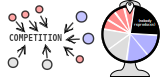
\includegraphics{images/roulette.png}

As can be seen, not all individual have the same size on the roulette
wheel. That depicts differences in their growth rates, biomass, or other
approximations of ``fitness''. Also, the roulette wheel contains an area
(shown in black) that shapes the chance that nobody reproduces. We will
try and implement this rule to let individuals reproduce based on their
fitness, but with only 10 competitors at a time. Let's start with a code
where individuals have a ``fitness'' value, but it not yet used for
selection (see below). \textbf{Read/test this code thoroughly before you
move on to the next section}.

\begin{tcolorbox}[enhanced jigsaw, left=2mm, opacitybacktitle=0.6, toptitle=1mm, colbacktitle=quarto-callout-note-color!10!white, toprule=.15mm, coltitle=black, colframe=quarto-callout-note-color-frame, opacityback=0, title=\textcolor{quarto-callout-note-color}{\faInfo}\hspace{0.5em}{CODE FOR ``fitness without fitness''}, breakable, bottomtitle=1mm, rightrule=.15mm, titlerule=0mm, arc=.35mm, leftrule=.75mm, bottomrule=.15mm, colback=white]

\begin{Shaded}
\begin{Highlighting}[]
\ImportTok{import}\NormalTok{ random}
\ImportTok{import}\NormalTok{ math}
\ImportTok{import}\NormalTok{ matplotlib.pyplot }\ImportTok{as}\NormalTok{ plt}

\CommentTok{\# Set the random number seed for reproducibility}
\NormalTok{random.seed(}\DecValTok{0}\NormalTok{)}

\NormalTok{plt.ion()  }\CommentTok{\# Enable interactive plotting}

\CommentTok{\# {-}{-}{-} PARAMETERS {-}{-}{-}}
\NormalTok{initial\_fitness }\OperatorTok{=} \FloatTok{0.1}            \CommentTok{\# Starting fitness for all individuals}
\NormalTok{population\_size }\OperatorTok{=} \DecValTok{500}             \CommentTok{\# Number of individuals (should be a square number for grid mode)}
\NormalTok{generations }\OperatorTok{=} \DecValTok{20000}               \CommentTok{\# Number of generations to simulate}
\NormalTok{mutation\_rate }\OperatorTok{=} \FloatTok{0.005}            \CommentTok{\# Probability of mutation per reproduction event}
\NormalTok{sample\_interval }\OperatorTok{=} \DecValTok{5}               \CommentTok{\# How often to sample and plot data}

\CommentTok{\# {-}{-}{-} INITIALIZATION {-}{-}{-}}
\CommentTok{\# Create initial population: all individuals start with the same fitness}
\NormalTok{population }\OperatorTok{=}\NormalTok{ [initial\_fitness }\ControlFlowTok{for}\NormalTok{ \_ }\KeywordTok{in} \BuiltInTok{range}\NormalTok{(population\_size)]}

\CommentTok{\# Lists to track average fitness and diversity over time}
\NormalTok{avg\_fitness }\OperatorTok{=}\NormalTok{ []}
\NormalTok{diversity\_over\_time }\OperatorTok{=}\NormalTok{ []}

\CommentTok{\# {-}{-}{-} CORE FUNCTIONS {-}{-}{-}}

\KeywordTok{def}\NormalTok{ mutate(fitness, rate}\OperatorTok{=}\NormalTok{mutation\_rate):}
    \CommentTok{"""Mutate the fitness value with a given probability."""}
    \ControlFlowTok{if}\NormalTok{ random.random() }\OperatorTok{\textless{}}\NormalTok{ rate:}
        \CommentTok{\# Fitness changes by a random value in [{-}0.1, 0.1], clipped to [0, 1]}
        \ControlFlowTok{return} \BuiltInTok{min}\NormalTok{(}\FloatTok{1.0}\NormalTok{, }\BuiltInTok{max}\NormalTok{(}\FloatTok{0.0}\NormalTok{, fitness }\OperatorTok{+}\NormalTok{ random.uniform(}\OperatorTok{{-}}\FloatTok{0.1}\NormalTok{, }\FloatTok{0.1}\NormalTok{)))}
    \ControlFlowTok{return}\NormalTok{ fitness}

\KeywordTok{def}\NormalTok{ calculate\_diversity(population):}
    \CommentTok{"""NOT YET IMPLEMENTED! Calculate diversity as the standard deviation of fitness values."""}
    \ControlFlowTok{return} \DecValTok{0} 

\CommentTok{\# {-}{-}{-} PLOTTING SETUP {-}{-}{-}}
\NormalTok{fig, ax1 }\OperatorTok{=}\NormalTok{ plt.subplots(figsize}\OperatorTok{=}\NormalTok{(}\DecValTok{12}\NormalTok{, }\DecValTok{8}\NormalTok{))}
\NormalTok{ax1.set\_xlabel(}\StringTok{"Generation"}\NormalTok{)}
\NormalTok{ax1.set\_ylabel(}\StringTok{"Average Fitness"}\NormalTok{, color}\OperatorTok{=}\StringTok{\textquotesingle{}tab:blue\textquotesingle{}}\NormalTok{)}
\NormalTok{ax1.set\_ylim(}\DecValTok{0}\NormalTok{, }\DecValTok{1}\NormalTok{)}
\NormalTok{line1, }\OperatorTok{=}\NormalTok{ ax1.plot([], [], color}\OperatorTok{=}\StringTok{\textquotesingle{}tab:blue\textquotesingle{}}\NormalTok{, linewidth}\OperatorTok{=}\DecValTok{2}\NormalTok{, label}\OperatorTok{=}\StringTok{\textquotesingle{}Fitness\textquotesingle{}}\NormalTok{)}
\NormalTok{ax1.tick\_params(axis}\OperatorTok{=}\StringTok{\textquotesingle{}y\textquotesingle{}}\NormalTok{, labelcolor}\OperatorTok{=}\StringTok{\textquotesingle{}tab:blue\textquotesingle{}}\NormalTok{)}

\CommentTok{\# Second y{-}axis for diversity}
\NormalTok{ax2 }\OperatorTok{=}\NormalTok{ ax1.twinx()}
\NormalTok{ax2.set\_ylabel(}\StringTok{"Diversity"}\NormalTok{, color}\OperatorTok{=}\StringTok{\textquotesingle{}tab:green\textquotesingle{}}\NormalTok{)}
\NormalTok{line2, }\OperatorTok{=}\NormalTok{ ax2.plot([], [], color}\OperatorTok{=}\StringTok{\textquotesingle{}tab:green\textquotesingle{}}\NormalTok{, linestyle}\OperatorTok{=}\StringTok{\textquotesingle{}:\textquotesingle{}}\NormalTok{, linewidth}\OperatorTok{=}\DecValTok{2}\NormalTok{, label}\OperatorTok{=}\StringTok{\textquotesingle{}Diversity\textquotesingle{}}\NormalTok{)}
\NormalTok{ax2.tick\_params(axis}\OperatorTok{=}\StringTok{\textquotesingle{}y\textquotesingle{}}\NormalTok{, labelcolor}\OperatorTok{=}\StringTok{\textquotesingle{}tab:green\textquotesingle{}}\NormalTok{)}

\NormalTok{fig.suptitle(}\StringTok{"Evolution Toward Fitness 1"}\NormalTok{)}
\NormalTok{fig.tight\_layout()}
\NormalTok{fig.legend(loc}\OperatorTok{=}\StringTok{\textquotesingle{}upper right\textquotesingle{}}\NormalTok{)}
\NormalTok{plt.grid(}\VariableTok{True}\NormalTok{)}
\NormalTok{plt.draw()}

\CommentTok{\# {-}{-}{-} EVOLUTION LOOP {-}{-}{-}}
\NormalTok{best\_fitness }\OperatorTok{=} \OperatorTok{{-}}\DecValTok{1}
\NormalTok{found }\OperatorTok{=} \VariableTok{False}

\ControlFlowTok{for}\NormalTok{ gen }\KeywordTok{in} \BuiltInTok{range}\NormalTok{(generations):}
\NormalTok{    total\_fit }\OperatorTok{=} \BuiltInTok{sum}\NormalTok{(population)}
\NormalTok{    best }\OperatorTok{=} \BuiltInTok{max}\NormalTok{(population)}
    \CommentTok{\# Print when a perfect solution is found}
    \ControlFlowTok{if}\NormalTok{ best }\OperatorTok{==} \DecValTok{1} \KeywordTok{and} \KeywordTok{not}\NormalTok{ found:}
\NormalTok{        found }\OperatorTok{=} \VariableTok{True}
        \BuiltInTok{print}\NormalTok{(}\StringTok{"Found perfect solution at generation"}\NormalTok{, gen)}
        
    \CommentTok{\# Sample and plot data at intervals}
    \ControlFlowTok{if}\NormalTok{ gen }\OperatorTok{\%}\NormalTok{ sample\_interval }\OperatorTok{==} \DecValTok{0}\NormalTok{:}
\NormalTok{        avg\_fitness.append(total\_fit }\OperatorTok{/}\NormalTok{ population\_size)}
\NormalTok{        diversity\_over\_time.append(calculate\_diversity(population))}
\NormalTok{        x\_vals }\OperatorTok{=}\NormalTok{ [i }\OperatorTok{*}\NormalTok{ sample\_interval }\ControlFlowTok{for}\NormalTok{ i }\KeywordTok{in} \BuiltInTok{range}\NormalTok{(}\BuiltInTok{len}\NormalTok{(avg\_fitness))]}
\NormalTok{        line1.set\_data(x\_vals, avg\_fitness)}
\NormalTok{        line2.set\_data(x\_vals, diversity\_over\_time)}
\NormalTok{        ax1.relim()}\OperatorTok{;}\NormalTok{ ax1.autoscale\_view()}
\NormalTok{        ax2.relim()}\OperatorTok{;}\NormalTok{ ax2.autoscale\_view()}
\NormalTok{        fig.suptitle(}\SpecialStringTok{f"Best Fitness: }\SpecialCharTok{\{}\NormalTok{best}\SpecialCharTok{:.2f\}}\SpecialStringTok{"}\NormalTok{, fontsize}\OperatorTok{=}\DecValTok{14}\NormalTok{)}
\NormalTok{        plt.pause(}\FloatTok{0.01}\NormalTok{)}
        

    \CommentTok{\# {-}{-}{-} MORAN PROCESS {-}{-}{-}}
    \CommentTok{\# For each individual, perform a reproduction event}
    \ControlFlowTok{for}\NormalTok{ \_ }\KeywordTok{in} \BuiltInTok{range}\NormalTok{(}\DecValTok{100}\NormalTok{):  }\CommentTok{\# 100 competition events per generation}
        \CommentTok{\# Select 1 random individual for replication}
\NormalTok{        probs }\OperatorTok{=}\NormalTok{ [}\DecValTok{1} \ControlFlowTok{for}\NormalTok{ fit }\KeywordTok{in}\NormalTok{ population] }\CommentTok{\# All probability weights are equal (1.0)}
\NormalTok{        parent\_idx }\OperatorTok{=}\NormalTok{ random.choices(}\BuiltInTok{range}\NormalTok{(}\BuiltInTok{len}\NormalTok{(population)), weights}\OperatorTok{=}\NormalTok{probs)[}\DecValTok{0}\NormalTok{] }\CommentTok{\# Grab one random individual based on an unweighted list...}
        \CommentTok{\# Select individual to be replaced (uniform random)}
\NormalTok{        dead\_idx }\OperatorTok{=}\NormalTok{ random.randrange(}\BuiltInTok{len}\NormalTok{(population))}
        \CommentTok{\# Copy population for next generation}
\NormalTok{        new\_pop }\OperatorTok{=}\NormalTok{ population.copy()}
        \CommentTok{\# Offspring replaces the dead individual (with possible mutation)}
\NormalTok{        new\_pop[dead\_idx] }\OperatorTok{=}\NormalTok{ mutate(population[parent\_idx])}
\NormalTok{        population }\OperatorTok{=}\NormalTok{ new\_pop}

\BuiltInTok{input}\NormalTok{(}\StringTok{"}\CharTok{\textbackslash{}n}\StringTok{Simulation complete. Press Enter to exit plot window..."}\NormalTok{)}
\end{Highlighting}
\end{Shaded}

\end{tcolorbox}

\section{Making a roulette wheel with everyone in
it}\label{making-a-roulette-wheel-with-everyone-in-it}

If you have read the code, you will see that we can pass a list of
weights to the function \texttt{random.choices}, to determine who is
most likely to be sampled. Currently, all the weights are set to 1:

\texttt{probs\ =\ {[}1\ for\ fit\ in\ population{]}\ \#\ All\ probability\ weights\ are\ equal\ (1.0)}

\begin{enumerate}
\def\labelenumi{\alph{enumi}.}
\tightlist
\item
  Run the code with the current (all equal) weights. What happens?
\item
  Modify this line of code to take the fitness values as the weight,
  rather than 1. (hint: this is a VERY small change in the code).
\end{enumerate}

\section{A roulette wheel of a subset of
individuals}\label{a-roulette-wheel-of-a-subset-of-individuals}

Instead of letting everyone reproduce, let us modify the code to only
sample from a smaller list of `competitors', and spin a virtual roulette
wheel to determine who wins. There are many ways to implement this, but
here's how we will do it. We will sample N individuals from the
population, and implement the following algorithm:

\begin{enumerate}
\def\labelenumi{\arabic{enumi}.}
\tightlist
\item
  Select a random subset of N individuals from the population.
\item
  Take/compute the fitness of each selected individual.
\item
  Add a reproduction-skip option with a fixed weight.
\item
  Choose one individual or the skip option using weighted random
  selection.
\item
  If an individual was chosen, mutate it and replace a random individual
  in the population.
\end{enumerate}

Below, there's a small snippet of code doing what is explained
above\footnote{Note that this is from the full code, so this code does
  not work stand-alone}. The variable \texttt{no\_reproduction\_chance}
is the fixed weight that nobody gets to reproduce:

\begin{tcolorbox}[enhanced jigsaw, left=2mm, opacitybacktitle=0.6, toptitle=1mm, colbacktitle=quarto-callout-note-color!10!white, toprule=.15mm, coltitle=black, colframe=quarto-callout-note-color-frame, opacityback=0, title=\textcolor{quarto-callout-note-color}{\faInfo}\hspace{0.5em}{Roulette wheel algorithm}, breakable, bottomtitle=1mm, rightrule=.15mm, titlerule=0mm, arc=.35mm, leftrule=.75mm, bottomrule=.15mm, colback=white]

\begin{Shaded}
\begin{Highlighting}[]
\NormalTok{  tournament\_size }\OperatorTok{=} \DecValTok{10}  
\NormalTok{  no\_reproduction\_chance }\OperatorTok{=} \DecValTok{1}
  
\NormalTok{  competitors }\OperatorTok{=}\NormalTok{ random.sample(population, tournament\_size)}
  \CommentTok{\# Make a list of their fitness values}
\NormalTok{  fitness\_values }\OperatorTok{=}\NormalTok{ [fit }\ControlFlowTok{for}\NormalTok{ fit }\KeywordTok{in}\NormalTok{ competitors]}
\NormalTok{  total }\OperatorTok{=} \BuiltInTok{sum}\NormalTok{(fitness\_values)}
  \CommentTok{\# Add a "no reproduction" dummy competitor with fitness = 0}
\NormalTok{  competitors\_with\_dummy }\OperatorTok{=}\NormalTok{ competitors }\OperatorTok{+}\NormalTok{ [}\VariableTok{None}\NormalTok{]}
\NormalTok{  probs }\OperatorTok{=}\NormalTok{ [f }\OperatorTok{/}\NormalTok{ total }\ControlFlowTok{for}\NormalTok{ f }\KeywordTok{in}\NormalTok{ fitness\_values] }\OperatorTok{+}\NormalTok{ [no\_reproduction\_chance]}
\NormalTok{  winner }\OperatorTok{=}\NormalTok{ random.choices(competitors\_with\_dummy, weights}\OperatorTok{=}\NormalTok{probs, k}\OperatorTok{=}\DecValTok{1}\NormalTok{)[}\DecValTok{0}\NormalTok{]}
  \ControlFlowTok{if}\NormalTok{ winner }\KeywordTok{is} \KeywordTok{not} \VariableTok{None}\NormalTok{:}
      \CommentTok{\# Mutate winner to produce offspring}
\NormalTok{      offspring }\OperatorTok{=}\NormalTok{ mutate(winner)}
\NormalTok{      remove\_idx }\OperatorTok{=}\NormalTok{ random.randrange(}\BuiltInTok{len}\NormalTok{(population))}
\NormalTok{      population[remove\_idx] }\OperatorTok{=}\NormalTok{ offspring  }
        
\end{Highlighting}
\end{Shaded}

\end{tcolorbox}

After you understand the roulette wheel algorithm, do the following
exercise:

\begin{exercise}[Questions about the roulette wheel - Algorithmic
thinking]\protect\hypertarget{exr-roulette}{}\label{exr-roulette}

\begin{enumerate}
\def\labelenumi{\alph{enumi}.}
\tightlist
\item
  Let's imagine a moment where the roulette wheel contains only 10
  highly unfit individuals (e.g.~all fitness values are 0.01). What is
  the chance that someone will reproduce? (you don't have to calculate
  it, but give your reasoning)
\item
  Answer the same question as in \textbf{a.}, but now imagine that all
  10 individuals have a fitness value of 1.
\item
  Answer question b. and c.~again, but now assume that
  \texttt{no\_reproduction\_chance} is equal to 0.
\item
  Describe what the \texttt{no\_reproduction\_chance} parameter does in
  biological terms.
\item
  Spatially structured populations are often placed on a grid.
  \textbf{Describe} how you could implement a roulette wheel to resolve
  \emph{local} competition, \emph{e.g.} when an empty grid point is
  competed for by the neighbours.
\end{enumerate}

\end{exercise}

\section{Diversity patterns}\label{diversity-patterns}

Modify the function \texttt{calculate\_diversity} to calculate the
diversity of the population as the standard deviation of the fitness
values.

\begin{exercise}[The dynamics of diversity -
Biology]\protect\hypertarget{exr-diversitydynamics}{}\label{exr-diversitydynamics}

\begin{enumerate}
\def\labelenumi{\alph{enumi}.}
\tightlist
\item
  Use a low mutation rate and study the dynamics of diversity. Describe
  the pattern verbally.
\end{enumerate}

\end{exercise}

\section{Evolving a DNA sequence}\label{evolving-a-dna-sequence}

A big problem with the previous model is there is no true distinction
between genotype (that which mutates) and phenotype (that which is
selected). Let us try and adapt the model to be more biologically
meaningful, by making each individual represented by a DNA sequence.
Copy the following code:

\begin{tcolorbox}[enhanced jigsaw, left=2mm, opacitybacktitle=0.6, toptitle=1mm, colbacktitle=quarto-callout-note-color!10!white, toprule=.15mm, coltitle=black, colframe=quarto-callout-note-color-frame, opacityback=0, title=\textcolor{quarto-callout-note-color}{\faInfo}\hspace{0.5em}{Starting code for ``evolving a DNA sequence''}, breakable, bottomtitle=1mm, rightrule=.15mm, titlerule=0mm, arc=.35mm, leftrule=.75mm, bottomrule=.15mm, colback=white]

\begin{Shaded}
\begin{Highlighting}[]
\ImportTok{import}\NormalTok{ random}
\ImportTok{import}\NormalTok{ math}
\ImportTok{import}\NormalTok{ matplotlib.pyplot }\ImportTok{as}\NormalTok{ plt}
\ImportTok{from}\NormalTok{ collections }\ImportTok{import}\NormalTok{ Counter}

\CommentTok{\# set the random number seed}
\NormalTok{random.seed(}\DecValTok{0}\NormalTok{)}

\NormalTok{plt.ion()  }\CommentTok{\# Enable interactive mode}

\CommentTok{\# Parameters}
\NormalTok{alphabet }\OperatorTok{=} \StringTok{"ATCG"}
\NormalTok{target\_sequence }\OperatorTok{=} \StringTok{"GATGCGCGCTGGATTAAC"}  \CommentTok{\# Example target sequence}
\NormalTok{dna\_length }\OperatorTok{=} \BuiltInTok{len}\NormalTok{(target\_sequence)}
\NormalTok{target\_length }\OperatorTok{=} \BuiltInTok{len}\NormalTok{(target\_sequence)}

\CommentTok{\# Simulation settings}
\NormalTok{population\_size }\OperatorTok{=} \DecValTok{500}  \CommentTok{\# must be a square number for grid mode}
\NormalTok{generations }\OperatorTok{=} \DecValTok{20000}
\NormalTok{mutation\_rate }\OperatorTok{=} \FloatTok{0.001}
\NormalTok{sample\_interval }\OperatorTok{=} \DecValTok{5}
\NormalTok{sample\_size }\OperatorTok{=}\NormalTok{ population\_size}
\NormalTok{no\_reproduction\_chance }\OperatorTok{=} \FloatTok{0.1}

\CommentTok{\# Core functions}
\KeywordTok{def}\NormalTok{ fitness(dna):}
    \ControlFlowTok{return} \DecValTok{1} \OperatorTok{{-}} \BuiltInTok{sum}\NormalTok{(a }\OperatorTok{!=}\NormalTok{ b }\ControlFlowTok{for}\NormalTok{ a, b }\KeywordTok{in} \BuiltInTok{zip}\NormalTok{(dna, target\_sequence)) }\OperatorTok{/}\NormalTok{ target\_length}

\KeywordTok{def}\NormalTok{ mutate(dna, rate}\OperatorTok{=}\NormalTok{mutation\_rate):}
    \ControlFlowTok{return} \StringTok{\textquotesingle{}\textquotesingle{}}\NormalTok{.join(}
\NormalTok{        random.choice([b }\ControlFlowTok{for}\NormalTok{ b }\KeywordTok{in}\NormalTok{ alphabet }\ControlFlowTok{if}\NormalTok{ b }\OperatorTok{!=}\NormalTok{ base]) }\ControlFlowTok{if}\NormalTok{ random.random() }\OperatorTok{\textless{}}\NormalTok{ rate }\ControlFlowTok{else}\NormalTok{ base}
        \ControlFlowTok{for}\NormalTok{ base }\KeywordTok{in}\NormalTok{ dna}
\NormalTok{    )}

\KeywordTok{def}\NormalTok{ count\_beneficial\_mutations(dna):}
\NormalTok{    f0 }\OperatorTok{=}\NormalTok{ fitness(dna)}
\NormalTok{    count }\OperatorTok{=} \DecValTok{0}
    \ControlFlowTok{for}\NormalTok{ i }\KeywordTok{in} \BuiltInTok{range}\NormalTok{(}\BuiltInTok{len}\NormalTok{(dna)):}
        \ControlFlowTok{for}\NormalTok{ b }\KeywordTok{in}\NormalTok{ alphabet:}
            \ControlFlowTok{if}\NormalTok{ b }\OperatorTok{!=}\NormalTok{ dna[i]:}
\NormalTok{                mutant }\OperatorTok{=}\NormalTok{ dna[:i] }\OperatorTok{+}\NormalTok{ b }\OperatorTok{+}\NormalTok{ dna[i}\OperatorTok{+}\DecValTok{1}\NormalTok{:]}
                \ControlFlowTok{if}\NormalTok{ fitness(mutant) }\OperatorTok{\textgreater{}}\NormalTok{ f0:}
\NormalTok{                    count }\OperatorTok{+=} \DecValTok{1}
    \ControlFlowTok{return}\NormalTok{ count}

\KeywordTok{def}\NormalTok{ diversity(pop):}
\NormalTok{    counts }\OperatorTok{=}\NormalTok{ \{\}}
    \ControlFlowTok{for}\NormalTok{ ind }\KeywordTok{in}\NormalTok{ pop:}
\NormalTok{        counts[ind] }\OperatorTok{=}\NormalTok{ counts.get(ind, }\DecValTok{0}\NormalTok{) }\OperatorTok{+} \DecValTok{1}
\NormalTok{    total }\OperatorTok{=} \BuiltInTok{len}\NormalTok{(pop)}
    \ControlFlowTok{return} \OperatorTok{{-}}\BuiltInTok{sum}\NormalTok{((c}\OperatorTok{/}\NormalTok{total) }\OperatorTok{*}\NormalTok{ math.log(c}\OperatorTok{/}\NormalTok{total }\OperatorTok{+} \FloatTok{1e{-}9}\NormalTok{) }\ControlFlowTok{for}\NormalTok{ c }\KeywordTok{in}\NormalTok{ counts.values()) }\ControlFlowTok{if}\NormalTok{ total }\OperatorTok{\textgreater{}} \DecValTok{0} \ControlFlowTok{else} \DecValTok{0}

\CommentTok{\# Initialize population}
\NormalTok{initial\_sequence }\OperatorTok{=} \StringTok{"GATAGCGAAGTTTAGCCG"} \CommentTok{\# far from target (only first 3 are correct)}
\NormalTok{population }\OperatorTok{=}\NormalTok{ [initial\_sequence }\ControlFlowTok{for}\NormalTok{ \_ }\KeywordTok{in} \BuiltInTok{range}\NormalTok{(population\_size)]}

\NormalTok{avg\_fitness }\OperatorTok{=}\NormalTok{ []}
\NormalTok{avg\_beneficial }\OperatorTok{=}\NormalTok{ []}
\NormalTok{diversity\_over\_time }\OperatorTok{=}\NormalTok{ []}
\NormalTok{best\_individuals }\OperatorTok{=}\NormalTok{ []}

\KeywordTok{def}\NormalTok{ get\_neighbors(i, j):}
    \ControlFlowTok{return}\NormalTok{ [(x }\OperatorTok{\%}\NormalTok{ side, y }\OperatorTok{\%}\NormalTok{ side)}
            \ControlFlowTok{for}\NormalTok{ x }\KeywordTok{in} \BuiltInTok{range}\NormalTok{(i}\OperatorTok{{-}}\DecValTok{1}\NormalTok{, i}\OperatorTok{+}\DecValTok{2}\NormalTok{)}
            \ControlFlowTok{for}\NormalTok{ y }\KeywordTok{in} \BuiltInTok{range}\NormalTok{(j}\OperatorTok{{-}}\DecValTok{1}\NormalTok{, j}\OperatorTok{+}\DecValTok{2}\NormalTok{)]}

\CommentTok{\# Initialize interactive plot}
\NormalTok{fig, ax1 }\OperatorTok{=}\NormalTok{ plt.subplots(figsize}\OperatorTok{=}\NormalTok{(}\DecValTok{12}\NormalTok{, }\DecValTok{8}\NormalTok{))}
\NormalTok{ax1.set\_xlabel(}\StringTok{"Generation"}\NormalTok{)}
\NormalTok{ax1.set\_ylabel(}\StringTok{"Average Fitness"}\NormalTok{, color}\OperatorTok{=}\StringTok{\textquotesingle{}tab:blue\textquotesingle{}}\NormalTok{)}
\NormalTok{ax1.set\_ylim(}\DecValTok{0}\NormalTok{, }\DecValTok{1}\NormalTok{)}
\NormalTok{line1, }\OperatorTok{=}\NormalTok{ ax1.plot([], [], color}\OperatorTok{=}\StringTok{\textquotesingle{}tab:blue\textquotesingle{}}\NormalTok{, linewidth}\OperatorTok{=}\DecValTok{2}\NormalTok{, label}\OperatorTok{=}\StringTok{\textquotesingle{}Fitness\textquotesingle{}}\NormalTok{)}
\NormalTok{ax1.tick\_params(axis}\OperatorTok{=}\StringTok{\textquotesingle{}y\textquotesingle{}}\NormalTok{, labelcolor}\OperatorTok{=}\StringTok{\textquotesingle{}tab:blue\textquotesingle{}}\NormalTok{)}

\NormalTok{ax2 }\OperatorTok{=}\NormalTok{ ax1.twinx()}
\NormalTok{ax2.set\_ylabel(}\StringTok{"Beneficial Mutations / Diversity"}\NormalTok{, color}\OperatorTok{=}\StringTok{\textquotesingle{}tab:purple\textquotesingle{}}\NormalTok{)}
\NormalTok{line2, }\OperatorTok{=}\NormalTok{ ax2.plot([], [], color}\OperatorTok{=}\StringTok{\textquotesingle{}tab:purple\textquotesingle{}}\NormalTok{, linestyle}\OperatorTok{=}\StringTok{\textquotesingle{}{-}{-}\textquotesingle{}}\NormalTok{, linewidth}\OperatorTok{=}\DecValTok{2}\NormalTok{, label}\OperatorTok{=}\StringTok{\textquotesingle{}Beneficial Mutations\textquotesingle{}}\NormalTok{)}
\NormalTok{line3, }\OperatorTok{=}\NormalTok{ ax2.plot([], [], color}\OperatorTok{=}\StringTok{\textquotesingle{}tab:green\textquotesingle{}}\NormalTok{, linestyle}\OperatorTok{=}\StringTok{\textquotesingle{}:\textquotesingle{}}\NormalTok{, linewidth}\OperatorTok{=}\DecValTok{2}\NormalTok{, label}\OperatorTok{=}\StringTok{\textquotesingle{}Diversity\textquotesingle{}}\NormalTok{)}
\NormalTok{ax2.tick\_params(axis}\OperatorTok{=}\StringTok{\textquotesingle{}y\textquotesingle{}}\NormalTok{, labelcolor}\OperatorTok{=}\StringTok{\textquotesingle{}tab:purple\textquotesingle{}}\NormalTok{)}
\NormalTok{fig.suptitle(}\StringTok{"Evolution Toward Target Sequence"}\NormalTok{)}
\NormalTok{fig.tight\_layout()}
\NormalTok{ax2.set\_ylim(}\DecValTok{0}\NormalTok{, }\DecValTok{20}\NormalTok{)}
\NormalTok{fig.legend(loc}\OperatorTok{=}\StringTok{\textquotesingle{}upper right\textquotesingle{}}\NormalTok{)}
\NormalTok{plt.grid(}\VariableTok{True}\NormalTok{)}
\NormalTok{plt.draw()}

\NormalTok{best\_seq }\OperatorTok{=} \StringTok{""}
\NormalTok{best\_score }\OperatorTok{=} \OperatorTok{{-}}\DecValTok{1}
\NormalTok{found }\OperatorTok{=} \VariableTok{False}

\CommentTok{\# Evolution loop}
\ControlFlowTok{for}\NormalTok{ gen }\KeywordTok{in} \BuiltInTok{range}\NormalTok{(generations):}
\NormalTok{    fitnesses }\OperatorTok{=}\NormalTok{ [fitness(ind) }\ControlFlowTok{for}\NormalTok{ ind }\KeywordTok{in}\NormalTok{ population]}
\NormalTok{    total\_fit }\OperatorTok{=} \BuiltInTok{sum}\NormalTok{(fitnesses)}
\NormalTok{    best }\OperatorTok{=} \BuiltInTok{max}\NormalTok{(fitnesses)}
    \ControlFlowTok{if}\NormalTok{(best }\OperatorTok{==} \DecValTok{1} \KeywordTok{and} \KeywordTok{not}\NormalTok{ found):}
\NormalTok{        found }\OperatorTok{=} \VariableTok{True}
        \BuiltInTok{print}\NormalTok{(}\StringTok{"Found perfect solution at generation"}\NormalTok{, gen)}
        
    \ControlFlowTok{if}\NormalTok{ gen }\OperatorTok{\%}\NormalTok{ sample\_interval }\OperatorTok{==} \DecValTok{0}\NormalTok{:}
\NormalTok{        sample }\OperatorTok{=}\NormalTok{ random.sample(population, sample\_size)}
\NormalTok{        avg\_beneficial.append(}\BuiltInTok{sum}\NormalTok{(count\_beneficial\_mutations(ind) }\ControlFlowTok{for}\NormalTok{ ind }\KeywordTok{in}\NormalTok{ sample) }\OperatorTok{/}\NormalTok{ sample\_size)}
\NormalTok{        diversity\_over\_time.append(diversity(population))}

        \CommentTok{\# Update plot data}
\NormalTok{        line1.set\_data(}\BuiltInTok{range}\NormalTok{(}\BuiltInTok{len}\NormalTok{(avg\_fitness)}\OperatorTok{+}\DecValTok{1}\NormalTok{), avg\_fitness }\OperatorTok{+}\NormalTok{ [}\BuiltInTok{sum}\NormalTok{(fitnesses)}\OperatorTok{/}\NormalTok{population\_size])}
\NormalTok{        line2.set\_data(}\BuiltInTok{range}\NormalTok{(}\BuiltInTok{len}\NormalTok{(avg\_beneficial)), avg\_beneficial)}
\NormalTok{        line3.set\_data(}\BuiltInTok{range}\NormalTok{(}\BuiltInTok{len}\NormalTok{(diversity\_over\_time)), diversity\_over\_time)}
\NormalTok{        ax1.relim()}\OperatorTok{;}\NormalTok{ ax1.autoscale\_view()}
\NormalTok{        ax2.relim()}\OperatorTok{;}\NormalTok{ ax2.autoscale\_view()}
\NormalTok{        best }\OperatorTok{=} \BuiltInTok{max}\NormalTok{(population, key}\OperatorTok{=}\NormalTok{fitness)}
\NormalTok{        fig.suptitle(}\SpecialStringTok{f"Best: }\SpecialCharTok{\{}\NormalTok{best}\SpecialCharTok{\}}\SpecialStringTok{ (target: }\SpecialCharTok{\{}\NormalTok{target\_sequence}\SpecialCharTok{\}}\SpecialStringTok{)"}\NormalTok{, fontsize}\OperatorTok{=}\DecValTok{14}\NormalTok{)}
\NormalTok{        plt.pause(}\FloatTok{0.01}\NormalTok{)}

    \ControlFlowTok{else}\NormalTok{:}
\NormalTok{        avg\_beneficial.append(avg\_beneficial[}\OperatorTok{{-}}\DecValTok{1}\NormalTok{])}
\NormalTok{        diversity\_over\_time.append(diversity\_over\_time[}\OperatorTok{{-}}\DecValTok{1}\NormalTok{])}

    \CommentTok{\# Tournament selection (as in evolving\_fitness\_final.py)}
\NormalTok{    new\_pop }\OperatorTok{=}\NormalTok{ []}
\NormalTok{    tournament\_size }\OperatorTok{=} \DecValTok{10}  \CommentTok{\# can be adjusted}

    \ControlFlowTok{for}\NormalTok{ \_ }\KeywordTok{in} \BuiltInTok{range}\NormalTok{(population\_size):}
        \CommentTok{\# Select tournament\_size individuals randomly}
\NormalTok{        competitors }\OperatorTok{=}\NormalTok{ random.sample(population, tournament\_size)}
        \CommentTok{\# Pick the one with highest fitness}
\NormalTok{        fitness\_values }\OperatorTok{=}\NormalTok{ [fitness(ind) }\ControlFlowTok{for}\NormalTok{ ind }\KeywordTok{in}\NormalTok{ competitors]}
\NormalTok{        total }\OperatorTok{=} \BuiltInTok{sum}\NormalTok{(fitness\_values)}
        
\NormalTok{        probs }\OperatorTok{=}\NormalTok{ [f }\OperatorTok{/}\NormalTok{ total }\ControlFlowTok{for}\NormalTok{ f }\KeywordTok{in}\NormalTok{ fitness\_values]}
\NormalTok{        winner }\OperatorTok{=}\NormalTok{ random.choices(competitors, weights}\OperatorTok{=}\NormalTok{probs, k}\OperatorTok{=}\DecValTok{1}\NormalTok{)[}\DecValTok{0}\NormalTok{]}
        \CommentTok{\# Mutate winner to produce offspring}
\NormalTok{        offspring }\OperatorTok{=}\NormalTok{ mutate(winner)}
\NormalTok{        new\_pop.append(offspring)}

\NormalTok{    population }\OperatorTok{=}\NormalTok{ new\_pop}

\NormalTok{    avg\_fitness.append(}\BuiltInTok{sum}\NormalTok{(fitness(ind) }\ControlFlowTok{for}\NormalTok{ ind }\KeywordTok{in}\NormalTok{ population) }\OperatorTok{/}\NormalTok{ population\_size)}
    \ControlFlowTok{if}\NormalTok{ gen }\OperatorTok{\%} \DecValTok{250} \OperatorTok{==} \DecValTok{0}\NormalTok{:}
\NormalTok{        best }\OperatorTok{=} \BuiltInTok{max}\NormalTok{(population, key}\OperatorTok{=}\NormalTok{fitness)}
\NormalTok{        best\_individuals.append((gen, best))}

\BuiltInTok{input}\NormalTok{(}\StringTok{"}\CharTok{\textbackslash{}n}\StringTok{Simulation complete. Press Enter to exit plot window..."}\NormalTok{)}
\end{Highlighting}
\end{Shaded}

\end{tcolorbox}

Answer the following questions using the options available in the model:

\begin{exercise}[Evolving DNA - Biology / abstract
thinking]\protect\hypertarget{exr-evolving-dna}{}\label{exr-evolving-dna}

~

\begin{enumerate}
\def\labelenumi{\alph{enumi}.}
\tightlist
\item
  Run the code. What does the new (dashed blue) line represent? Do you
  understand how is changes over time?
\end{enumerate}

The program reports after how many generations it manages to find the
target sequence. With default settings this can take a long time\ldots{}
(default: 4633 generations)

\begin{enumerate}
\def\labelenumi{\alph{enumi}.}
\setcounter{enumi}{1}
\tightlist
\item
  Modify the mutation rate to see how it affects the time to find the
  target sequence. Try different mutation rates between 0.0001 and 0.1.
  Keep track of both how long (number of generations) it takes to find
  the target, and how fit the population is once the target is found.
  What do you observe?
\item
  Diversity is no longer calculated as the standard deviation in
  fitness, but as the Shannon diversity of all present sequences
  (although it is not super complex, you do not need to fully understand
  this function). Because of this, the exact number (quantities) cannot
  be compared to our ealrier model. Do you see a \emph{qualitative}
  differences?
\item
  Study how fitness is calculated in this model. Is there a distinction
  between genotype en phenotype? Why/why not?
\end{enumerate}

\end{exercise}

\section{Evolving a protein sequence}\label{evolving-a-protein-sequence}

Next we will extend the simulation a little more. The individual
genotypes will still be represented as a DNA sequence, but before
evaluating fitness this will be translated into a \textbf{protein}
sequence. To do so, the code first defines the codon table (which we of
course all know by heart =)), and then translates the DNA sequence into
a protein sequence. The protein sequence is then used to calculate the
fitness of the individual, which is based on how well the protein
sequence matches a target protein sequence. The code is as follows:

\begin{tcolorbox}[enhanced jigsaw, left=2mm, opacitybacktitle=0.6, toptitle=1mm, colbacktitle=quarto-callout-note-color!10!white, toprule=.15mm, coltitle=black, colframe=quarto-callout-note-color-frame, opacityback=0, title=\textcolor{quarto-callout-note-color}{\faInfo}\hspace{0.5em}{Starting code for evolving a protein sequence}, breakable, bottomtitle=1mm, rightrule=.15mm, titlerule=0mm, arc=.35mm, leftrule=.75mm, bottomrule=.15mm, colback=white]

\begin{Shaded}
\begin{Highlighting}[]
\ImportTok{import}\NormalTok{ random}
\ImportTok{import}\NormalTok{ math}
\ImportTok{import}\NormalTok{ matplotlib.pyplot }\ImportTok{as}\NormalTok{ plt}
\ImportTok{from}\NormalTok{ collections }\ImportTok{import}\NormalTok{ Counter}

\CommentTok{\# set the random number seed}
\NormalTok{random.seed(}\DecValTok{0}\NormalTok{)}

\NormalTok{plt.ion()  }\CommentTok{\# Enable interactive mode}

\CommentTok{\# Codon table}
\NormalTok{codon\_table }\OperatorTok{=}\NormalTok{ \{}
    \StringTok{\textquotesingle{}TTT\textquotesingle{}}\NormalTok{: }\StringTok{\textquotesingle{}F\textquotesingle{}}\NormalTok{, }\StringTok{\textquotesingle{}TTC\textquotesingle{}}\NormalTok{: }\StringTok{\textquotesingle{}F\textquotesingle{}}\NormalTok{, }\StringTok{\textquotesingle{}TTA\textquotesingle{}}\NormalTok{: }\StringTok{\textquotesingle{}L\textquotesingle{}}\NormalTok{, }\StringTok{\textquotesingle{}TTG\textquotesingle{}}\NormalTok{: }\StringTok{\textquotesingle{}L\textquotesingle{}}\NormalTok{, }\StringTok{\textquotesingle{}CTT\textquotesingle{}}\NormalTok{: }\StringTok{\textquotesingle{}L\textquotesingle{}}\NormalTok{, }\StringTok{\textquotesingle{}CTC\textquotesingle{}}\NormalTok{: }\StringTok{\textquotesingle{}L\textquotesingle{}}\NormalTok{, }\StringTok{\textquotesingle{}CTA\textquotesingle{}}\NormalTok{: }\StringTok{\textquotesingle{}L\textquotesingle{}}\NormalTok{, }\StringTok{\textquotesingle{}CTG\textquotesingle{}}\NormalTok{: }\StringTok{\textquotesingle{}L\textquotesingle{}}\NormalTok{,}
    \StringTok{\textquotesingle{}ATT\textquotesingle{}}\NormalTok{: }\StringTok{\textquotesingle{}I\textquotesingle{}}\NormalTok{, }\StringTok{\textquotesingle{}ATC\textquotesingle{}}\NormalTok{: }\StringTok{\textquotesingle{}I\textquotesingle{}}\NormalTok{, }\StringTok{\textquotesingle{}ATA\textquotesingle{}}\NormalTok{: }\StringTok{\textquotesingle{}I\textquotesingle{}}\NormalTok{, }\StringTok{\textquotesingle{}ATG\textquotesingle{}}\NormalTok{: }\StringTok{\textquotesingle{}M\textquotesingle{}}\NormalTok{,}
    \StringTok{\textquotesingle{}GTT\textquotesingle{}}\NormalTok{: }\StringTok{\textquotesingle{}V\textquotesingle{}}\NormalTok{, }\StringTok{\textquotesingle{}GTC\textquotesingle{}}\NormalTok{: }\StringTok{\textquotesingle{}V\textquotesingle{}}\NormalTok{, }\StringTok{\textquotesingle{}GTA\textquotesingle{}}\NormalTok{: }\StringTok{\textquotesingle{}V\textquotesingle{}}\NormalTok{, }\StringTok{\textquotesingle{}GTG\textquotesingle{}}\NormalTok{: }\StringTok{\textquotesingle{}V\textquotesingle{}}\NormalTok{,}
    \StringTok{\textquotesingle{}TCT\textquotesingle{}}\NormalTok{: }\StringTok{\textquotesingle{}S\textquotesingle{}}\NormalTok{, }\StringTok{\textquotesingle{}TCC\textquotesingle{}}\NormalTok{: }\StringTok{\textquotesingle{}S\textquotesingle{}}\NormalTok{, }\StringTok{\textquotesingle{}TCA\textquotesingle{}}\NormalTok{: }\StringTok{\textquotesingle{}S\textquotesingle{}}\NormalTok{, }\StringTok{\textquotesingle{}TCG\textquotesingle{}}\NormalTok{: }\StringTok{\textquotesingle{}S\textquotesingle{}}\NormalTok{, }\StringTok{\textquotesingle{}AGT\textquotesingle{}}\NormalTok{: }\StringTok{\textquotesingle{}S\textquotesingle{}}\NormalTok{, }\StringTok{\textquotesingle{}AGC\textquotesingle{}}\NormalTok{: }\StringTok{\textquotesingle{}S\textquotesingle{}}\NormalTok{,}
    \StringTok{\textquotesingle{}CCT\textquotesingle{}}\NormalTok{: }\StringTok{\textquotesingle{}P\textquotesingle{}}\NormalTok{, }\StringTok{\textquotesingle{}CCC\textquotesingle{}}\NormalTok{: }\StringTok{\textquotesingle{}P\textquotesingle{}}\NormalTok{, }\StringTok{\textquotesingle{}CCA\textquotesingle{}}\NormalTok{: }\StringTok{\textquotesingle{}P\textquotesingle{}}\NormalTok{, }\StringTok{\textquotesingle{}CCG\textquotesingle{}}\NormalTok{: }\StringTok{\textquotesingle{}P\textquotesingle{}}\NormalTok{,}
    \StringTok{\textquotesingle{}ACT\textquotesingle{}}\NormalTok{: }\StringTok{\textquotesingle{}T\textquotesingle{}}\NormalTok{, }\StringTok{\textquotesingle{}ACC\textquotesingle{}}\NormalTok{: }\StringTok{\textquotesingle{}T\textquotesingle{}}\NormalTok{, }\StringTok{\textquotesingle{}ACA\textquotesingle{}}\NormalTok{: }\StringTok{\textquotesingle{}T\textquotesingle{}}\NormalTok{, }\StringTok{\textquotesingle{}ACG\textquotesingle{}}\NormalTok{: }\StringTok{\textquotesingle{}T\textquotesingle{}}\NormalTok{,}
    \StringTok{\textquotesingle{}GCT\textquotesingle{}}\NormalTok{: }\StringTok{\textquotesingle{}A\textquotesingle{}}\NormalTok{, }\StringTok{\textquotesingle{}GCC\textquotesingle{}}\NormalTok{: }\StringTok{\textquotesingle{}A\textquotesingle{}}\NormalTok{, }\StringTok{\textquotesingle{}GCA\textquotesingle{}}\NormalTok{: }\StringTok{\textquotesingle{}A\textquotesingle{}}\NormalTok{, }\StringTok{\textquotesingle{}GCG\textquotesingle{}}\NormalTok{: }\StringTok{\textquotesingle{}A\textquotesingle{}}\NormalTok{,}
    \StringTok{\textquotesingle{}TAT\textquotesingle{}}\NormalTok{: }\StringTok{\textquotesingle{}Y\textquotesingle{}}\NormalTok{, }\StringTok{\textquotesingle{}TAC\textquotesingle{}}\NormalTok{: }\StringTok{\textquotesingle{}Y\textquotesingle{}}\NormalTok{, }\StringTok{\textquotesingle{}CAT\textquotesingle{}}\NormalTok{: }\StringTok{\textquotesingle{}H\textquotesingle{}}\NormalTok{, }\StringTok{\textquotesingle{}CAC\textquotesingle{}}\NormalTok{: }\StringTok{\textquotesingle{}H\textquotesingle{}}\NormalTok{,}
    \StringTok{\textquotesingle{}CAA\textquotesingle{}}\NormalTok{: }\StringTok{\textquotesingle{}Q\textquotesingle{}}\NormalTok{, }\StringTok{\textquotesingle{}CAG\textquotesingle{}}\NormalTok{: }\StringTok{\textquotesingle{}Q\textquotesingle{}}\NormalTok{, }\StringTok{\textquotesingle{}AAT\textquotesingle{}}\NormalTok{: }\StringTok{\textquotesingle{}N\textquotesingle{}}\NormalTok{, }\StringTok{\textquotesingle{}AAC\textquotesingle{}}\NormalTok{: }\StringTok{\textquotesingle{}N\textquotesingle{}}\NormalTok{,}
    \StringTok{\textquotesingle{}AAA\textquotesingle{}}\NormalTok{: }\StringTok{\textquotesingle{}K\textquotesingle{}}\NormalTok{, }\StringTok{\textquotesingle{}AAG\textquotesingle{}}\NormalTok{: }\StringTok{\textquotesingle{}K\textquotesingle{}}\NormalTok{, }\StringTok{\textquotesingle{}GAT\textquotesingle{}}\NormalTok{: }\StringTok{\textquotesingle{}D\textquotesingle{}}\NormalTok{, }\StringTok{\textquotesingle{}GAC\textquotesingle{}}\NormalTok{: }\StringTok{\textquotesingle{}D\textquotesingle{}}\NormalTok{,}
    \StringTok{\textquotesingle{}GAA\textquotesingle{}}\NormalTok{: }\StringTok{\textquotesingle{}E\textquotesingle{}}\NormalTok{, }\StringTok{\textquotesingle{}GAG\textquotesingle{}}\NormalTok{: }\StringTok{\textquotesingle{}E\textquotesingle{}}\NormalTok{, }\StringTok{\textquotesingle{}TGT\textquotesingle{}}\NormalTok{: }\StringTok{\textquotesingle{}C\textquotesingle{}}\NormalTok{, }\StringTok{\textquotesingle{}TGC\textquotesingle{}}\NormalTok{: }\StringTok{\textquotesingle{}C\textquotesingle{}}\NormalTok{,}
    \StringTok{\textquotesingle{}TGG\textquotesingle{}}\NormalTok{: }\StringTok{\textquotesingle{}W\textquotesingle{}}\NormalTok{, }\StringTok{\textquotesingle{}CGT\textquotesingle{}}\NormalTok{: }\StringTok{\textquotesingle{}R\textquotesingle{}}\NormalTok{, }\StringTok{\textquotesingle{}CGC\textquotesingle{}}\NormalTok{: }\StringTok{\textquotesingle{}R\textquotesingle{}}\NormalTok{, }\StringTok{\textquotesingle{}CGA\textquotesingle{}}\NormalTok{: }\StringTok{\textquotesingle{}R\textquotesingle{}}\NormalTok{, }\StringTok{\textquotesingle{}CGG\textquotesingle{}}\NormalTok{: }\StringTok{\textquotesingle{}R\textquotesingle{}}\NormalTok{, }\StringTok{\textquotesingle{}AGA\textquotesingle{}}\NormalTok{: }\StringTok{\textquotesingle{}R\textquotesingle{}}\NormalTok{, }\StringTok{\textquotesingle{}AGG\textquotesingle{}}\NormalTok{: }\StringTok{\textquotesingle{}R\textquotesingle{}}\NormalTok{,}
    \StringTok{\textquotesingle{}GGT\textquotesingle{}}\NormalTok{: }\StringTok{\textquotesingle{}G\textquotesingle{}}\NormalTok{, }\StringTok{\textquotesingle{}GGC\textquotesingle{}}\NormalTok{: }\StringTok{\textquotesingle{}G\textquotesingle{}}\NormalTok{, }\StringTok{\textquotesingle{}GGA\textquotesingle{}}\NormalTok{: }\StringTok{\textquotesingle{}G\textquotesingle{}}\NormalTok{, }\StringTok{\textquotesingle{}GGG\textquotesingle{}}\NormalTok{: }\StringTok{\textquotesingle{}G\textquotesingle{}}\NormalTok{,}
    \StringTok{\textquotesingle{}TAA\textquotesingle{}}\NormalTok{: }\StringTok{\textquotesingle{}*\textquotesingle{}}\NormalTok{, }\StringTok{\textquotesingle{}TAG\textquotesingle{}}\NormalTok{: }\StringTok{\textquotesingle{}*\textquotesingle{}}\NormalTok{, }\StringTok{\textquotesingle{}TGA\textquotesingle{}}\NormalTok{: }\StringTok{\textquotesingle{}*\textquotesingle{}}
\NormalTok{\}}

\CommentTok{\# Parameters}
\NormalTok{alphabet }\OperatorTok{=} \StringTok{"ATCG"}
\NormalTok{target\_protein }\OperatorTok{=} \StringTok{"DARWIN"}
\NormalTok{dna\_length }\OperatorTok{=} \BuiltInTok{len}\NormalTok{(target\_protein)}\OperatorTok{*}\DecValTok{3}
\NormalTok{target\_length }\OperatorTok{=} \BuiltInTok{len}\NormalTok{(target\_protein)}

\CommentTok{\# Simulation settings}
\NormalTok{population\_size }\OperatorTok{=} \DecValTok{625}  \CommentTok{\# must be a square number for grid mode}
\NormalTok{generations }\OperatorTok{=} \DecValTok{20000}
\NormalTok{mutation\_rate }\OperatorTok{=} \FloatTok{0.0005}   
\NormalTok{sample\_interval }\OperatorTok{=} \DecValTok{5}
\NormalTok{sample\_size }\OperatorTok{=}\NormalTok{ population\_size}
\NormalTok{no\_reproduction\_chance }\OperatorTok{=} \FloatTok{0.01}

\CommentTok{\# Core functions}
\KeywordTok{def}\NormalTok{ translate(dna):}
    \ControlFlowTok{return} \StringTok{\textquotesingle{}\textquotesingle{}}\NormalTok{.join(codon\_table.get(dna[i:i}\OperatorTok{+}\DecValTok{3}\NormalTok{], }\StringTok{\textquotesingle{}?\textquotesingle{}}\NormalTok{) }\ControlFlowTok{for}\NormalTok{ i }\KeywordTok{in} \BuiltInTok{range}\NormalTok{(}\DecValTok{0}\NormalTok{, }\BuiltInTok{len}\NormalTok{(dna), }\DecValTok{3}\NormalTok{))}

\KeywordTok{def}\NormalTok{ fitness(dna):}
\NormalTok{    protein }\OperatorTok{=}\NormalTok{ translate(dna)}
    \ControlFlowTok{return} \DecValTok{1} \OperatorTok{{-}} \BuiltInTok{sum}\NormalTok{(a }\OperatorTok{!=}\NormalTok{ b }\ControlFlowTok{for}\NormalTok{ a, b }\KeywordTok{in} \BuiltInTok{zip}\NormalTok{(protein, target\_protein)) }\OperatorTok{/}\NormalTok{ target\_length}

\KeywordTok{def}\NormalTok{ mutate(dna, rate}\OperatorTok{=}\NormalTok{mutation\_rate):}
    \ControlFlowTok{return} \StringTok{\textquotesingle{}\textquotesingle{}}\NormalTok{.join(}
\NormalTok{        random.choice([b }\ControlFlowTok{for}\NormalTok{ b }\KeywordTok{in}\NormalTok{ alphabet }\ControlFlowTok{if}\NormalTok{ b }\OperatorTok{!=}\NormalTok{ base]) }\ControlFlowTok{if}\NormalTok{ random.random() }\OperatorTok{\textless{}}\NormalTok{ rate }\ControlFlowTok{else}\NormalTok{ base}
        \ControlFlowTok{for}\NormalTok{ base }\KeywordTok{in}\NormalTok{ dna}
\NormalTok{    )}

\KeywordTok{def}\NormalTok{ count\_beneficial\_mutations(dna):}
\NormalTok{    f0 }\OperatorTok{=}\NormalTok{ fitness(dna)}
\NormalTok{    count }\OperatorTok{=} \DecValTok{0}
    \ControlFlowTok{for}\NormalTok{ i }\KeywordTok{in} \BuiltInTok{range}\NormalTok{(}\BuiltInTok{len}\NormalTok{(dna)):}
        \ControlFlowTok{for}\NormalTok{ b }\KeywordTok{in}\NormalTok{ alphabet:}
            \ControlFlowTok{if}\NormalTok{ b }\OperatorTok{!=}\NormalTok{ dna[i]:}
\NormalTok{                mutant }\OperatorTok{=}\NormalTok{ dna[:i] }\OperatorTok{+}\NormalTok{ b }\OperatorTok{+}\NormalTok{ dna[i}\OperatorTok{+}\DecValTok{1}\NormalTok{:]}
                \ControlFlowTok{if}\NormalTok{ fitness(mutant) }\OperatorTok{\textgreater{}}\NormalTok{ f0:}
\NormalTok{                    count }\OperatorTok{+=} \DecValTok{1}
    \ControlFlowTok{return}\NormalTok{ count}

\KeywordTok{def}\NormalTok{ diversity(pop):}
\NormalTok{    counts }\OperatorTok{=}\NormalTok{ Counter(pop)}
\NormalTok{    total }\OperatorTok{=} \BuiltInTok{len}\NormalTok{(pop)}
    \ControlFlowTok{return} \OperatorTok{{-}}\BuiltInTok{sum}\NormalTok{((c}\OperatorTok{/}\NormalTok{total) }\OperatorTok{*}\NormalTok{ math.log(c}\OperatorTok{/}\NormalTok{total }\OperatorTok{+} \FloatTok{1e{-}9}\NormalTok{) }\ControlFlowTok{for}\NormalTok{ c }\KeywordTok{in}\NormalTok{ counts.values()) }\ControlFlowTok{if}\NormalTok{ total }\OperatorTok{\textgreater{}} \DecValTok{0} \ControlFlowTok{else} \DecValTok{0}

\CommentTok{\# Initialize population}
\NormalTok{initial\_sequence }\OperatorTok{=} \StringTok{\textquotesingle{}\textquotesingle{}}\NormalTok{.join(random.choice(alphabet) }\ControlFlowTok{for}\NormalTok{ \_ }\KeywordTok{in} \BuiltInTok{range}\NormalTok{(dna\_length))}
\NormalTok{population }\OperatorTok{=}\NormalTok{ [initial\_sequence }\ControlFlowTok{for}\NormalTok{ \_ }\KeywordTok{in} \BuiltInTok{range}\NormalTok{(population\_size)]}

\NormalTok{avg\_fitness }\OperatorTok{=}\NormalTok{ []}
\NormalTok{avg\_beneficial }\OperatorTok{=}\NormalTok{ []}
\NormalTok{diversity\_over\_time }\OperatorTok{=}\NormalTok{ []}
\NormalTok{best\_individuals }\OperatorTok{=}\NormalTok{ []}

\CommentTok{\# Grid setup}
\NormalTok{side }\OperatorTok{=} \BuiltInTok{int}\NormalTok{(math.sqrt(population\_size))}
\ControlFlowTok{assert}\NormalTok{ side }\OperatorTok{*}\NormalTok{ side }\OperatorTok{==}\NormalTok{ population\_size, }\StringTok{"Population size must be a square number for grid mode"}

\KeywordTok{def}\NormalTok{ get\_neighbors(i, j):}
    \ControlFlowTok{return}\NormalTok{ [(x }\OperatorTok{\%}\NormalTok{ side, y }\OperatorTok{\%}\NormalTok{ side)}
            \ControlFlowTok{for}\NormalTok{ x }\KeywordTok{in} \BuiltInTok{range}\NormalTok{(i}\OperatorTok{{-}}\DecValTok{1}\NormalTok{, i}\OperatorTok{+}\DecValTok{2}\NormalTok{)}
            \ControlFlowTok{for}\NormalTok{ y }\KeywordTok{in} \BuiltInTok{range}\NormalTok{(j}\OperatorTok{{-}}\DecValTok{1}\NormalTok{, j}\OperatorTok{+}\DecValTok{2}\NormalTok{)]}

\CommentTok{\# Initialize interactive plot}
\NormalTok{fig, ax1 }\OperatorTok{=}\NormalTok{ plt.subplots(figsize}\OperatorTok{=}\NormalTok{(}\DecValTok{12}\NormalTok{, }\DecValTok{8}\NormalTok{))}
\NormalTok{ax1.set\_xlabel(}\StringTok{"Generation"}\NormalTok{)}
\NormalTok{ax1.set\_ylabel(}\StringTok{"Average Fitness"}\NormalTok{, color}\OperatorTok{=}\StringTok{\textquotesingle{}tab:blue\textquotesingle{}}\NormalTok{)}
\NormalTok{ax1.set\_ylim(}\DecValTok{0}\NormalTok{, }\DecValTok{1}\NormalTok{)}
\NormalTok{line0, }\OperatorTok{=}\NormalTok{ ax1.plot([], [], color}\OperatorTok{=}\StringTok{\textquotesingle{}black\textquotesingle{}}\NormalTok{, linewidth}\OperatorTok{=}\DecValTok{1}\NormalTok{, label}\OperatorTok{=}\StringTok{\textquotesingle{}Max fitness\textquotesingle{}}\NormalTok{)}
\NormalTok{line1, }\OperatorTok{=}\NormalTok{ ax1.plot([], [], color}\OperatorTok{=}\StringTok{\textquotesingle{}tab:blue\textquotesingle{}}\NormalTok{, linewidth}\OperatorTok{=}\DecValTok{2}\NormalTok{, label}\OperatorTok{=}\StringTok{\textquotesingle{}Fitness\textquotesingle{}}\NormalTok{)}
\NormalTok{ax1.tick\_params(axis}\OperatorTok{=}\StringTok{\textquotesingle{}y\textquotesingle{}}\NormalTok{, labelcolor}\OperatorTok{=}\StringTok{\textquotesingle{}tab:blue\textquotesingle{}}\NormalTok{)}

\NormalTok{ax2 }\OperatorTok{=}\NormalTok{ ax1.twinx()}
\NormalTok{ax2.set\_ylabel(}\StringTok{"Beneficial Mutations / Diversity"}\NormalTok{, color}\OperatorTok{=}\StringTok{\textquotesingle{}tab:purple\textquotesingle{}}\NormalTok{)}
\NormalTok{line2, }\OperatorTok{=}\NormalTok{ ax2.plot([], [], color}\OperatorTok{=}\StringTok{\textquotesingle{}tab:purple\textquotesingle{}}\NormalTok{, linestyle}\OperatorTok{=}\StringTok{\textquotesingle{}{-}{-}\textquotesingle{}}\NormalTok{, linewidth}\OperatorTok{=}\DecValTok{2}\NormalTok{, label}\OperatorTok{=}\StringTok{\textquotesingle{}Beneficial Mutations\textquotesingle{}}\NormalTok{)}
\NormalTok{line3, }\OperatorTok{=}\NormalTok{ ax2.plot([], [], color}\OperatorTok{=}\StringTok{\textquotesingle{}tab:green\textquotesingle{}}\NormalTok{, linestyle}\OperatorTok{=}\StringTok{\textquotesingle{}:\textquotesingle{}}\NormalTok{, linewidth}\OperatorTok{=}\DecValTok{2}\NormalTok{, label}\OperatorTok{=}\StringTok{\textquotesingle{}Diversity\textquotesingle{}}\NormalTok{)}
\NormalTok{ax2.tick\_params(axis}\OperatorTok{=}\StringTok{\textquotesingle{}y\textquotesingle{}}\NormalTok{, labelcolor}\OperatorTok{=}\StringTok{\textquotesingle{}tab:purple\textquotesingle{}}\NormalTok{)}
\NormalTok{fig.suptitle(}\StringTok{"Evolution Toward "} \OperatorTok{+} \BuiltInTok{str}\NormalTok{(target\_protein))}
\NormalTok{fig.tight\_layout()}
\NormalTok{ax2.set\_ylim(}\DecValTok{0}\NormalTok{, }\DecValTok{5}\NormalTok{)}
\NormalTok{fig.legend(loc}\OperatorTok{=}\StringTok{\textquotesingle{}upper right\textquotesingle{}}\NormalTok{)}
\NormalTok{plt.grid(}\VariableTok{True}\NormalTok{)}
\NormalTok{plt.draw()}

\NormalTok{best\_seq }\OperatorTok{=} \StringTok{""}
\NormalTok{best\_score }\OperatorTok{=} \OperatorTok{{-}}\DecValTok{1}
\NormalTok{best\_fitnesses }\OperatorTok{=}\NormalTok{ []}
\NormalTok{found }\OperatorTok{=} \VariableTok{False}

\CommentTok{\# Evolution loop}
\ControlFlowTok{for}\NormalTok{ gen }\KeywordTok{in} \BuiltInTok{range}\NormalTok{(generations):}
\NormalTok{    fitnesses }\OperatorTok{=}\NormalTok{ [fitness(ind) }\ControlFlowTok{for}\NormalTok{ ind }\KeywordTok{in}\NormalTok{ population]}
\NormalTok{    total\_fit }\OperatorTok{=} \BuiltInTok{sum}\NormalTok{(fitnesses)}
\NormalTok{    best }\OperatorTok{=} \BuiltInTok{max}\NormalTok{(fitnesses)}
\NormalTok{    best\_fitnesses.append(best)}
    \ControlFlowTok{if}\NormalTok{(best }\OperatorTok{==} \DecValTok{1} \KeywordTok{and} \KeywordTok{not}\NormalTok{ found):}
\NormalTok{        found }\OperatorTok{=} \VariableTok{True}
        \BuiltInTok{print}\NormalTok{(}\StringTok{"Found perfect solution at generation"}\NormalTok{, gen)}
        
    \ControlFlowTok{if}\NormalTok{ gen }\OperatorTok{\%}\NormalTok{ sample\_interval }\OperatorTok{==} \DecValTok{0}\NormalTok{:}
\NormalTok{        sample }\OperatorTok{=}\NormalTok{ random.sample(population, sample\_size)}
\NormalTok{        avg\_beneficial.append(}\BuiltInTok{sum}\NormalTok{(count\_beneficial\_mutations(ind) }\ControlFlowTok{for}\NormalTok{ ind }\KeywordTok{in}\NormalTok{ sample) }\OperatorTok{/}\NormalTok{ sample\_size)}
\NormalTok{        diversity\_over\_time.append(diversity(population))}

        \CommentTok{\# Update plot data}
\NormalTok{        line0.set\_data(}\BuiltInTok{range}\NormalTok{(}\BuiltInTok{len}\NormalTok{(avg\_fitness)}\OperatorTok{+}\DecValTok{1}\NormalTok{), best\_fitnesses)}
\NormalTok{        line1.set\_data(}\BuiltInTok{range}\NormalTok{(}\BuiltInTok{len}\NormalTok{(avg\_fitness)}\OperatorTok{+}\DecValTok{1}\NormalTok{), avg\_fitness }\OperatorTok{+}\NormalTok{ [}\BuiltInTok{sum}\NormalTok{(fitnesses)}\OperatorTok{/}\NormalTok{population\_size])}
\NormalTok{        line2.set\_data(}\BuiltInTok{range}\NormalTok{(}\BuiltInTok{len}\NormalTok{(avg\_beneficial)), avg\_beneficial)}
\NormalTok{        line3.set\_data(}\BuiltInTok{range}\NormalTok{(}\BuiltInTok{len}\NormalTok{(diversity\_over\_time)), diversity\_over\_time)}
\NormalTok{        ax1.relim()}\OperatorTok{;}\NormalTok{ ax1.autoscale\_view()}
\NormalTok{        ax2.relim()}\OperatorTok{;}\NormalTok{ ax2.autoscale\_view()}
\NormalTok{        best }\OperatorTok{=} \BuiltInTok{max}\NormalTok{(population, key}\OperatorTok{=}\NormalTok{fitness)}
\NormalTok{        fig.suptitle(}\SpecialStringTok{f"Best: }\SpecialCharTok{\{}\NormalTok{translate(best)}\SpecialCharTok{\}}\SpecialStringTok{ (target: }\SpecialCharTok{\{}\NormalTok{target\_protein}\SpecialCharTok{\}}\SpecialStringTok{)"}\NormalTok{, fontsize}\OperatorTok{=}\DecValTok{14}\NormalTok{)}
\NormalTok{        plt.pause(}\FloatTok{0.01}\NormalTok{)}

    \ControlFlowTok{else}\NormalTok{:}
\NormalTok{        avg\_beneficial.append(avg\_beneficial[}\OperatorTok{{-}}\DecValTok{1}\NormalTok{])}
\NormalTok{        diversity\_over\_time.append(diversity\_over\_time[}\OperatorTok{{-}}\DecValTok{1}\NormalTok{])}

\NormalTok{    new\_pop }\OperatorTok{=}\NormalTok{ []}
\NormalTok{    tournament\_size }\OperatorTok{=} \DecValTok{10}  \CommentTok{\# can be adjusted}
    
    \ControlFlowTok{for}\NormalTok{ \_ }\KeywordTok{in} \BuiltInTok{range}\NormalTok{(population\_size):}
        \CommentTok{\# Select tournament\_size individuals randomly}
\NormalTok{        competitors }\OperatorTok{=}\NormalTok{ random.sample(population, tournament\_size)}
        \CommentTok{\# Pick the one with highest fitness}
\NormalTok{        fitness\_values }\OperatorTok{=}\NormalTok{ [fitness(ind) }\ControlFlowTok{for}\NormalTok{ ind }\KeywordTok{in}\NormalTok{ competitors]}
\NormalTok{        total }\OperatorTok{=} \BuiltInTok{sum}\NormalTok{(fitness\_values)}
        
\NormalTok{        probs }\OperatorTok{=}\NormalTok{ [f }\OperatorTok{/}\NormalTok{ total }\ControlFlowTok{for}\NormalTok{ f }\KeywordTok{in}\NormalTok{ fitness\_values]}
\NormalTok{        winner }\OperatorTok{=}\NormalTok{ random.choices(competitors, weights}\OperatorTok{=}\NormalTok{probs, k}\OperatorTok{=}\DecValTok{1}\NormalTok{)[}\DecValTok{0}\NormalTok{]}
        \CommentTok{\# Mutate winner to produce offspring}
\NormalTok{        offspring }\OperatorTok{=}\NormalTok{ mutate(winner)}
\NormalTok{        new\_pop.append(offspring)}

\NormalTok{    population }\OperatorTok{=}\NormalTok{ new\_pop}


\NormalTok{    avg\_fitness.append(}\BuiltInTok{sum}\NormalTok{(fitness(ind) }\ControlFlowTok{for}\NormalTok{ ind }\KeywordTok{in}\NormalTok{ population) }\OperatorTok{/}\NormalTok{ population\_size)}
    \ControlFlowTok{if}\NormalTok{ gen }\OperatorTok{\%} \DecValTok{250} \OperatorTok{==} \DecValTok{0}\NormalTok{:}
\NormalTok{        best }\OperatorTok{=} \BuiltInTok{max}\NormalTok{(population, key}\OperatorTok{=}\NormalTok{fitness)}
\NormalTok{        best\_individuals.append((gen, translate(best)))}

\BuiltInTok{input}\NormalTok{(}\StringTok{"}\CharTok{\textbackslash{}n}\StringTok{Simulation complete. Press Enter to exit plot window..."}\NormalTok{)}
\end{Highlighting}
\end{Shaded}

\end{tcolorbox}

Answer the following question about the model:

\begin{exercise}[Evolving protein sequences - Biology / abstract
thinking]\protect\hypertarget{exr-evolving-proteins}{}\label{exr-evolving-proteins}

~

\begin{enumerate}
\def\labelenumi{\alph{enumi}.}
\tightlist
\item
  Another line was added to the model. What new information can you
  obtain from analysing this line?
\item
  Study carefully how the other lines (also present in previous models)
  change over time. What do you observe? Try and capture what you see
  into words.
\item
  In biology, multiple genotypes can translate to the same phenotype
  (this is called a many-to-one genotype-phenotype map), or
  alternatively, one genotype can produce multiple phenotype (this is
  called phenotypic plasticity, or a one-to-many genotype-phenotype
  map). Which genotype-phenotype (GP) mapping applies to this model?
  Why?
\item
  \textbf{Bonus question for motivated students} modify the code to
  include a second target protein sequence, and alternate between the
  two targets. If you see something interesting, please share it with
  the class!
\end{enumerate}

\end{exercise}

\chapter{Public goods}\label{public-goods}

\section{Building a model from
scratch}\label{building-a-model-from-scratch}

Over the last weeks you have been given many model of biology, and you
have modified or extended upon them. For this practical, I will give you
a only a description. Your challenge will be to see how far you get in
trying to get this model working yourself. I advice you use AI-assisted
programming only to solve small steps, otherwise you have no clue what
you are doing. But if you try and do everything yourself, it may take a
little long.

At the end of the pratical, we will compare different implementations by
students, as well as my implementation. Hopefully, we will see some
generic patterns, because the model description should be good enough to
give ``similar models''. The description should be ``vague enough'' to
lead to some differences, but ``precise enough'' to yield similar
results. This is an experiment in and of itself. So let's see :')

Note that I also do not yet know exactly what will happen in this
simulation (although I have tried it out), so I'm hoping we will learn
some cool stuff together!

\section{Simulating a simple microbial ecosystem with ``public
goods''}\label{simulating-a-simple-microbial-ecosystem-with-public-goods}

\subsection{Model description}\label{model-description}

Microbes often produce public goods, from which surrounding microbes can
benefit. This can lead to interesting dynamics, such as cooperation and
competition. Most models however consider on 1 public good at a time,
which leads to limited diversity (a producer, and a non-producer may or
may not coexist). Here, we will an ecosystem with many public goods, and
simulate them on a grid.

An individual microbe will carry a ``genome'' that is represented by a
binary string (101010010011). Each position in the string represents a
public good, and whether the individual can produce it (1) or not (0).
The individual can rely on other individuals to produce public goods.

We will simulate individuals (microbial cells) reproducing and dying on
a grid. A grid point either contains an individual, or it is empty.
Every empty point, will be competed for by individuals that are in that
neighbourhood. The neighbourhood is defined as the 8 surrounding grid
points (this is called the ``Moore'' neighbourhood). The cells can only
replicate if they have all the public goods they need, which means that
they can rely on other individuals in their neighbourhood to produce
them. If they do not have all public goods available, they cannot
replicate. The ``winner'' from these (max) 8 viable competitors will be
determined by a roulette wheel selection, where the relative probability
is determined by their fitness:

\[
F_i = 1 - c \cdot \sum({bitstring})
\]

In other words, fitness goes down as the number of public goods produced
increases, and there is a cost \(c\) associated with producing each
public good. Make sure this roulette wheel contains a probability that
nobody wins, such that highly unfit individuals are less likely to
replicate than highly fit individuals (also see earlier practicals).

The individual that replicates, can undergo mutations in the bitstring
(gene loss and gene gain). Assume gene loss is more likely than gene
gain (initial parameters to explore are summarised below)

Finally, implement a function that allows you to mix the grid (all
individuals are placed in a random position).

\subsection{Model output}\label{model-output}

The model will have the following output: a grid that is coloured by the
number of public goods produced (for consistency, let's all use a
`viridis' scale), and a line graph that plots the total population
sizes, as well as the population sizes of species producing 0 public
goods, 1 public good, 2 public goods, etc. (see
Figure~\ref{fig-examplegrid})

\subsection{Parameters to start out
with}\label{parameters-to-start-out-with}

\begin{itemize}
\tightlist
\item
  Grid size: 50 x 50
\item
  Initial population: produces all public goods (1111\ldots1)
\item
  Death rate: 0.1
\item
  Cost (c): 0.05
\item
  Bitstring 1 to 0 mutation (losing a gene): 0.01
\item
  Bitstring 0 to 1 mutation (gaining a gene): 0.001
\item
  Number of public goods (i.e.~bitstring length): 10
\item
  ``No-event'' size of roulette wheel: 1
\end{itemize}

\begin{figure}

\centering{

\includegraphics{images/evo_pract3_example.png}

}

\caption{\label{fig-examplegrid}Example of what the simulation could
look like}

\end{figure}%

\subsection{Proposed experiments}\label{proposed-experiments}

Try investigating how the model behaves with different values of \(c\)
(the cost of producing public goods). Can you explain what happens at
\(c=0.0\)?

Try studying the effect of mixing the whole grid every timestep, such
that neighbourhoods are constantly ``randomised''. Look at the
population size, as well as the distribution of different types. Can you
explain the observations in biological terms?

Try studying what happens at different mutation rates.

\chapter{Answers exercises}\label{answers-exercises}

\section{Answers to Evolution Practical
1}\label{answers-to-evolution-practical-1}

\subsection{\texorpdfstring{Answer
(Section~\ref{sec-steering})}{Answer (Section~)}}\label{answer-sec-steering}

\begin{enumerate}
\def\labelenumi{\alph{enumi}.}
\item
  For this, you can simply multiply the velocity components every
  timestep by a value \textgreater{} 1. For example:

\begin{Shaded}
\begin{Highlighting}[]
\CommentTok{\# Accellerate the velocity}
\NormalTok{vx }\OperatorTok{*=} \FloatTok{1.01}
\NormalTok{vy }\OperatorTok{*=} \FloatTok{1.01}
\end{Highlighting}
\end{Shaded}

  Note that this gets out of hand quite quickly.
\item
  To do this, we need to store the new values in a temporary variable,
  and then assign them to the original variables. This is necessary
  because while we first modify vx, we still want to use the `old' value
  of vx to calculate the new vy. The following code rotates the velocity
  vector by 0.05 radians:

\begin{Shaded}
\begin{Highlighting}[]
\CommentTok{\# Rotate the velocity vector by a small angle }
\NormalTok{vxnew }\OperatorTok{=}\NormalTok{ vx }\OperatorTok{*}\NormalTok{ np.cos(}\FloatTok{0.05}\NormalTok{) }\OperatorTok{{-}}\NormalTok{ vy }\OperatorTok{*}\NormalTok{ np.sin(}\FloatTok{0.05}\NormalTok{)}
\NormalTok{vynew }\OperatorTok{=}\NormalTok{ vx }\OperatorTok{*}\NormalTok{ np.sin(}\FloatTok{0.05}\NormalTok{) }\OperatorTok{+}\NormalTok{ vy }\OperatorTok{*}\NormalTok{ np.cos(}\FloatTok{0.05}\NormalTok{)}
\NormalTok{vx, vy }\OperatorTok{=}\NormalTok{ vxnew, vynew}
\end{Highlighting}
\end{Shaded}

  If you run this code, you will see that the dot will go in circles.
\item
  While the code above stores x, y, vx, and vy as a `global variables',
  this is not good if we have many individuals. Instead, we can store
  the state of each individual in a list, dictionary, or a class. For
  example, we make a class `cell' and store 100 of these `cells' in a
  large list:

\begin{Shaded}
\begin{Highlighting}[]
\KeywordTok{class}\NormalTok{ Cell:}
    \KeywordTok{def} \FunctionTok{\_\_init\_\_}\NormalTok{(}\VariableTok{self}\NormalTok{, x, y, vx, vy):}
        \VariableTok{self}\NormalTok{.x }\OperatorTok{=}\NormalTok{ x}
        \VariableTok{self}\NormalTok{.y }\OperatorTok{=}\NormalTok{ y}
        \VariableTok{self}\NormalTok{.vx }\OperatorTok{=}\NormalTok{ vx}
        \VariableTok{self}\NormalTok{.vy }\OperatorTok{=}\NormalTok{ vy}

\CommentTok{\# Create 100 cells with random positions and 0 velocity}
\NormalTok{cells }\OperatorTok{=}\NormalTok{ [Cell(np.random.rand(), np.random.rand(), }\FloatTok{0.0}\NormalTok{, }\FloatTok{0.0}\NormalTok{) }\ControlFlowTok{for}\NormalTok{ \_ }\KeywordTok{in} \BuiltInTok{range}\NormalTok{(}\DecValTok{100}\NormalTok{)]}
\end{Highlighting}
\end{Shaded}
\end{enumerate}

\subsection{\texorpdfstring{Moving the target
(Section~\ref{sec-movingtarget})}{Moving the target (Section~)}}\label{moving-the-target-sec-movingtarget}

A working code to steer the individuals towards the target is shown
below. Note that the acceleration that is applied is only small,
otherwise the individuals will move in a straight line towards the
target very rapidly.

\begin{Shaded}
\begin{Highlighting}[]
\KeywordTok{def}\NormalTok{ move\_towards\_dot(}\VariableTok{self}\NormalTok{, cell):}
   \CommentTok{"""Apply forces in the direction of the dot."""}
   \CommentTok{\# Calculate dx and dy}
\NormalTok{   dx }\OperatorTok{=} \VariableTok{self}\NormalTok{.target\_position[}\DecValTok{0}\NormalTok{] }\OperatorTok{{-}}\NormalTok{ cell.x}
\NormalTok{   dy }\OperatorTok{=} \VariableTok{self}\NormalTok{.target\_position[}\DecValTok{1}\NormalTok{] }\OperatorTok{{-}}\NormalTok{ cell.y}
   \CommentTok{\# Calculate the distance to the target (pythagorean theorem)}
\NormalTok{   distance }\OperatorTok{=}\NormalTok{ np.sqrt(dx}\OperatorTok{**}\DecValTok{2} \OperatorTok{+}\NormalTok{ dy}\OperatorTok{**}\DecValTok{2}\NormalTok{)}
   
   \CommentTok{\# Normalize dx and dy }
\NormalTok{   dx }\OperatorTok{/=}\NormalTok{ distance}
\NormalTok{   dy }\OperatorTok{/=}\NormalTok{ distance}
   \CommentTok{\# Apply a small force towards the target}
\NormalTok{   cell.ax }\OperatorTok{+=}\NormalTok{ dx }\OperatorTok{*} \FloatTok{0.01}
\NormalTok{   cell.ay }\OperatorTok{+=}\NormalTok{ dy }\OperatorTok{*} \FloatTok{0.01}
\end{Highlighting}
\end{Shaded}

\subsection{\texorpdfstring{Reproduction
(Section~\ref{sec-reproduction})}{Reproduction (Section~)}}\label{reproduction-sec-reproduction}

A working code to reproduce a cell is shown below. Note that I decided
to first throw an individual away, and then add the newborn individual
(instead of the other way around). This ensures the newborn cannot be
immediately thrown away, which would be a rather pointless event.

\begin{Shaded}
\begin{Highlighting}[]
\KeywordTok{def}\NormalTok{ reproduce\_cell(}\VariableTok{self}\NormalTok{, cell):}
        \CommentTok{\# Reproduce: Create a new cell with the same properties as the current cell}
\NormalTok{        angle }\OperatorTok{=}\NormalTok{ np.random.uniform(}\DecValTok{0}\NormalTok{, }\DecValTok{2} \OperatorTok{*}\NormalTok{ np.pi)}
\NormalTok{        radius }\OperatorTok{=}\NormalTok{ np.random.uniform(}\FloatTok{0.05}\NormalTok{, }\FloatTok{1.5}\NormalTok{)}
\NormalTok{        new\_x }\OperatorTok{=}\NormalTok{ cell.x }\OperatorTok{+}\NormalTok{ radius }\OperatorTok{*}\NormalTok{ np.cos(angle)}
\NormalTok{        new\_y }\OperatorTok{=}\NormalTok{ cell.y }\OperatorTok{+}\NormalTok{ radius }\OperatorTok{*}\NormalTok{ np.sin(angle)}
\NormalTok{        new\_cell }\OperatorTok{=}\NormalTok{ Cell(new\_x, new\_y, cell.vx, cell.vy)}
\NormalTok{        random\_cell }\OperatorTok{=}\NormalTok{ np.random.choice(}\VariableTok{self}\NormalTok{.cells)   }
        \VariableTok{self}\NormalTok{.cells.remove(random\_cell)}
        \VariableTok{self}\NormalTok{.cells.append(new\_cell)}
\end{Highlighting}
\end{Shaded}

\subsection{\texorpdfstring{Collision
(Section~\ref{sec-collision})}{Collision (Section~)}}\label{collision-sec-collision}

A working code for cell-cell collision is shown below. Note that we
apply a large force as we want this force to be able to overpower other
forces that make the cells overlap.

\begin{Shaded}
\begin{Highlighting}[]
 \KeywordTok{def}\NormalTok{ avoid\_collision(}\VariableTok{self}\NormalTok{, cell):}
        \CommentTok{"""Avoidance forces to prevent cells from colliding."""}
        \ControlFlowTok{for}\NormalTok{ other\_cell }\KeywordTok{in} \VariableTok{self}\NormalTok{.cells:}
            \ControlFlowTok{if}\NormalTok{ other\_cell }\KeywordTok{is} \KeywordTok{not}\NormalTok{ cell:}
                \CommentTok{\# Calculate the distance between the two cells}
\NormalTok{                dx }\OperatorTok{=}\NormalTok{ cell.x }\OperatorTok{{-}}\NormalTok{ other\_cell.x}
\NormalTok{                dy }\OperatorTok{=}\NormalTok{ cell.y }\OperatorTok{{-}}\NormalTok{ other\_cell.y}
\NormalTok{                distance }\OperatorTok{=}\NormalTok{ np.sqrt(dx}\OperatorTok{**}\DecValTok{2} \OperatorTok{+}\NormalTok{ dy}\OperatorTok{**}\DecValTok{2}\NormalTok{)}

                \CommentTok{\# If the cells are too close, apply a repulsion force}
                \ControlFlowTok{if}\NormalTok{ distance }\OperatorTok{\textless{}} \FloatTok{5.0} \KeywordTok{and}\NormalTok{ distance }\OperatorTok{\textgreater{}} \DecValTok{0}\NormalTok{:  }\CommentTok{\# Threshold for "too close"}
                    \CommentTok{\# repulsion force proportional to the inverse of the distance}
\NormalTok{                    force\_magnitude }\OperatorTok{=}\NormalTok{ (}\FloatTok{5.0} \OperatorTok{{-}}\NormalTok{ distance) }\OperatorTok{/}\NormalTok{ distance}
\NormalTok{                    cell.ax }\OperatorTok{+=}\NormalTok{ force\_magnitude }\OperatorTok{*}\NormalTok{ dx  }\OperatorTok{*} \DecValTok{100}
\NormalTok{                    cell.ay }\OperatorTok{+=}\NormalTok{ force\_magnitude }\OperatorTok{*}\NormalTok{ dy }\OperatorTok{*} \DecValTok{100}
\end{Highlighting}
\end{Shaded}

\subsection{\texorpdfstring{A resource peak
(Section~\ref{sec-resourcepeak})}{A resource peak (Section~)}}\label{a-resource-peak-sec-resourcepeak}

A working code to implement a resource peak (with optional noise set to
0 by default) is shown below:

\begin{Shaded}
\begin{Highlighting}[]
\KeywordTok{def}\NormalTok{ fill\_grid(}\VariableTok{self}\NormalTok{, grid, mean\_x, mean\_y, std\_dev, noise}\OperatorTok{=}\DecValTok{0}\NormalTok{):}
        \CommentTok{"""Creates a Gaussian distribution with noise on the grid."""}
        \ControlFlowTok{for}\NormalTok{ i }\KeywordTok{in} \BuiltInTok{range}\NormalTok{(WORLD\_SIZE):}
            \ControlFlowTok{for}\NormalTok{ j }\KeywordTok{in} \BuiltInTok{range}\NormalTok{(WORLD\_SIZE):}
\NormalTok{                x }\OperatorTok{=}\NormalTok{ i }\OperatorTok{/}\NormalTok{ (WORLD\_SIZE }\OperatorTok{{-}} \DecValTok{1}\NormalTok{)}
\NormalTok{                y }\OperatorTok{=}\NormalTok{ j }\OperatorTok{/}\NormalTok{ (WORLD\_SIZE }\OperatorTok{{-}} \DecValTok{1}\NormalTok{)}
\NormalTok{                distance\_squared }\OperatorTok{=}\NormalTok{ (x }\OperatorTok{{-}}\NormalTok{ mean\_x)}\OperatorTok{**}\DecValTok{2} \OperatorTok{+}\NormalTok{ (y }\OperatorTok{{-}}\NormalTok{ mean\_y)}\OperatorTok{**}\DecValTok{2}
\NormalTok{                grid[i, j] }\OperatorTok{=}\NormalTok{ np.exp(}\OperatorTok{{-}}\NormalTok{distance\_squared }\OperatorTok{/}\NormalTok{ (}\DecValTok{2} \OperatorTok{*}\NormalTok{ std\_dev}\OperatorTok{**}\DecValTok{2}\NormalTok{)) }\OperatorTok{*}\NormalTok{ np.random.uniform(}\FloatTok{0.0}\NormalTok{, }\FloatTok{1.0}\NormalTok{)}\OperatorTok{**}\NormalTok{noise}

        \CommentTok{\# Normalize the grid to keep the total resource concentration the same}
\NormalTok{        grid }\OperatorTok{/=}\NormalTok{ np.}\BuiltInTok{sum}\NormalTok{(grid)}
        \VariableTok{self}\NormalTok{.grid }\OperatorTok{=}\NormalTok{ grid}
\end{Highlighting}
\end{Shaded}

\subsection{\texorpdfstring{Run and tumble
(Section~\ref{sec-runandtumble})}{Run and tumble (Section~)}}\label{run-and-tumble-sec-runandtumble}

A working code to implement a run-and-tumble mechanism shown below:

\begin{Shaded}
\begin{Highlighting}[]
\KeywordTok{def}\NormalTok{ find\_peak(}\VariableTok{self}\NormalTok{, cell):}
        \CommentTok{\# Convert cell position to grid indices, as well as the previous position}
\NormalTok{        grid\_x }\OperatorTok{=} \BuiltInTok{int}\NormalTok{(cell.x) }\OperatorTok{\%}\NormalTok{ WORLD\_SIZE}
\NormalTok{        grid\_y }\OperatorTok{=} \BuiltInTok{int}\NormalTok{(cell.y) }\OperatorTok{\%}\NormalTok{ WORLD\_SIZE}
\NormalTok{        next\_x }\OperatorTok{=}\NormalTok{ (}\BuiltInTok{int}\NormalTok{(cell.x }\OperatorTok{+} \DecValTok{10}\OperatorTok{*}\NormalTok{cell.vx) }\OperatorTok{+}\NormalTok{ WORLD\_SIZE) }\OperatorTok{\%}\NormalTok{ WORLD\_SIZE }
\NormalTok{        next\_y }\OperatorTok{=}\NormalTok{ (}\BuiltInTok{int}\NormalTok{(cell.y }\OperatorTok{+} \DecValTok{10}\OperatorTok{*}\NormalTok{cell.vy) }\OperatorTok{+}\NormalTok{ WORLD\_SIZE) }\OperatorTok{\%}\NormalTok{ WORLD\_SIZE }
        \CommentTok{\# Get the resource value at cell\textquotesingle{}s position, as well as the next position}
\NormalTok{        resource\_value }\OperatorTok{=} \VariableTok{self}\NormalTok{.grid[grid\_x, grid\_y]}
\NormalTok{        resource\_next }\OperatorTok{=} \VariableTok{self}\NormalTok{.grid[next\_x, next\_y]}
        
        \CommentTok{\# Check if the cell is moving in the right direction}
        \ControlFlowTok{if}\NormalTok{ resource\_next }\OperatorTok{\textgreater{}}\NormalTok{ resource\_value:}
            \CommentTok{\# Moving in the right direction: small random adjustment}
\NormalTok{            angle }\OperatorTok{=}\NormalTok{ np.random.uniform(}\OperatorTok{{-}}\FloatTok{0.1}\NormalTok{, }\FloatTok{0.1}\NormalTok{)  }\CommentTok{\# Small angle change}
        \ControlFlowTok{else}\NormalTok{:}
            \CommentTok{\# Moving in the wrong direction: large random adjustment}
\NormalTok{            angle }\OperatorTok{=}\NormalTok{ np.random.uniform(}\OperatorTok{{-}}\NormalTok{np.pi}\OperatorTok{*}\FloatTok{1.0}\NormalTok{, np.pi}\OperatorTok{*}\FloatTok{1.0}\NormalTok{)  }\CommentTok{\# Large angle change}
        
        \CommentTok{\# Rotate the velocity vector by the angle calculated}
\NormalTok{        new\_vx }\OperatorTok{=}\NormalTok{ cell.vx }\OperatorTok{*}\NormalTok{ np.cos(angle) }\OperatorTok{{-}}\NormalTok{ cell.vy }\OperatorTok{*}\NormalTok{ np.sin(angle)}
\NormalTok{        new\_vy }\OperatorTok{=}\NormalTok{ cell.vx }\OperatorTok{*}\NormalTok{ np.sin(angle) }\OperatorTok{+}\NormalTok{ cell.vy }\OperatorTok{*}\NormalTok{ np.cos(angle)}
    
        \CommentTok{\# Update the acceleration with the new velocity vector}
\NormalTok{        cell.vx }\OperatorTok{=}\NormalTok{ new\_vx}
\NormalTok{        cell.vy }\OperatorTok{=}\NormalTok{ new\_vy}
\NormalTok{        cell.ax }\OperatorTok{+=}\NormalTok{ cell.vx}
\NormalTok{        cell.ay }\OperatorTok{+=}\NormalTok{ cell.vy}
\end{Highlighting}
\end{Shaded}

\subsection{\texorpdfstring{Stickiness
(Section~\ref{sec-sticking})}{Stickiness (Section~)}}\label{stickiness-sec-sticking}

A working code for stickiness is shown below. The force applied here is
smaller than the collision force (as said, we want to try and avoid
collision even as cells want to move closer to eachother).

\begin{Shaded}
\begin{Highlighting}[]
\KeywordTok{def}\NormalTok{ stick\_to\_close(}\VariableTok{self}\NormalTok{, cell):}
        \CommentTok{"""Stick to closeby cells."""}
        \ControlFlowTok{for}\NormalTok{ other\_cell }\KeywordTok{in} \VariableTok{self}\NormalTok{.cells:}
            \ControlFlowTok{if}\NormalTok{ other\_cell }\KeywordTok{is} \KeywordTok{not}\NormalTok{ cell:}
                \CommentTok{\# Calculate the distance between the two cells}
\NormalTok{                dx }\OperatorTok{=}\NormalTok{ cell.x }\OperatorTok{{-}}\NormalTok{ other\_cell.x}
\NormalTok{                dy }\OperatorTok{=}\NormalTok{ cell.y }\OperatorTok{{-}}\NormalTok{ other\_cell.y}
\NormalTok{                distance }\OperatorTok{=}\NormalTok{ np.sqrt(dx}\OperatorTok{**}\DecValTok{2} \OperatorTok{+}\NormalTok{ dy}\OperatorTok{**}\DecValTok{2}\NormalTok{)}

                \CommentTok{\# If the cells are too close, apply a repulsion force}
                \ControlFlowTok{if}\NormalTok{ distance }\OperatorTok{\textless{}} \DecValTok{12} \KeywordTok{and}\NormalTok{ distance }\OperatorTok{\textgreater{}} \DecValTok{5}\NormalTok{:  }\CommentTok{\# Threshold for "close"}
                    \CommentTok{\# Calculate the repulsion force proportional to the inverse of the distance}
\NormalTok{                    cell.ax }\OperatorTok{{-}=}\NormalTok{ cell.stickiness }\OperatorTok{*}\NormalTok{ dx }\OperatorTok{*}\DecValTok{10}
\NormalTok{                    cell.ay }\OperatorTok{{-}=}\NormalTok{ cell.stickiness }\OperatorTok{*}\NormalTok{ dy }\OperatorTok{*}\DecValTok{10}
\end{Highlighting}
\end{Shaded}

\subsection{\texorpdfstring{The evolution of stickiness
(Exercise~\ref{exr-jsmodel})}{The evolution of stickiness (Exercise~)}}\label{the-evolution-of-stickiness-exr-jsmodel}

\begin{enumerate}
\def\labelenumi{\alph{enumi}.}
\tightlist
\item
  In the full model, stickiness naturally evolves to be higher. Natural
  selection therefore favours stickiness. However, it does not keep
  increasing and it stabilises around 0.25.
\item
  The \textbf{advantages} of stickiness are that larger groups of cells
  are better at steering towards the resources. Even if a single cell
  tries to go in the wrong direction, it will be pulled back. Together,
  they are less sensitive to the noise. Another distinct advantage is
  that the stickiest cells are sorted to be in the center of the group
  (as you have already seen earlier in this course!). That means that
  even after the peak was found, the stickiest cells have an advantage
  over the other cells as they can occupy the peak of the resource
  distribution. The \textbf{disadvantages} of stickiness are that larger
  groups move more slowly, and that the sticky clusters tend to stay
  together even if there are many resource peaks (and therewith miss out
  on resources).
\item
  The duration of the seasonal cycle is very important. If it is very
  long, it does not matter that the large clusters move slowly, as they
  will be better at finding and staying on the peak by being sticky. If
  the cycle is however very short, it may be more important to be able
  to move quickly and change direction rapidly. In that case, being too
  sticky may be a problem. As you modify this parameter in the online
  model, you will indeed see that shorter seasons mostly cause
  stickiness to drift close to 0.0, while longer seasons cause
  stickiness to evolve towards 0.25 or even higher.
\end{enumerate}

\section{Answers to Evolution Practical
2}\label{answers-to-evolution-practical-2}

\subsection{\texorpdfstring{Questions
Exercise~\ref{exr-roulette}}{Questions Exercise~}}\label{questions-exr-roulette}

\begin{enumerate}
\def\labelenumi{\alph{enumi}.}
\tightlist
\item
  If we sample 10 unfit individuals, the weight of the
  \texttt{no\_reproduction\_event} is proportionally high (the black
  slice of the roulette wheel is big). Hence, there is only a small
  chance that anyone will reproduce.
\item
  If we sample 10 fit individuals (fitness 1), the chances are much
  higher that someone will reproduce.
\item
  If the dummy value is 0, the chances that someone will reproduce are
  the same in both scenarios, as even with very unfit individuals there
  is no chance that nobody reproduces.
\item
  In nature, if no individual is sufficiently fit, reproduction may not
  occur at all. For example, if the competing individuals are bacteria
  with very low glucose uptake rates, they may not yet be
  physiologically ready to reproduce. In such cases, population size
  should remain stable or even decline if death is also occurring. The
  no\_reproduction\_event captures this by ensuring that fitness is not
  judged solely in relative terms against other individuals, but also in
  absolute terms against environmental demands.
\item
  If a grid point is empty (contains no individual), make a list of (up
  to) 8 individuals around that grid point. Apply the roulette wheel for
  those individuals, and place the `winner' inside the empty grid point.
\end{enumerate}

\subsection{\texorpdfstring{Questions
Exercise~\ref{exr-diversitydynamics}}{Questions Exercise~}}\label{questions-exr-diversitydynamics}

A snippet to calculate the standard deviation of a population is shown
below. Note that this value is already being plotted, so if you modify
this function you ought to be able to see what happens immediately.

\begin{Shaded}
\begin{Highlighting}[]
\KeywordTok{def}\NormalTok{ calculate\_diversity(population):}
    \CommentTok{"""Calculate diversity as the standard deviation of fitness values."""}
\NormalTok{    mean }\OperatorTok{=} \BuiltInTok{sum}\NormalTok{(population) }\OperatorTok{/} \BuiltInTok{len}\NormalTok{(population)}
\NormalTok{    variance }\OperatorTok{=} \BuiltInTok{sum}\NormalTok{((x }\OperatorTok{{-}}\NormalTok{ mean) }\OperatorTok{**} \DecValTok{2} \ControlFlowTok{for}\NormalTok{ x }\KeywordTok{in}\NormalTok{ population) }\OperatorTok{/}\NormalTok{ (}\BuiltInTok{len}\NormalTok{(population) }\OperatorTok{{-}} \DecValTok{1}\NormalTok{)}
    \ControlFlowTok{return}\NormalTok{ math.sqrt(variance)}
\end{Highlighting}
\end{Shaded}

\begin{enumerate}
\def\labelenumi{\alph{enumi}.}
\tightlist
\item
  The green dotted line is the standard deviation of the values in the
  population (`diversity'). From this we can see that the population is
  only breifly diverse whenever a new, fit individual appears. In
  between these phases, diversity is 0. This makes intuitive
  (biological) sense, as with a low mutation rate the only moments where
  there is more than 1 species is during the invasion of a new mutant.
  During all other phases, there is just a single (fittest) species.
\end{enumerate}

\includegraphics{images/evo_pract2_div.png}

\subsection{\texorpdfstring{Questions
Exercise~\ref{exr-evolving-dna}}{Questions Exercise~}}\label{questions-exr-evolving-dna}

\begin{enumerate}
\def\labelenumi{\alph{enumi}.}
\tightlist
\item
  The new blue dotted line represents how many mutations are beneficial
  (towards the target). As the population gets closer to the target, the
  number of beneficial mutations decreases. As such, this line is a
  mirror image of the fitness in the population. We will look a bit
  deeper into this line in the next model.
\item
  Generally speaking, a higher mutation rate helps to find the target
  faster. However, with high mutation rates (0.01 or higher), the
  fitness after the target is found starts to decrease, as individual
  produce many (unfit) mutants. In fact, if mutation rate is too high
  (approximately 0.04 or higher), the population fails to find the
  target at all, as reproduction is too inaccurate! This concept is
  known as the `error threshold' or the `error catastrophe' in
  evolutionary biology.
\item
  Qualitatively, there is no clear difference to what we saw before:
  diversity only peaks at moments when there is a new mutant coming in,
  but otherwise diversity is 0.
\item
  There is no distinction between genotype and phenotype. Fitness is
  directly calculated from the DNA sequence, so there is no
  `genotype-to-phenotype mapping'.
\end{enumerate}

\subsection{\texorpdfstring{Questions
Exercise~\ref{exr-evolving-proteins}}{Questions Exercise~}}\label{questions-exr-evolving-proteins}

\begin{enumerate}
\def\labelenumi{\alph{enumi}.}
\tightlist
\item
  The new black line is the maximum fitness in the population. Thanks to
  this line we can see that, sometimes, an individual is present that is
  fitter but it does not manage to take over the population. We are
  dealing with a stochastic process, so this is very natural.
\item
  The fitness line once again goes in distinct steps. The diversity line
  (green dotted) has a distinct behaviour compared to earlier models.
  Instead of only going up during the discovery of a new mutant, it
  constantly creeps up during periods where fitness does not change.
  This is because the codon-table is partially redundant: many different
  DNA sequences can code for the same amino acid sequence, so diveristy
  increases. However, when a new ``fitter'' individual comes in,
  diversity goes down as that individual clonally takes over the
  population. Then, diversity slowly increases again. A similar pattern
  is reflected in the line that represents the ``beneficial mutations''
  (blue dotted line). TLDR; even when fitness is not changing there is
  still a lot going on in this population!
\item
  This model represents a many-to-one mapping between genotype and
  phenotype. The DNA sequence (genotype) is translated into an amino
  acid sequence (phenotype), which is then used to calculate fitness.
  This means that many different genotypes can lead to the same
  phenotype, and thus the same fitness. Earlier in this course you have
  learned about development, and those processes often lead to effects
  where the same genotype can produce many different shapes
  (phenotypes).
\item
  \textbf{BONUS:} I have not personally done this, and I do not know the
  answer to this question yet. However, it is sometimes observed that
  with many-to-one mapping, populations can because better and better at
  switching between two alternating targets. This is because the
  alternating selection pressures make populations move towards
  genotypes that are ``close'' to both targets, and because there is
  some neutrality coding this can be acchieved without losing fitness in
  either environment. For cool paper on this principle, see Crombach and
  Hogeweg (2008). I suspect however that our current model will not be
  able to do the same.
\end{enumerate}

\section{Answers to Evolution Practical
3}\label{answers-to-evolution-practical-3}

This practical is quite open-ended, so instead of answers it is more
useful to have a scientific discussion. The image below was first run on
a spatially structured grid, but from the dashed line onwards the grid
was mixed every timestep. From this we can see that it matters ``who you
compete with''. On the spatial grid, individuals compete mostly with
other individuals of their own species. That means that, on average,
they cannot complement each other by providing public goods (they
produce the same set!). Because of this, the ``omni-producers'' (yellow
line) dominates, surrounded by a cloud of mutants that rely on other
types. The population size fluctuates strongly, as local populations can
collapse due to the loss of public goods, typically followed by the
``omni-producers'' once again invading the available niche space (empty
space on the grid).

When mixing the grid every time step, who you interact with is
randomised, and individuals can now rely on other genotypes in the
population. Although there is some luck involved in this, you can see
that the total population (the black line) increases from this point
onward. Thus, although the omni-producers are less dominant,
statistically individuals are much better off in this mixed world. That
said, there is a risk to this mixed population: if the cost of producing
public goods is too high, the population can collapse as there is a
strong incentive to lose production of public goods and start relying on
others. Depending on your implementation, you may find that mixed
systems therefor perform better \textbf{or} worse than spatially
structured systems. If they behave identically though, let me (Bram)
know, as that is something I almost never observe in models like this ;)

\begin{figure}[H]

{\centering \includegraphics{images/evo_pract3_mix.png}

}

\caption{Dynamics of the producer-types in a system with 10 `public
goods'}

\end{figure}%

\part{Mini-projects}

\chapter{Differentiation
introduction}\label{differentiation-introduction-1}

\section{Equations}\label{equations}

Here's an equation:

\begin{equation}\phantomsection\label{eq-log}{ 
\frac{\mathrm{d}N}{\mathrm{d}t} = rN(1 - \frac{N}{K}) 
}\end{equation}

And Equation~\ref{eq-log} is a reference to the equation above.

\section{References}\label{references}

See Knuth (1984) for additional discussion of literate programming.

\section{Syntax highlighting}\label{syntax-highlighting}

Here's some python code:

\begin{Shaded}
\begin{Highlighting}[]
\ImportTok{import}\NormalTok{ numpy }\ImportTok{as}\NormalTok{ np}
\NormalTok{np.random.seed(}\DecValTok{42}\NormalTok{)}
\NormalTok{a }\OperatorTok{=} \DecValTok{1} \OperatorTok{+} \DecValTok{2}
\NormalTok{b }\OperatorTok{=}\NormalTok{ a }\OperatorTok{+} \DecValTok{3}
\BuiltInTok{print}\NormalTok{(}\StringTok{"Hello"}\NormalTok{)}
\end{Highlighting}
\end{Shaded}

\section{Visualising data (R)}\label{visualising-data-r}

Here's an interactive plot generated with R:

\includegraphics{project_1_files/figure-pdf/unnamed-chunk-1-1.pdf}

\section{A youtube clip:}\label{a-youtube-clip}

\url{https://www.youtube.com/embed/wo9vZccmqwc}

\section{An `iframe' to a different page (e.g.~my
simulations)}\label{an-iframe-to-a-different-page-e.g.-my-simulations}

\subsection{Mermaid}\label{mermaid}

Diagrams (Mermaid syntax):

\begin{figure}

\centering{

\includegraphics[width=7.47in,height=2.27in]{project_1_files/figure-latex/mermaid-figure-1.png}

}

\caption{\label{fig-variables}Types of models}

\end{figure}%

Which can be referred to Figure~\ref{fig-variables}.

\subsection{Callouts}\label{callouts}

Call-outs can organise information and highlight important points.

\begin{tcolorbox}[enhanced jigsaw, left=2mm, opacitybacktitle=0.6, toptitle=1mm, colbacktitle=quarto-callout-note-color!10!white, toprule=.15mm, coltitle=black, colframe=quarto-callout-note-color-frame, opacityback=0, title=\textcolor{quarto-callout-note-color}{\faInfo}\hspace{0.5em}{Note}, breakable, bottomtitle=1mm, rightrule=.15mm, titlerule=0mm, arc=.35mm, leftrule=.75mm, bottomrule=.15mm, colback=white]

Note that there are five types of callouts, including: \texttt{note},
\texttt{warning}, \texttt{important}, \texttt{tip}, and
\texttt{caution}.

\end{tcolorbox}

\begin{tcolorbox}[enhanced jigsaw, left=2mm, opacitybacktitle=0.6, toptitle=1mm, colbacktitle=quarto-callout-tip-color!10!white, toprule=.15mm, coltitle=black, colframe=quarto-callout-tip-color-frame, opacityback=0, title=\textcolor{quarto-callout-tip-color}{\faLightbulb}\hspace{0.5em}{Tip with Title}, breakable, bottomtitle=1mm, rightrule=.15mm, titlerule=0mm, arc=.35mm, leftrule=.75mm, bottomrule=.15mm, colback=white]

This is an example of a callout with a title.

\end{tcolorbox}

\begin{tcolorbox}[enhanced jigsaw, left=2mm, opacitybacktitle=0.6, toptitle=1mm, colbacktitle=quarto-callout-caution-color!10!white, toprule=.15mm, coltitle=black, colframe=quarto-callout-caution-color-frame, opacityback=0, title=\textcolor{quarto-callout-caution-color}{\faFire}\hspace{0.5em}{Expand To Learn About Collapse}, breakable, bottomtitle=1mm, rightrule=.15mm, titlerule=0mm, arc=.35mm, leftrule=.75mm, bottomrule=.15mm, colback=white]

This is an example of a `folded' caution callout that can be expanded by
the user. You can use \texttt{collapse="true"} to collapse it by default
or \texttt{collapse="false"} to make a collapsible callout that is
expanded by default.

\end{tcolorbox}

\begin{tcolorbox}[enhanced jigsaw, left=2mm, opacitybacktitle=0.6, toptitle=1mm, colbacktitle=quarto-callout-tip-color!10!white, toprule=.15mm, coltitle=black, colframe=quarto-callout-tip-color-frame, opacityback=0, title=\textcolor{quarto-callout-tip-color}{\faLightbulb}\hspace{0.5em}{Tip \ref*{tip-example}: Cross-Referencing a Tip}, breakable, bottomtitle=1mm, rightrule=.15mm, titlerule=0mm, arc=.35mm, leftrule=.75mm, bottomrule=.15mm, colback=white]

\quartocallouttip{tip-example} 

Add an ID starting with \texttt{\#tip-} to reference a tip.

\end{tcolorbox}

See Tip~\ref{tip-example}\ldots{}

\subsection{How to format questions/problem
sets}\label{how-to-format-questionsproblem-sets}

\begin{exercise}[Test
1]\protect\hypertarget{exr-test1}{}\label{exr-test1}

The equation of any straight line, called a linear equation, can be
written as:

\begin{equation}\phantomsection\label{eq-line}{ 
y = mx + b
}\end{equation}

Refer to the equation like this Equation~\ref{eq-line} or like
Customlabel~\ref{eq-line}.

\textbf{a.} Blabla?

\textbf{b.} Of blablabla?

\end{exercise}

\subsection{Sharing data tables:}\label{sharing-data-tables}

\includegraphics{project_1_files/figure-pdf/tab-anscombe-1.pdf}

\chapter{Miniproject: maintaining a healthy
microbiome}\label{miniproject-maintaining-a-healthy-microbiome}

\section{Mini description}\label{mini-description}

Microbes often form intricate relationships, not only amongst each
other, but also with larger organisms from all kingdoms: plants,
animals, and fungi. While they often provide useful services, microbes
typically evolve much faster than these hosts. What stops a microbe from
taking advantage of its host, taking more resources than it provides, or
even damaging the host tissue to gain access to even more resources? The
latter scenario, we would call a pathogen, and the likelyhood of this
transition from occuring could be called the \textbf{disease pressure}.

Understanding the fundamental principles behind disease pressure can
help mitigating disease outbreaks. For example, if we understand the
conditions under which a microbe is likely to become a pathogen, we can
take steps to prevent this from happening.

\begin{figure}

\centering{

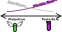
\includegraphics{images/mutpar_continuum.png}

}

\caption{\label{fig-parmut}Parasitism-mutualism continuum of
host-associated microbes. Note that this is a cartoon, and that nature
is in almost all cases more complicated than this.}

\end{figure}%

To phrase the above story a little differently: the microbes in our gut
or in the soil of our favourite crops, are constantly evolving on a
parasitism-mutualism continuum (see Figure~\ref{fig-parmut}). In this
mini project, you will investigate the dynamics of microbiomes evolving
on such a continuum. We will particularly focus on how the properties of
the \emph{host} (plant, animals, etc.) shape the likelihood of disease
outbreaks. To that end, here are a few key questions to get you started,
but you don't need to focus on each and every one of them at the same
time. Plus, more (better!) questions will likely emerge as you work on
the project. That's science.

\section{Key references}\label{key-references}

\begin{itemize}
\tightlist
\item
  Van Vliet and Doebeli (2019): a model of self-sacrificing microbes in
  hosts with different transmission modes.
\item
  Koskella and Bergelson (2020): an opinion piece on host-microbe
  (co)evolution and levels of selection
\end{itemize}

\section{Guiding questions:}\label{guiding-questions}

\begin{itemize}
\tightlist
\item
  Do motile hosts (e.g.~animals) experience different disease pressures
  than non-motile hosts (e.g.~plants)?
\item
  Are mutualistic microbes easier to maintain in short- or long-lived
  hosts?
\item
  Does non-local reproduction (e.g.~seed/spore dispersal) change these
  patterns?
\item
  How does an adaptive immune system (animals) affect the evolution of
  microbiomes, compared to plants, who don't have an adaptive immune
  system?
\end{itemize}

\section{Getting started}\label{getting-started}

Maintaining self-sacrificial microbiomes isn't easy, as shown by the
work of Van Vliet and Doebeli (2019). They show that the evolution of
self-sacrificing microbes (which they call ``helpers'') is highly
sensitive to the host's longevity and transmission of microbes in
between hosts (horizontal transmission). To understand why, start by
reading their paper. If you have read it, unfold the text below to see
my summary of their methods.

\begin{tcolorbox}[enhanced jigsaw, left=2mm, opacitybacktitle=0.6, toptitle=1mm, colbacktitle=quarto-callout-note-color!10!white, toprule=.15mm, coltitle=black, colframe=quarto-callout-note-color-frame, opacityback=0, title=\textcolor{quarto-callout-note-color}{\faInfo}\hspace{0.5em}{My summary of the model by van Vliet et al.}, breakable, bottomtitle=1mm, rightrule=.15mm, titlerule=0mm, arc=.35mm, leftrule=.75mm, bottomrule=.15mm, colback=white]

This model studies the maintanance of self-sacrificial ``helper''
microbes. Here, I will refer to helpers as ``allies'' (A), as to clearly
differentiate it from ``hosts'' (H). Microbes that are not allies are
referred to as neutral (N).

Allies provide a benefit to their host, while neutral microbes do not.
The microbes are modelled with simple ordinary differential equations
(ODEs):

\[
\begin{aligned}
\color{#555}{
\frac{dN}{dt} =
\underbrace{rN}_{\textrm{Growth N}} -
\underbrace{\delta N(A+N)}_{\textrm{Density-dependent death}}
}\\
\color{green}{
  \frac{dA}{dt} =
  \underbrace{rA(1-\gamma)}_{\textrm{Growth A}} -
  \underbrace{\delta A(A+N)}_{\textrm{Density-dependent death}}
}\\
\end{aligned}
\tag{1}
\] As you can see, allies grow slower than neutral microbes and are
therefore at a competitive disadvantage, and will eventually be
outcompeted. To counter-act the loss of allies, van Vliet's model
considers selection at the level of the host. To achieve this, the birth
rate of hosts (\(B_i\)) depends on the frequency of allies A in the
microbiome:

\[
B_i = \frac{r}{G_H}(1+s_b\cdot \frac{A}{A+N})
\]

Here, \(G_H\) is a parameter that scales the host generation time w.r.t.
the growth rate of microbes (\(r\)), with \(G_H \gg r\) ensuring hosts
are long-lived compared to microbes. The term \(s_b\) is the maximum
benefit that hosts get from carrying the ally strain.

The death rate of hosts (\(D_i\)) increases linearly with the density of
hosts at any given time (\(H(t)\)), and is given by:

\[
D_i = \frac{r}{G_H} \frac{H(t)}{K_H}
\]

Where \(H(t)\) gives the number of hosts at a given time, and \(K_H\)
denotes the basal carrying capacity in the absence of allies. Note that
the true carrying capacity can be higher, as helpers increase the birth
rate of hosts.

Whenever a host reproduces, the microbiome is transmitted vertically to
their offspring. The frequency of allies in the offspring is sampled
from a normal distribution with mean \(f_A\):

\[
f_{offspring}  = \mathcal{N} (f_{A},\sigma^2),
\\\text{with } f_A = \frac{A}{A+N}
\]

To avoid negative ally frequencies, this number is truncated such that
\(0<A_{offspring}<1\). The total density in the newborn is set by
another parameter \(n_0\). The model by van Vliet also considers
``horizontal'' transmission of microbiomes, where \(f_A\) is not the
ally frequency in the parent, but the frequency of allies in the
microbiome of a \textbf{random} individual.

So far so good with all the math. Now the simulation\ldots{}

\subsection{The simulation loop}\label{the-simulation-loop}

\begin{enumerate}
\def\labelenumi{\arabic{enumi}.}
\item
  The birth and death rates of all hosts is calculated
\item
  Calculate the probability of a host-level event (birth/death)
  occurring
\item
  If an event occurs, draw a random event proportional to its
  probability.
\item
  Execute the event sampled in step 3
\item
  Update all the microbiome ODEs.
\end{enumerate}

\end{tcolorbox}

To start the project, we will first replicate van Vliet's results in
Python. As a guideline, use my model summary above. I am ready to help
where needed, but at this point in the course your experience should go
a long way! If the simulation works, see if you can reproduce the
following two figures:

\begin{figure}

\begin{minipage}{0.50\linewidth}

\centering{

\includegraphics{images/vliet1.png}

}

\subcaption{\label{fig-vliet1}Allies are maintained within a population
of hosts (black line shows the average), despite each individual host
(green thinner lines) constantly decreasing in ally types. This can be
explained by selection at the level of the host.}

\end{minipage}%
%
\begin{minipage}{0.50\linewidth}

\centering{

\includegraphics{images/vliet2.png}

}

\subcaption{\label{fig-vliet2}Allies are \emph{not} maintained within a
population of hosts (black line shows the average) when transmission of
microbiomes is horizontal (in between random individuals).}

\end{minipage}%

\caption{\label{fig-vliet}Helper maintenance in hosts with different
transmission modes}

\end{figure}%

\section{Extending the model}\label{extending-the-model}

Now that you have a working base-line model, let's extend it to address
the questions we phrased earlier: how does mobility of the host affect
the evolution of microbiomes, and what about non-locally reproducing
fungi? How do these host-level traits affect the likelyhood of
``disease'' outbreaks? Note that so far, we have only discussed
``helpers'' and ``neutral'' microbes, but the same principles apply to
pathogens but perhaps a little more extreme. For example, the microbes
may evolve such high levels of nastiness, that hosts do not only
replicate slower, but die. Think about ways to extend the model that
allows you to tune these distinctions.

\bookmarksetup{startatroot}

\chapter*{References}\label{references-1}
\addcontentsline{toc}{chapter}{References}

\markboth{References}{References}

\phantomsection\label{refs}
\begin{CSLReferences}{1}{0}
\bibitem[\citeproctext]{ref-crombach2008evolution}
Crombach, Anton, and Paulien Hogeweg. 2008. {``Evolution of Evolvability
in Gene Regulatory Networks.''} \emph{PLoS Computational Biology} 4 (7):
e1000112.

\bibitem[\citeproctext]{ref-driever1988bicoid}
Driever, Wolfgang, and Christiane Nüsslein-Volhard. 1988. {``The Bicoid
Protein Determines Position in the Drosophila Embryo in a
Concentration-Dependent Manner.''} \emph{Cell} 54 (1): 95--104.

\bibitem[\citeproctext]{ref-knuth84}
Knuth, Donald E. 1984. {``Literate Programming.''} \emph{Comput. J.} 27
(2): 97--111. \url{https://doi.org/10.1093/comjnl/27.2.97}.

\bibitem[\citeproctext]{ref-koskella2020study}
Koskella, Britt, and Joy Bergelson. 2020. {``The Study of
Host--Microbiome (Co) Evolution Across Levels of Selection.''}
\emph{Philosophical Transactions of the Royal Society B} 375 (1808):
20190604.

\bibitem[\citeproctext]{ref-van2019role}
Van Vliet, Simon, and Michael Doebeli. 2019. {``The Role of Multilevel
Selection in Host Microbiome Evolution.''} \emph{Proceedings of the
National Academy of Sciences} 116 (41): 20591--97.

\bibitem[\citeproctext]{ref-wolpert1969positional}
Wolpert, Lewis. 1969. {``Positional Information and the Spatial Pattern
of Cellular Differentiation.''} \emph{Journal of Theoretical Biology} 25
(1): 1--47.

\end{CSLReferences}

\cleardoublepage
\phantomsection
\addcontentsline{toc}{part}{Appendices}
\appendix

\chapter{Quarto examples}\label{quarto-examples}

\section{Equations}\label{equations-1}

Here's an equation:

\begin{equation}\phantomsection\label{eq-log}{ 
\frac{\mathrm{d}N}{\mathrm{d}t} = rN(1 - \frac{N}{K}) 
}\end{equation}

And Equation~\ref{eq-log} is a reference to the equation above.

\section{References}\label{references-2}

See Knuth (1984) for additional discussion of literate programming.

\section{Syntax highlighting}\label{syntax-highlighting-1}

Here's some python code:

\begin{Shaded}
\begin{Highlighting}[]
\ImportTok{import}\NormalTok{ numpy }\ImportTok{as}\NormalTok{ np}
\NormalTok{np.random.seed(}\DecValTok{42}\NormalTok{)}
\NormalTok{a }\OperatorTok{=} \DecValTok{1} \OperatorTok{+} \DecValTok{2}
\NormalTok{b }\OperatorTok{=}\NormalTok{ a }\OperatorTok{+} \DecValTok{3}
\BuiltInTok{print}\NormalTok{(}\StringTok{"Hello"}\NormalTok{)}
\end{Highlighting}
\end{Shaded}

\section{Visualising data (R)}\label{visualising-data-r-1}

Here's an interactive plot generated with R:

\includegraphics{answers_files/figure-pdf/unnamed-chunk-1-1.pdf}

\section{A youtube clip:}\label{a-youtube-clip-1}

\url{https://www.youtube.com/embed/wo9vZccmqwc}

\section{An `iframe' to a different page (e.g.~my
simulations)}\label{an-iframe-to-a-different-page-e.g.-my-simulations-1}

\subsection{Mermaid}\label{mermaid-1}

Diagrams (Mermaid syntax):

\begin{figure}

\centering{

\includegraphics[width=7.47in,height=2.27in]{answers_files/figure-latex/mermaid-figure-1.png}

}

\caption{\label{fig-variables}Types of models}

\end{figure}%

Which can be referred to Figure~\ref{fig-variables}.

\subsection{Callouts}\label{callouts-1}

Call-outs can organise information and highlight important points.

\begin{tcolorbox}[enhanced jigsaw, left=2mm, opacitybacktitle=0.6, toptitle=1mm, colbacktitle=quarto-callout-note-color!10!white, toprule=.15mm, coltitle=black, colframe=quarto-callout-note-color-frame, opacityback=0, title=\textcolor{quarto-callout-note-color}{\faInfo}\hspace{0.5em}{Note}, breakable, bottomtitle=1mm, rightrule=.15mm, titlerule=0mm, arc=.35mm, leftrule=.75mm, bottomrule=.15mm, colback=white]

Note that there are five types of callouts, including: \texttt{note},
\texttt{warning}, \texttt{important}, \texttt{tip}, and
\texttt{caution}.

\end{tcolorbox}

\begin{tcolorbox}[enhanced jigsaw, left=2mm, opacitybacktitle=0.6, toptitle=1mm, colbacktitle=quarto-callout-tip-color!10!white, toprule=.15mm, coltitle=black, colframe=quarto-callout-tip-color-frame, opacityback=0, title=\textcolor{quarto-callout-tip-color}{\faLightbulb}\hspace{0.5em}{Tip with Title}, breakable, bottomtitle=1mm, rightrule=.15mm, titlerule=0mm, arc=.35mm, leftrule=.75mm, bottomrule=.15mm, colback=white]

This is an example of a callout with a title.

\end{tcolorbox}

\begin{tcolorbox}[enhanced jigsaw, left=2mm, opacitybacktitle=0.6, toptitle=1mm, colbacktitle=quarto-callout-caution-color!10!white, toprule=.15mm, coltitle=black, colframe=quarto-callout-caution-color-frame, opacityback=0, title=\textcolor{quarto-callout-caution-color}{\faFire}\hspace{0.5em}{Expand To Learn About Collapse}, breakable, bottomtitle=1mm, rightrule=.15mm, titlerule=0mm, arc=.35mm, leftrule=.75mm, bottomrule=.15mm, colback=white]

This is an example of a `folded' caution callout that can be expanded by
the user. You can use \texttt{collapse="true"} to collapse it by default
or \texttt{collapse="false"} to make a collapsible callout that is
expanded by default.

\end{tcolorbox}

\begin{tcolorbox}[enhanced jigsaw, left=2mm, opacitybacktitle=0.6, toptitle=1mm, colbacktitle=quarto-callout-tip-color!10!white, toprule=.15mm, coltitle=black, colframe=quarto-callout-tip-color-frame, opacityback=0, title=\textcolor{quarto-callout-tip-color}{\faLightbulb}\hspace{0.5em}{Tip \ref*{tip-example}: Cross-Referencing a Tip}, breakable, bottomtitle=1mm, rightrule=.15mm, titlerule=0mm, arc=.35mm, leftrule=.75mm, bottomrule=.15mm, colback=white]

\quartocallouttip{tip-example} 

Add an ID starting with \texttt{\#tip-} to reference a tip.

\end{tcolorbox}

See Tip~\ref{tip-example}\ldots{}

\subsection{How to format questions/problem
sets}\label{how-to-format-questionsproblem-sets-1}

\begin{exercise}[Test
1]\protect\hypertarget{exr-test1}{}\label{exr-test1}

The equation of any straight line, called a linear equation, can be
written as:

\begin{equation}\phantomsection\label{eq-line}{ 
y = mx + b
}\end{equation}

Refer to the equation like this Equation~\ref{eq-line} or like
Customlabel~\ref{eq-line}.

\textbf{a.} Blabla?

\textbf{b.} Of blablabla?

\end{exercise}

\subsection{Sharing data tables:}\label{sharing-data-tables-1}

\includegraphics{answers_files/figure-pdf/tab-anscombe-1.pdf}




\end{document}
